\documentclass[twoside]{book}

% Packages required by doxygen
\usepackage{fixltx2e}
\usepackage{calc}
\usepackage{doxygen}
\usepackage[export]{adjustbox} % also loads graphicx
\usepackage{graphicx}
\usepackage[utf8]{inputenc}
\usepackage{makeidx}
\usepackage{multicol}
\usepackage{multirow}
\PassOptionsToPackage{warn}{textcomp}
\usepackage{textcomp}
\usepackage[nointegrals]{wasysym}
\usepackage[table]{xcolor}

% Font selection
\usepackage[T1]{fontenc}
\usepackage[scaled=.90]{helvet}
\usepackage{courier}
\usepackage{amssymb}
\usepackage{sectsty}
\renewcommand{\familydefault}{\sfdefault}
\allsectionsfont{%
  \fontseries{bc}\selectfont%
  \color{darkgray}%
}
\renewcommand{\DoxyLabelFont}{%
  \fontseries{bc}\selectfont%
  \color{darkgray}%
}
\newcommand{\+}{\discretionary{\mbox{\scriptsize$\hookleftarrow$}}{}{}}

% Page & text layout
\usepackage{geometry}
\geometry{%
  a4paper,%
  top=2.5cm,%
  bottom=2.5cm,%
  left=2.5cm,%
  right=2.5cm%
}
\tolerance=750
\hfuzz=15pt
\hbadness=750
\setlength{\emergencystretch}{15pt}
\setlength{\parindent}{0cm}
\setlength{\parskip}{3ex plus 2ex minus 2ex}
\makeatletter
\renewcommand{\paragraph}{%
  \@startsection{paragraph}{4}{0ex}{-1.0ex}{1.0ex}{%
    \normalfont\normalsize\bfseries\SS@parafont%
  }%
}
\renewcommand{\subparagraph}{%
  \@startsection{subparagraph}{5}{0ex}{-1.0ex}{1.0ex}{%
    \normalfont\normalsize\bfseries\SS@subparafont%
  }%
}
\makeatother

% Headers & footers
\usepackage{fancyhdr}
\pagestyle{fancyplain}
\fancyhead[LE]{\fancyplain{}{\bfseries\thepage}}
\fancyhead[CE]{\fancyplain{}{}}
\fancyhead[RE]{\fancyplain{}{\bfseries\leftmark}}
\fancyhead[LO]{\fancyplain{}{\bfseries\rightmark}}
\fancyhead[CO]{\fancyplain{}{}}
\fancyhead[RO]{\fancyplain{}{\bfseries\thepage}}
\fancyfoot[LE]{\fancyplain{}{}}
\fancyfoot[CE]{\fancyplain{}{}}
\fancyfoot[RE]{\fancyplain{}{\bfseries\scriptsize Generated by Doxygen }}
\fancyfoot[LO]{\fancyplain{}{\bfseries\scriptsize Generated by Doxygen }}
\fancyfoot[CO]{\fancyplain{}{}}
\fancyfoot[RO]{\fancyplain{}{}}
\renewcommand{\footrulewidth}{0.4pt}
\renewcommand{\chaptermark}[1]{%
  \markboth{#1}{}%
}
\renewcommand{\sectionmark}[1]{%
  \markright{\thesection\ #1}%
}

% Indices & bibliography
\usepackage{natbib}
\usepackage[titles]{tocloft}
\setcounter{tocdepth}{3}
\setcounter{secnumdepth}{5}
\makeindex

% Hyperlinks (required, but should be loaded last)
\usepackage{ifpdf}
\ifpdf
  \usepackage[pdftex,pagebackref=true]{hyperref}
\else
  \usepackage[ps2pdf,pagebackref=true]{hyperref}
\fi
\hypersetup{%
  colorlinks=true,%
  linkcolor=blue,%
  citecolor=blue,%
  unicode%
}

% Custom commands
\newcommand{\clearemptydoublepage}{%
  \newpage{\pagestyle{empty}\cleardoublepage}%
}

\usepackage{caption}
\captionsetup{labelsep=space,justification=centering,font={bf},singlelinecheck=off,skip=4pt,position=top}

%===== C O N T E N T S =====

\begin{document}

% Titlepage & ToC
\hypersetup{pageanchor=false,
             bookmarksnumbered=true,
             pdfencoding=unicode
            }
\pagenumbering{alph}
\begin{titlepage}
\vspace*{7cm}
\begin{center}%
{\Large coolcats }\\
\vspace*{1cm}
{\large Generated by Doxygen 1.8.13}\\
\end{center}
\end{titlepage}
\clearemptydoublepage
\pagenumbering{roman}
\tableofcontents
\clearemptydoublepage
\pagenumbering{arabic}
\hypersetup{pageanchor=true}

%--- Begin generated contents ---
\chapter{R\+E\+A\+D\+ME}
\label{md__r_e_a_d_m_e}
\Hypertarget{md__r_e_a_d_m_e}
\#include $<$dad$>$

This is the Readme for the ultra secret project known as \#include $<$dad$>$.

Or more specifically as the \char`\"{}\+Meme Maker 2000\char`\"{}. 
\chapter{Hierarchical Index}
\section{Class Hierarchy}
This inheritance list is sorted roughly, but not completely, alphabetically\+:\begin{DoxyCompactList}
\item Q\+Dialog\begin{DoxyCompactList}
\item \contentsline{section}{Contact}{\pageref{class_contact}}{}
\item \contentsline{section}{Help}{\pageref{class_help}}{}
\item \contentsline{section}{Maintenance\+Notes}{\pageref{class_maintenance_notes}}{}
\item \contentsline{section}{newnew}{\pageref{classnewnew}}{}
\item \contentsline{section}{Testimonials}{\pageref{class_testimonials}}{}
\end{DoxyCompactList}
\item Q\+Main\+Window\begin{DoxyCompactList}
\item \contentsline{section}{Login\+Screen}{\pageref{class_login_screen}}{}
\item \contentsline{section}{Main\+Interface}{\pageref{class_main_interface}}{}
\end{DoxyCompactList}
\item Q\+Widget\begin{DoxyCompactList}
\item \contentsline{section}{Canvas}{\pageref{class_canvas}}{}
\end{DoxyCompactList}
\item \contentsline{section}{Shape}{\pageref{class_shape}}{}
\begin{DoxyCompactList}
\item \contentsline{section}{Ellipse}{\pageref{class_ellipse}}{}
\begin{DoxyCompactList}
\item \contentsline{section}{Circle}{\pageref{class_circle}}{}
\end{DoxyCompactList}
\item \contentsline{section}{Line}{\pageref{class_line}}{}
\begin{DoxyCompactList}
\item \contentsline{section}{Poly\+Line}{\pageref{class_poly_line}}{}
\begin{DoxyCompactList}
\item \contentsline{section}{Polygon}{\pageref{class_polygon}}{}
\end{DoxyCompactList}
\end{DoxyCompactList}
\item \contentsline{section}{Rectangle}{\pageref{class_rectangle}}{}
\begin{DoxyCompactList}
\item \contentsline{section}{Square}{\pageref{class_square}}{}
\end{DoxyCompactList}
\end{DoxyCompactList}
\item \contentsline{section}{single\+User}{\pageref{structsingle_user}}{}
\item \contentsline{section}{Ui\+\_\+\+Contact}{\pageref{class_ui___contact}}{}
\begin{DoxyCompactList}
\item \contentsline{section}{Ui\+:\+:Contact}{\pageref{class_ui_1_1_contact}}{}
\end{DoxyCompactList}
\item \contentsline{section}{Ui\+\_\+\+Dialog}{\pageref{class_ui___dialog}}{}
\begin{DoxyCompactList}
\item \contentsline{section}{Ui\+:\+:Dialog}{\pageref{class_ui_1_1_dialog}}{}
\end{DoxyCompactList}
\item \contentsline{section}{Ui\+\_\+\+Help}{\pageref{class_ui___help}}{}
\begin{DoxyCompactList}
\item \contentsline{section}{Ui\+:\+:Help}{\pageref{class_ui_1_1_help}}{}
\end{DoxyCompactList}
\item \contentsline{section}{Ui\+\_\+\+Login\+Screen}{\pageref{class_ui___login_screen}}{}
\begin{DoxyCompactList}
\item \contentsline{section}{Ui\+:\+:Login\+Screen}{\pageref{class_ui_1_1_login_screen}}{}
\end{DoxyCompactList}
\item \contentsline{section}{Ui\+\_\+\+Main\+Interface}{\pageref{class_ui___main_interface}}{}
\begin{DoxyCompactList}
\item \contentsline{section}{Ui\+:\+:Main\+Interface}{\pageref{class_ui_1_1_main_interface}}{}
\end{DoxyCompactList}
\item \contentsline{section}{Ui\+\_\+\+Maintenance\+Notes}{\pageref{class_ui___maintenance_notes}}{}
\begin{DoxyCompactList}
\item \contentsline{section}{Ui\+:\+:Maintenance\+Notes}{\pageref{class_ui_1_1_maintenance_notes}}{}
\end{DoxyCompactList}
\item \contentsline{section}{Ui\+\_\+newnew}{\pageref{class_ui__newnew}}{}
\begin{DoxyCompactList}
\item \contentsline{section}{Ui\+:\+:newnew}{\pageref{class_ui_1_1newnew}}{}
\end{DoxyCompactList}
\item \contentsline{section}{Ui\+\_\+\+Testimonials}{\pageref{class_ui___testimonials}}{}
\begin{DoxyCompactList}
\item \contentsline{section}{Ui\+:\+:Testimonials}{\pageref{class_ui_1_1_testimonials}}{}
\end{DoxyCompactList}
\item \contentsline{section}{User\+List}{\pageref{class_user_list}}{}
\item \contentsline{section}{Vector$<$ Type $>$}{\pageref{class_vector}}{}
\item \contentsline{section}{Vector$<$ Shape $\ast$$>$}{\pageref{class_vector}}{}
\item \contentsline{section}{Vector$<$ single\+User $>$}{\pageref{class_vector}}{}
\end{DoxyCompactList}

\chapter{Class Index}
\section{Class List}
Here are the classes, structs, unions and interfaces with brief descriptions\+:\begin{DoxyCompactList}
\item\contentsline{section}{\hyperlink{class_canvas}{Canvas} \\*The \hyperlink{class_canvas}{Canvas} class This class is a modified Q\+Widget that will define an area on which 2d objects will be rendered. It gets and receives mouse inputs for moving object, and mouse inputs for getting points for the geometric shapes\+: \hyperlink{class_line}{Line}, Polyline, Poly\+Gon. Based on which shape is selected it allows the user to change it using dynamic casting of the \hyperlink{class_shape}{Shape} Pointer and shape specific mutators }{\pageref{class_canvas}}{}
\item\contentsline{section}{\hyperlink{class_circle}{Circle} \\*The \hyperlink{class_circle}{Circle} class }{\pageref{class_circle}}{}
\item\contentsline{section}{\hyperlink{class_ui_1_1_contact}{Ui\+::\+Contact} }{\pageref{class_ui_1_1_contact}}{}
\item\contentsline{section}{\hyperlink{class_contact}{Contact} }{\pageref{class_contact}}{}
\item\contentsline{section}{\hyperlink{class_ui_1_1_dialog}{Ui\+::\+Dialog} }{\pageref{class_ui_1_1_dialog}}{}
\item\contentsline{section}{\hyperlink{class_ellipse}{Ellipse} \\*
\begin{DoxyItemize}
\item parent to circle class, handles move functions as well as area and perimeter coming from the virtual base class 
\end{DoxyItemize}}{\pageref{class_ellipse}}{}
\item\contentsline{section}{\hyperlink{class_help}{Help} }{\pageref{class_help}}{}
\item\contentsline{section}{\hyperlink{class_ui_1_1_help}{Ui\+::\+Help} }{\pageref{class_ui_1_1_help}}{}
\item\contentsline{section}{\hyperlink{class_line}{Line} \\*
\begin{DoxyItemize}
\item derived from the abstarct shape class\+: can manipulate all of the pen and brush styles and colors 
\end{DoxyItemize}}{\pageref{class_line}}{}
\item\contentsline{section}{\hyperlink{class_ui_1_1_login_screen}{Ui\+::\+Login\+Screen} }{\pageref{class_ui_1_1_login_screen}}{}
\item\contentsline{section}{\hyperlink{class_login_screen}{Login\+Screen} \\*
\begin{DoxyItemize}
\item obsolete\+:replaced by newnew.\+ui 
\end{DoxyItemize}}{\pageref{class_login_screen}}{}
\item\contentsline{section}{\hyperlink{class_main_interface}{Main\+Interface} \\*Hold all of the shape classes, handles the changing of shapes via public methods; changing all of the pen and brush styles as well as method that returns the area/perimeter of said shapes }{\pageref{class_main_interface}}{}
\item\contentsline{section}{\hyperlink{class_ui_1_1_main_interface}{Ui\+::\+Main\+Interface} }{\pageref{class_ui_1_1_main_interface}}{}
\item\contentsline{section}{\hyperlink{class_maintenance_notes}{Maintenance\+Notes} }{\pageref{class_maintenance_notes}}{}
\item\contentsline{section}{\hyperlink{class_ui_1_1_maintenance_notes}{Ui\+::\+Maintenance\+Notes} }{\pageref{class_ui_1_1_maintenance_notes}}{}
\item\contentsline{section}{\hyperlink{classnewnew}{newnew} \\*
\begin{DoxyItemize}
\item this is the new login window it handles creating new users as well as checking already exsisting users via the user\+Object object containg a vector of all the exsisting users 
\end{DoxyItemize}}{\pageref{classnewnew}}{}
\item\contentsline{section}{\hyperlink{class_ui_1_1newnew}{Ui\+::newnew} }{\pageref{class_ui_1_1newnew}}{}
\item\contentsline{section}{\hyperlink{class_polygon}{Polygon} \\*
\begin{DoxyItemize}
\item derives form the Polyline class set to make polygon shapes 
\end{DoxyItemize}}{\pageref{class_polygon}}{}
\item\contentsline{section}{\hyperlink{class_poly_line}{Poly\+Line} \\*
\begin{DoxyItemize}
\item derives from line 
\end{DoxyItemize}}{\pageref{class_poly_line}}{}
\item\contentsline{section}{\hyperlink{class_rectangle}{Rectangle} \\*
\begin{DoxyItemize}
\item derives from abstract base class\+: shape 
\end{DoxyItemize}}{\pageref{class_rectangle}}{}
\item\contentsline{section}{\hyperlink{class_shape}{Shape} \\*
\begin{DoxyItemize}
\item base abstract class-\/parent to all other shape classes-\/holds all of the private data types that change or access pen/brush attributes; is also what is held in the shape vector class 
\end{DoxyItemize}}{\pageref{class_shape}}{}
\item\contentsline{section}{\hyperlink{structsingle_user}{single\+User} \\*The \hyperlink{structsingle_user}{single\+User} struct -\/ user information held in a struct }{\pageref{structsingle_user}}{}
\item\contentsline{section}{\hyperlink{class_square}{Square} }{\pageref{class_square}}{}
\item\contentsline{section}{\hyperlink{class_ui_1_1_testimonials}{Ui\+::\+Testimonials} }{\pageref{class_ui_1_1_testimonials}}{}
\item\contentsline{section}{\hyperlink{class_testimonials}{Testimonials} }{\pageref{class_testimonials}}{}
\item\contentsline{section}{\hyperlink{class_ui___contact}{Ui\+\_\+\+Contact} }{\pageref{class_ui___contact}}{}
\item\contentsline{section}{\hyperlink{class_ui___dialog}{Ui\+\_\+\+Dialog} }{\pageref{class_ui___dialog}}{}
\item\contentsline{section}{\hyperlink{class_ui___help}{Ui\+\_\+\+Help} }{\pageref{class_ui___help}}{}
\item\contentsline{section}{\hyperlink{class_ui___login_screen}{Ui\+\_\+\+Login\+Screen} }{\pageref{class_ui___login_screen}}{}
\item\contentsline{section}{\hyperlink{class_ui___main_interface}{Ui\+\_\+\+Main\+Interface} }{\pageref{class_ui___main_interface}}{}
\item\contentsline{section}{\hyperlink{class_ui___maintenance_notes}{Ui\+\_\+\+Maintenance\+Notes} }{\pageref{class_ui___maintenance_notes}}{}
\item\contentsline{section}{\hyperlink{class_ui__newnew}{Ui\+\_\+newnew} }{\pageref{class_ui__newnew}}{}
\item\contentsline{section}{\hyperlink{class_ui___testimonials}{Ui\+\_\+\+Testimonials} }{\pageref{class_ui___testimonials}}{}
\item\contentsline{section}{\hyperlink{class_user_list}{User\+List} \\*
\begin{DoxyItemize}
\item holds a vector of all the users that are registered within our program; has public methods to manipulate and access all of the said users inside of the vector 
\end{DoxyItemize}}{\pageref{class_user_list}}{}
\item\contentsline{section}{\hyperlink{class_vector}{Vector$<$ Type $>$} \\*The \hyperlink{class_vector}{Vector} class -\/ the templated vector class that is used mainly as a way to store all of the shape pointers that will be drawn on the canvas this was given to us in class; with little modification to some of the functions works very similar to the S\+TL vector }{\pageref{class_vector}}{}
\end{DoxyCompactList}

\chapter{Class Documentation}
\hypertarget{class_canvas}{}\section{Canvas Class Reference}
\label{class_canvas}\index{Canvas@{Canvas}}


The \hyperlink{class_canvas}{Canvas} class This class is a modified Q\+Widget that will define an area on which 2d objects will be rendered. It gets and receives mouse inputs for moving object, and mouse inputs for getting points for the geometric shapes\+: \hyperlink{class_line}{Line}, Polyline, Poly\+Gon. Based on which shape is selected it allows the user to change it using dynamic casting of the \hyperlink{class_shape}{Shape} Pointer and shape specific mutators.  




{\ttfamily \#include $<$canvas.\+h$>$}

Inheritance diagram for Canvas\+:\begin{figure}[H]
\begin{center}
\leavevmode
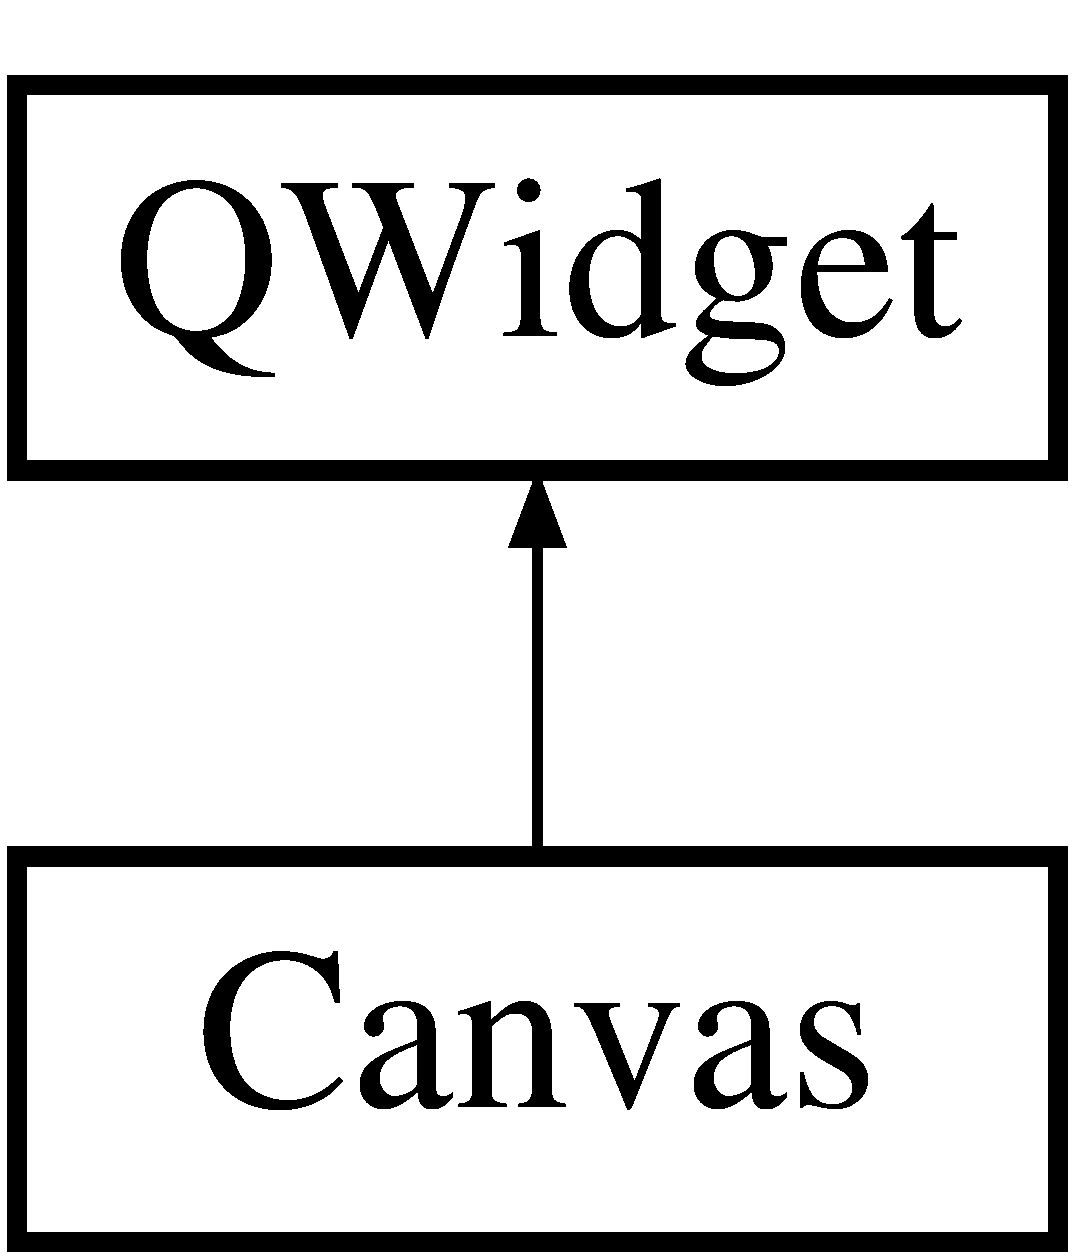
\includegraphics[height=2.000000cm]{class_canvas}
\end{center}
\end{figure}
\subsection*{Public Slots}
\begin{DoxyCompactItemize}
\item 
\mbox{\Hypertarget{class_canvas_a100162adb347f04ad3ec5ce0c2e118f7}\label{class_canvas_a100162adb347f04ad3ec5ce0c2e118f7}} 
void {\bfseries mouse\+Point\+Input} ()
\end{DoxyCompactItemize}
\subsection*{Signals}
\begin{DoxyCompactItemize}
\item 
\mbox{\Hypertarget{class_canvas_ab17abdfec6f1ca1d682420f0a124e8f4}\label{class_canvas_ab17abdfec6f1ca1d682420f0a124e8f4}} 
void {\bfseries is\+Clicked} ()
\end{DoxyCompactItemize}
\subsection*{Public Member Functions}
\begin{DoxyCompactItemize}
\item 
\mbox{\Hypertarget{class_canvas_a5525075d65b32480dd518d382946e0ea}\label{class_canvas_a5525075d65b32480dd518d382946e0ea}} 
{\bfseries Canvas} (Q\+Widget $\ast$parent=0)
\item 
\mbox{\Hypertarget{class_canvas_a2e467a527500d7936c510db72e154ce6}\label{class_canvas_a2e467a527500d7936c510db72e154ce6}} 
void {\bfseries add\+Shape} (\hyperlink{class_shape}{Shape} $\ast$add)
\item 
\mbox{\Hypertarget{class_canvas_ac4bf60e8e094e90a16a4b525e89889ec}\label{class_canvas_ac4bf60e8e094e90a16a4b525e89889ec}} 
\hyperlink{class_shape}{Shape} $\ast$ {\bfseries get\+Current\+Shape} ()
\item 
\mbox{\Hypertarget{class_canvas_abfa07c6ffae9507dd2bff77ef26db804}\label{class_canvas_abfa07c6ffae9507dd2bff77ef26db804}} 
int {\bfseries get\+Shape\+Num} () const
\item 
\mbox{\Hypertarget{class_canvas_ab973843b8722be986bb17ee02ca47488}\label{class_canvas_ab973843b8722be986bb17ee02ca47488}} 
void {\bfseries set\+Current\+Shape} (\hyperlink{class_shape}{Shape} $\ast$e)
\item 
\mbox{\Hypertarget{class_canvas_ac4559a6535f497f17415032632aa9f6a}\label{class_canvas_ac4559a6535f497f17415032632aa9f6a}} 
void {\bfseries clear} ()
\item 
\mbox{\Hypertarget{class_canvas_a47b2f0b05d0aaeb93029e28cb2228746}\label{class_canvas_a47b2f0b05d0aaeb93029e28cb2228746}} 
void {\bfseries render} ()
\item 
\mbox{\Hypertarget{class_canvas_a96fdffb7f3f92b4522e3c320e151ac72}\label{class_canvas_a96fdffb7f3f92b4522e3c320e151ac72}} 
\hyperlink{class_shape}{Shape} \& {\bfseries operator\mbox{[}$\,$\mbox{]}} (int x)
\end{DoxyCompactItemize}
\subsection*{Protected Member Functions}
\begin{DoxyCompactItemize}
\item 
\mbox{\Hypertarget{class_canvas_abc2200972cf33fd8991d4759955eb0d8}\label{class_canvas_abc2200972cf33fd8991d4759955eb0d8}} 
void {\bfseries mouse\+Press\+Event} (Q\+Mouse\+Event $\ast$event)
\item 
\mbox{\Hypertarget{class_canvas_a9fb4b83a1067ddc2aa04676f51dc5a47}\label{class_canvas_a9fb4b83a1067ddc2aa04676f51dc5a47}} 
void {\bfseries mouse\+Move\+Event} (Q\+Mouse\+Event $\ast$event)
\item 
\mbox{\Hypertarget{class_canvas_a0e5ff2b8662659da1687eb31ad41d119}\label{class_canvas_a0e5ff2b8662659da1687eb31ad41d119}} 
void {\bfseries paint\+Event} (Q\+Paint\+Event $\ast$)
\item 
\mbox{\Hypertarget{class_canvas_a3bcc6c012c67e727125cf2d138e944b8}\label{class_canvas_a3bcc6c012c67e727125cf2d138e944b8}} 
void {\bfseries key\+Press\+Event} (Q\+Key\+Event $\ast$key)
\end{DoxyCompactItemize}


\subsection{Detailed Description}
The \hyperlink{class_canvas}{Canvas} class This class is a modified Q\+Widget that will define an area on which 2d objects will be rendered. It gets and receives mouse inputs for moving object, and mouse inputs for getting points for the geometric shapes\+: \hyperlink{class_line}{Line}, Polyline, Poly\+Gon. Based on which shape is selected it allows the user to change it using dynamic casting of the \hyperlink{class_shape}{Shape} Pointer and shape specific mutators. 

The documentation for this class was generated from the following files\+:\begin{DoxyCompactItemize}
\item 
canvas.\+h\item 
canvas.\+cpp\end{DoxyCompactItemize}

\hypertarget{class_circle}{}\section{Circle Class Reference}
\label{class_circle}\index{Circle@{Circle}}


The \hyperlink{class_circle}{Circle} class.  




{\ttfamily \#include $<$Circle.\+h$>$}

Inheritance diagram for Circle\+:\begin{figure}[H]
\begin{center}
\leavevmode
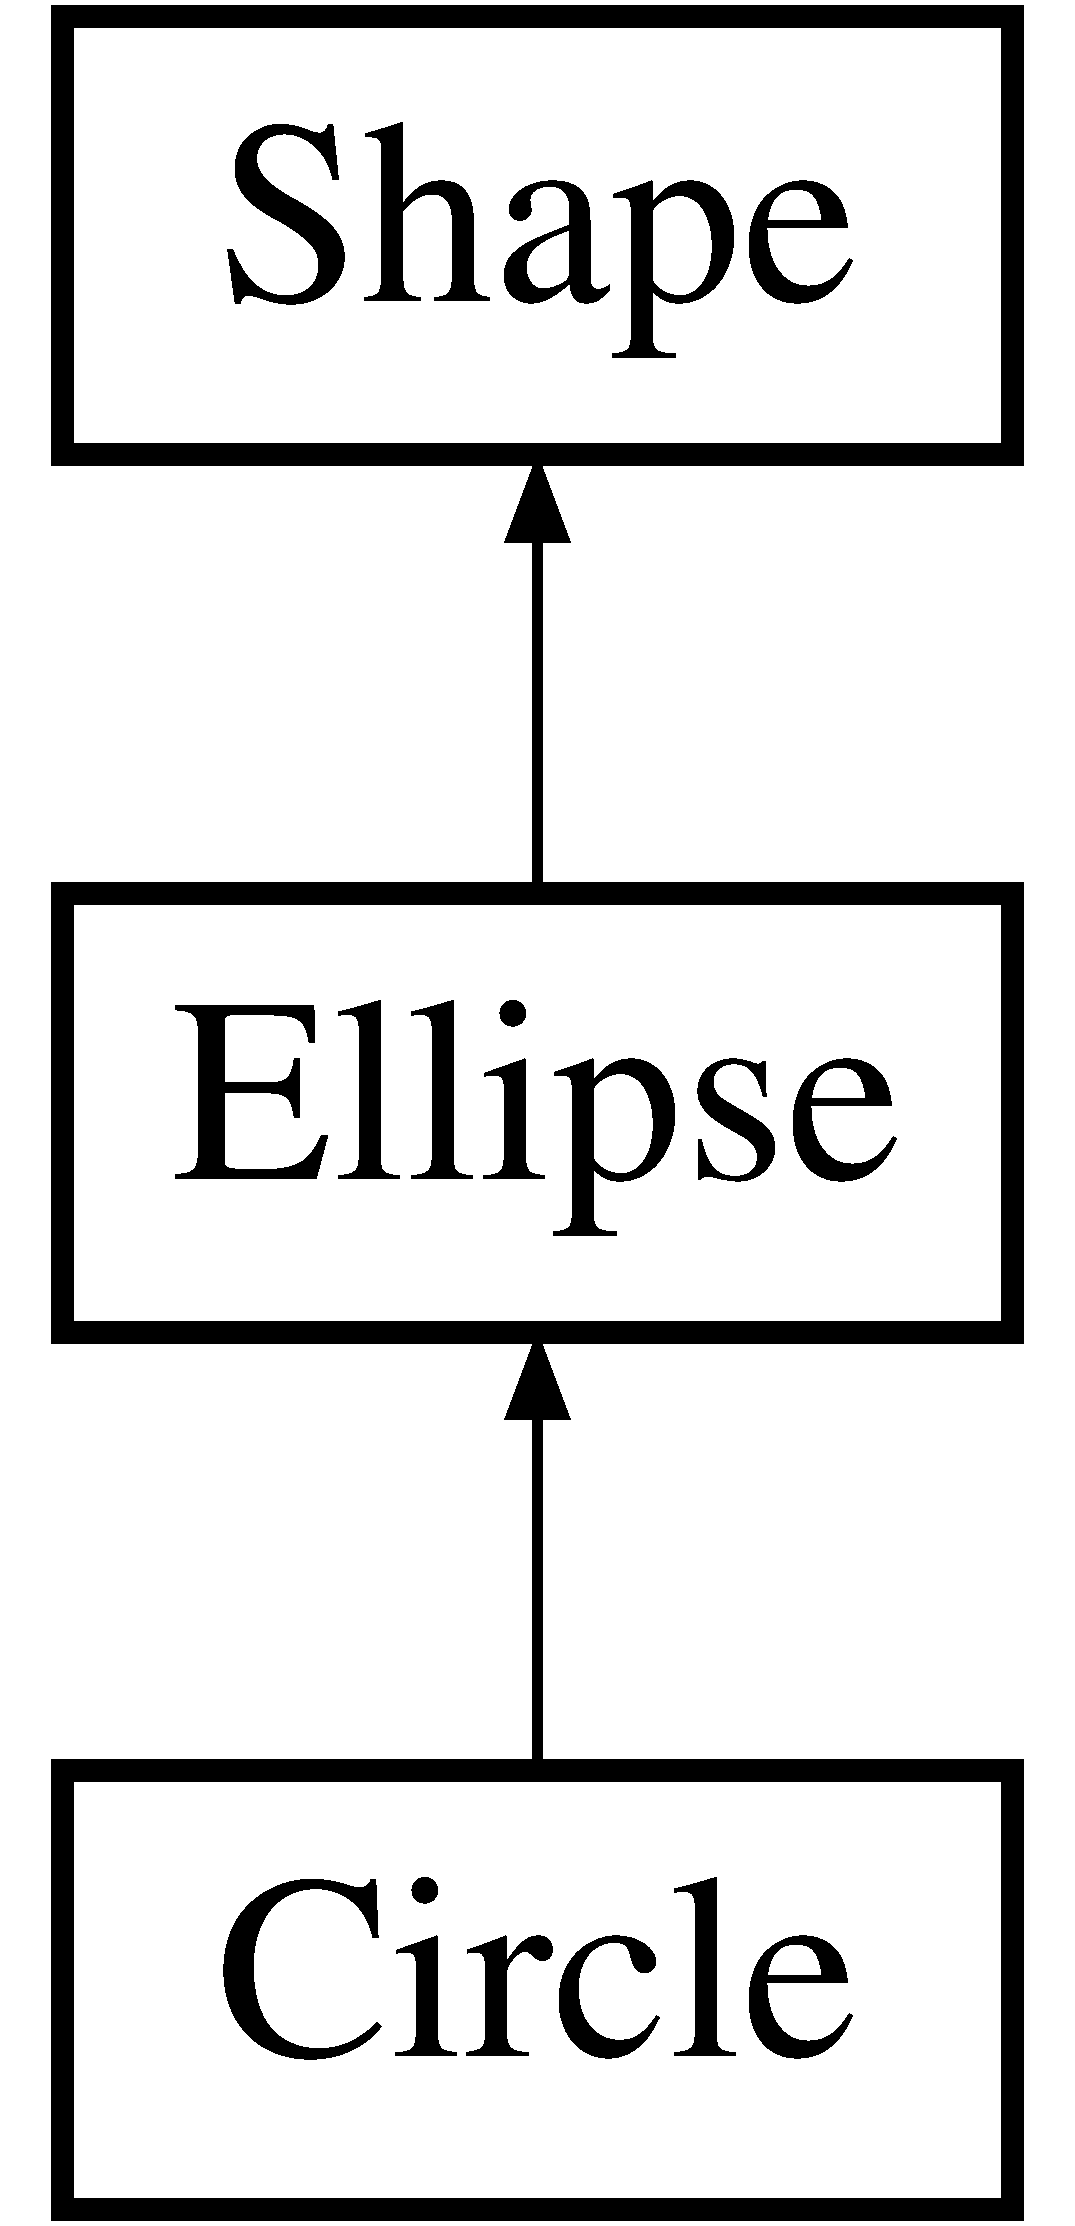
\includegraphics[height=3.000000cm]{class_circle}
\end{center}
\end{figure}
\subsection*{Public Member Functions}
\begin{DoxyCompactItemize}
\item 
\mbox{\Hypertarget{class_circle_ab672be11e6bca406b9c4f3feb4b4aad3}\label{class_circle_ab672be11e6bca406b9c4f3feb4b4aad3}} 
{\bfseries Circle} (int x\+In, int y\+In, double radius\+In)
\item 
\hyperlink{class_circle_a4b41e38613114920686bbfea15ded361}{Circle} (Q\+String id\+In, Qt\+::\+Brush\+Style brush\+Style\+In, Qt\+::\+Global\+Color brush\+Color\+In, double pen\+Width\+In, Qt\+::\+Global\+Color pen\+Color\+In, Qt\+::\+Pen\+Cap\+Style pen\+Cap\+In, Qt\+::\+Pen\+Join\+Style pen\+Join\+In, Qt\+::\+Pen\+Style pen\+Style\+In, double xR)
\begin{DoxyCompactList}\small\item\em Circle\+::\+Circle A class that will render a circle based on the params. It will only render to the custom type canvas. \end{DoxyCompactList}\item 
\mbox{\Hypertarget{class_circle_a5df00ac5563cbef6e87faa7f2c2a446b}\label{class_circle_a5df00ac5563cbef6e87faa7f2c2a446b}} 
{\bfseries Circle} (\hyperlink{class_circle}{Circle} \&copy)
\item 
\mbox{\Hypertarget{class_circle_a3e4cff49aa70b470ca6abb2923970d80}\label{class_circle_a3e4cff49aa70b470ca6abb2923970d80}} 
{\bfseries Circle} (\hyperlink{class_circle}{Circle} \&\&copy)
\item 
\mbox{\Hypertarget{class_circle_a99fe1cbabbf3a9ccae51832376c5e8d4}\label{class_circle_a99fe1cbabbf3a9ccae51832376c5e8d4}} 
double {\bfseries get\+Area} ()
\item 
\mbox{\Hypertarget{class_circle_afee5f4743c89e48e462e5f56aa605669}\label{class_circle_afee5f4743c89e48e462e5f56aa605669}} 
double {\bfseries get\+Perimeter} ()
\item 
virtual void \hyperlink{class_circle_a6ed1a2d29c5dc49a2ae3051449576577}{move} (int x\+Des, int y\+Des)
\begin{DoxyCompactList}\small\item\em \hyperlink{class_circle_a6ed1a2d29c5dc49a2ae3051449576577}{Circle\+::move}. \end{DoxyCompactList}\item 
virtual void \hyperlink{class_circle_a5f02de3ad7e992a689b9f9e88643076c}{move} (Q\+Point xy)
\begin{DoxyCompactList}\small\item\em move -\/ handles moving the shape and recieves in mouse input \end{DoxyCompactList}\item 
\mbox{\Hypertarget{class_circle_a1d04f83b447f9e4a03cca186b929e083}\label{class_circle_a1d04f83b447f9e4a03cca186b929e083}} 
virtual void {\bfseries Resize} (double radius\+In)
\item 
virtual void \hyperlink{class_circle_a5bebd94955572edce0ad10208a449772}{Draw} (\hyperlink{class_canvas}{Canvas} $\ast$area)
\begin{DoxyCompactList}\small\item\em Draw -\/ draws the shape\+: virtual. \end{DoxyCompactList}\item 
virtual bool \hyperlink{class_circle_a1661bb4e324cce0196a6aa1195c26c73}{is\+\_\+\+Left\+\_\+\+Clicked} (Q\+Point e)
\begin{DoxyCompactList}\small\item\em \hyperlink{class_circle_a1661bb4e324cce0196a6aa1195c26c73}{Circle\+::is\+\_\+\+Left\+\_\+\+Clicked}. \end{DoxyCompactList}\end{DoxyCompactItemize}
\subsection*{Additional Inherited Members}


\subsection{Detailed Description}
The \hyperlink{class_circle}{Circle} class. 


\begin{DoxyItemize}
\item derived from the ellipse class 
\end{DoxyItemize}

\subsection{Constructor \& Destructor Documentation}
\mbox{\Hypertarget{class_circle_a4b41e38613114920686bbfea15ded361}\label{class_circle_a4b41e38613114920686bbfea15ded361}} 
\index{Circle@{Circle}!Circle@{Circle}}
\index{Circle@{Circle}!Circle@{Circle}}
\subsubsection{\texorpdfstring{Circle()}{Circle()}}
{\footnotesize\ttfamily Circle\+::\+Circle (\begin{DoxyParamCaption}\item[{Q\+String}]{id\+In,  }\item[{Qt\+::\+Brush\+Style}]{brush\+Style\+In,  }\item[{Qt\+::\+Global\+Color}]{brush\+Color\+In,  }\item[{double}]{pen\+Width\+In,  }\item[{Qt\+::\+Global\+Color}]{pen\+Color\+In,  }\item[{Qt\+::\+Pen\+Cap\+Style}]{pen\+Cap\+In,  }\item[{Qt\+::\+Pen\+Join\+Style}]{pen\+Join\+In,  }\item[{Qt\+::\+Pen\+Style}]{pen\+Style\+In,  }\item[{double}]{xR }\end{DoxyParamCaption})}



Circle\+::\+Circle A class that will render a circle based on the params. It will only render to the custom type canvas. 


\begin{DoxyParams}{Parameters}
{\em id\+In} & -\/ specifies the string that represents the object \\
\hline
{\em brush\+Style\+In} & -\/ specifies the style of the brush \\
\hline
{\em brush\+Color\+In} & -\/ specifies the brush\textquotesingle{}s color \\
\hline
{\em pen\+Width\+In} & -\/ specifies the width of the pen \\
\hline
{\em pen\+Color\+In} & -\/ Specifies the Color of the pen \\
\hline
{\em pen\+Cap\+In} & -\/ Specifies how the end of the line will cap. \\
\hline
{\em pen\+Join\+In} & -\/ Specifies how the pen will join. \\
\hline
{\em pen\+Style\+In} & -\/ The style of the pen. \\
\hline
{\em xR} & -\/ The Radius of the circle goemetric object \\
\hline
\end{DoxyParams}


\subsection{Member Function Documentation}
\mbox{\Hypertarget{class_circle_a5bebd94955572edce0ad10208a449772}\label{class_circle_a5bebd94955572edce0ad10208a449772}} 
\index{Circle@{Circle}!Draw@{Draw}}
\index{Draw@{Draw}!Circle@{Circle}}
\subsubsection{\texorpdfstring{Draw()}{Draw()}}
{\footnotesize\ttfamily void Circle\+::\+Draw (\begin{DoxyParamCaption}\item[{\hyperlink{class_canvas}{Canvas} $\ast$}]{paint\+Area }\end{DoxyParamCaption})\hspace{0.3cm}{\ttfamily [virtual]}}



Draw -\/ draws the shape\+: virtual. 


\begin{DoxyParams}{Parameters}
{\em paint\+Area} & \\
\hline
\end{DoxyParams}


Reimplemented from \hyperlink{class_ellipse_aaf9524151dc799501327f72c75e0f010}{Ellipse}.

\mbox{\Hypertarget{class_circle_a1661bb4e324cce0196a6aa1195c26c73}\label{class_circle_a1661bb4e324cce0196a6aa1195c26c73}} 
\index{Circle@{Circle}!is\+\_\+\+Left\+\_\+\+Clicked@{is\+\_\+\+Left\+\_\+\+Clicked}}
\index{is\+\_\+\+Left\+\_\+\+Clicked@{is\+\_\+\+Left\+\_\+\+Clicked}!Circle@{Circle}}
\subsubsection{\texorpdfstring{is\+\_\+\+Left\+\_\+\+Clicked()}{is\_Left\_Clicked()}}
{\footnotesize\ttfamily bool Circle\+::is\+\_\+\+Left\+\_\+\+Clicked (\begin{DoxyParamCaption}\item[{Q\+Point}]{e }\end{DoxyParamCaption})\hspace{0.3cm}{\ttfamily [virtual]}}



\hyperlink{class_circle_a1661bb4e324cce0196a6aa1195c26c73}{Circle\+::is\+\_\+\+Left\+\_\+\+Clicked}. 


\begin{DoxyParams}{Parameters}
{\em e} & \\
\hline
\end{DoxyParams}
\begin{DoxyReturn}{Returns}

\end{DoxyReturn}


Reimplemented from \hyperlink{class_ellipse_ab3ba6c9f068fc37808778c74f1273f69}{Ellipse}.

\mbox{\Hypertarget{class_circle_a6ed1a2d29c5dc49a2ae3051449576577}\label{class_circle_a6ed1a2d29c5dc49a2ae3051449576577}} 
\index{Circle@{Circle}!move@{move}}
\index{move@{move}!Circle@{Circle}}
\subsubsection{\texorpdfstring{move()}{move()}\hspace{0.1cm}{\footnotesize\ttfamily [1/2]}}
{\footnotesize\ttfamily void Circle\+::move (\begin{DoxyParamCaption}\item[{int}]{x\+Des,  }\item[{int}]{y\+Des }\end{DoxyParamCaption})\hspace{0.3cm}{\ttfamily [virtual]}}



\hyperlink{class_circle_a6ed1a2d29c5dc49a2ae3051449576577}{Circle\+::move}. 


\begin{DoxyParams}{Parameters}
{\em x\+Des} & \\
\hline
{\em y\+Des} & \\
\hline
\end{DoxyParams}


Reimplemented from \hyperlink{class_ellipse}{Ellipse}.

\mbox{\Hypertarget{class_circle_a5f02de3ad7e992a689b9f9e88643076c}\label{class_circle_a5f02de3ad7e992a689b9f9e88643076c}} 
\index{Circle@{Circle}!move@{move}}
\index{move@{move}!Circle@{Circle}}
\subsubsection{\texorpdfstring{move()}{move()}\hspace{0.1cm}{\footnotesize\ttfamily [2/2]}}
{\footnotesize\ttfamily void Circle\+::move (\begin{DoxyParamCaption}\item[{Q\+Point}]{xy }\end{DoxyParamCaption})\hspace{0.3cm}{\ttfamily [virtual]}}



move -\/ handles moving the shape and recieves in mouse input 


\begin{DoxyParams}{Parameters}
{\em xy} & \\
\hline
\end{DoxyParams}


Reimplemented from \hyperlink{class_ellipse_a8f5c5a4d8051009fee6d861f163c96dd}{Ellipse}.



The documentation for this class was generated from the following files\+:\begin{DoxyCompactItemize}
\item 
Circle.\+h\item 
Circle.\+cpp\end{DoxyCompactItemize}

\hypertarget{class_ui_1_1_contact}{}\section{Ui\+:\+:Contact Class Reference}
\label{class_ui_1_1_contact}\index{Ui\+::\+Contact@{Ui\+::\+Contact}}
Inheritance diagram for Ui\+:\+:Contact\+:\begin{figure}[H]
\begin{center}
\leavevmode
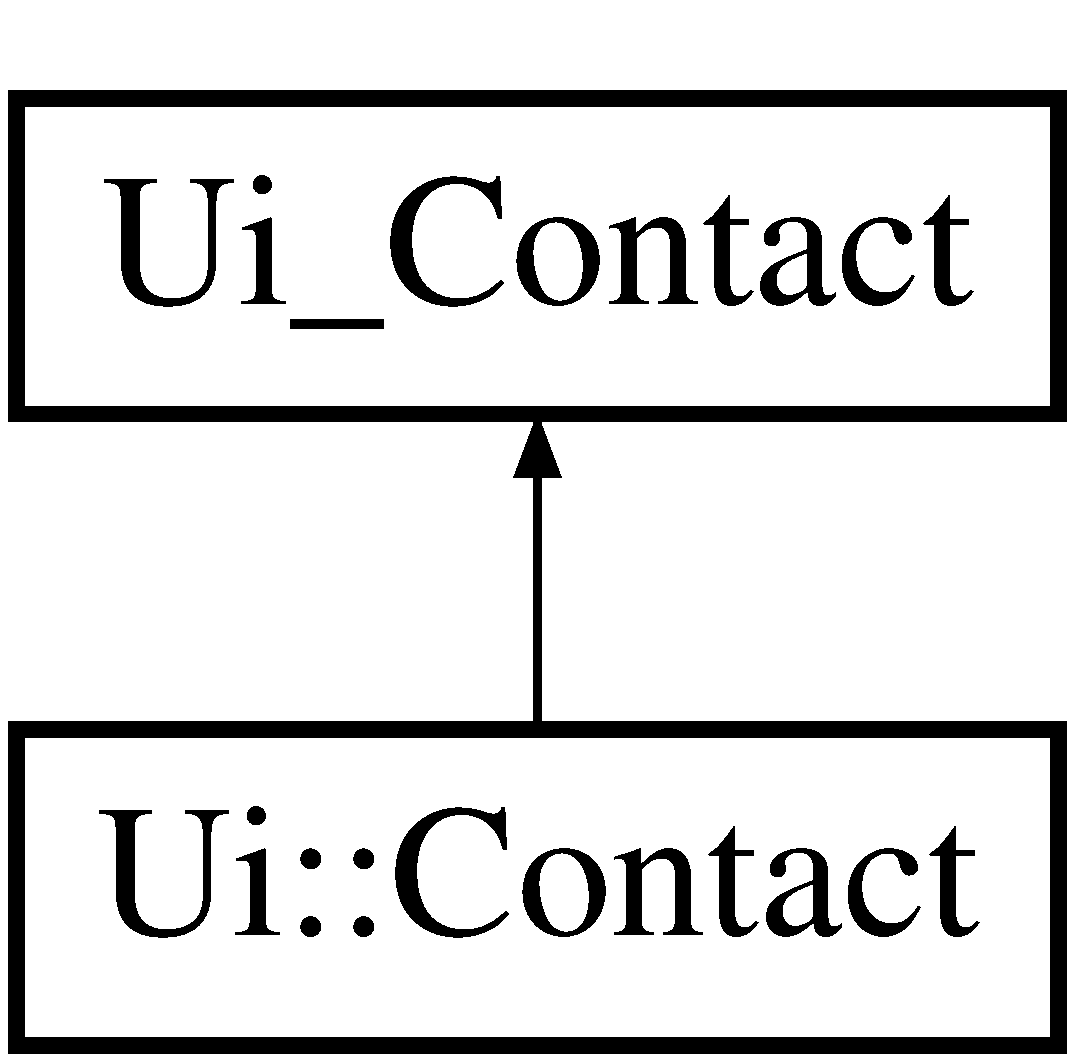
\includegraphics[height=2.000000cm]{class_ui_1_1_contact}
\end{center}
\end{figure}
\subsection*{Additional Inherited Members}


The documentation for this class was generated from the following file\+:\begin{DoxyCompactItemize}
\item 
ui\+\_\+contact.\+h\end{DoxyCompactItemize}

\hypertarget{class_contact}{}\section{Contact Class Reference}
\label{class_contact}\index{Contact@{Contact}}
Inheritance diagram for Contact\+:\begin{figure}[H]
\begin{center}
\leavevmode
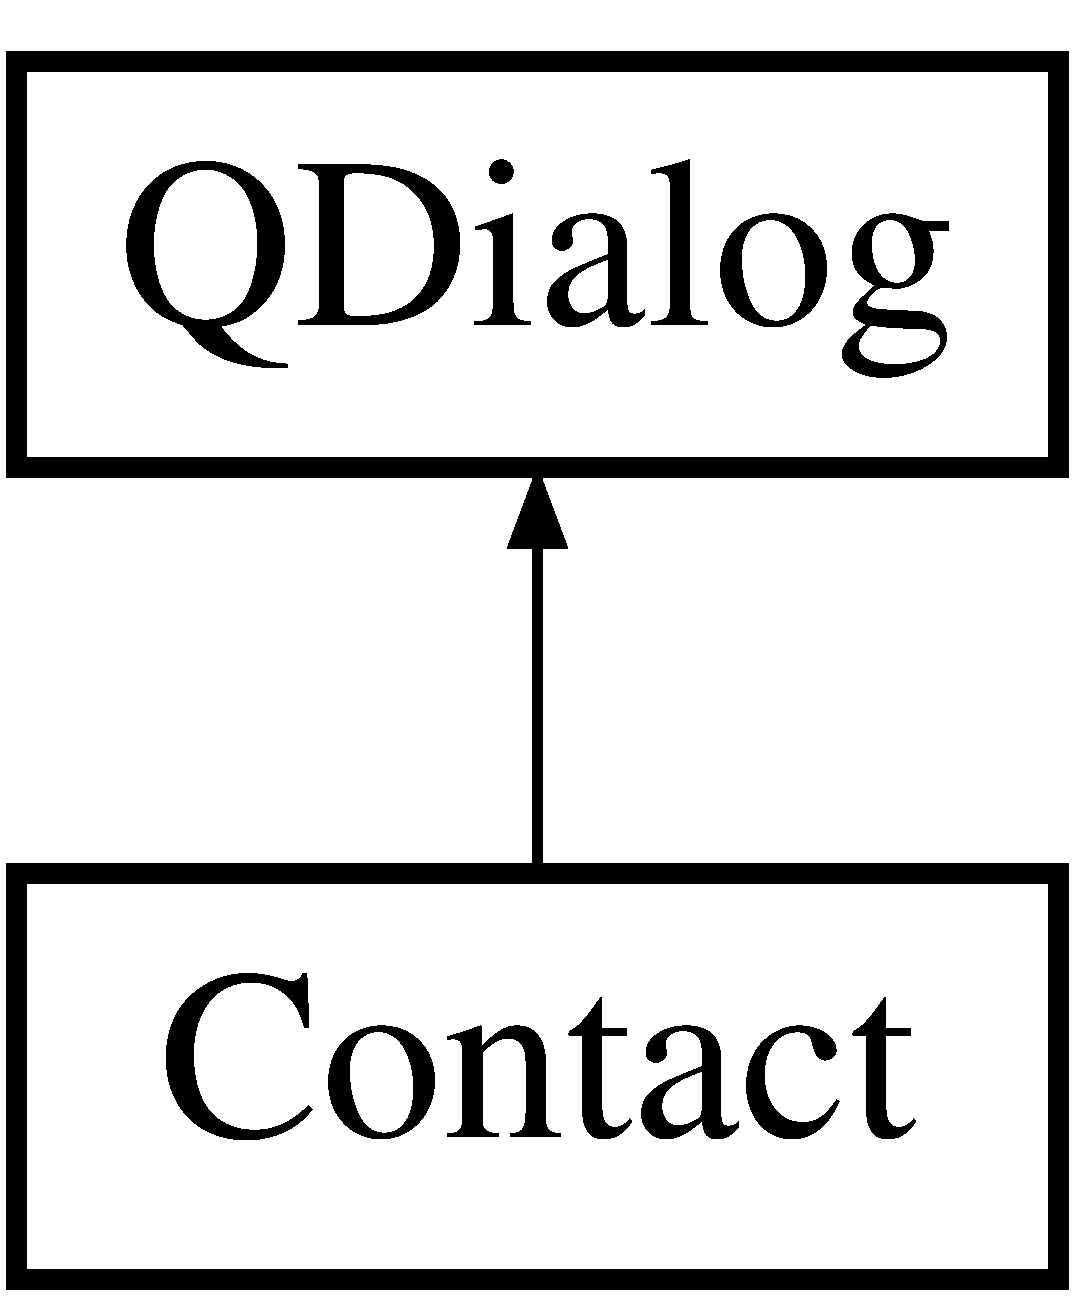
\includegraphics[height=2.000000cm]{class_contact}
\end{center}
\end{figure}
\subsection*{Public Member Functions}
\begin{DoxyCompactItemize}
\item 
\mbox{\Hypertarget{class_contact_a55a5813b1b2a4ddf37634d74152a3fb6}\label{class_contact_a55a5813b1b2a4ddf37634d74152a3fb6}} 
{\bfseries Contact} (Q\+Widget $\ast$parent=0)
\end{DoxyCompactItemize}


The documentation for this class was generated from the following files\+:\begin{DoxyCompactItemize}
\item 
contact.\+h\item 
contact.\+cpp\end{DoxyCompactItemize}

\hypertarget{class_ui_1_1_dialog}{}\section{Ui\+:\+:Dialog Class Reference}
\label{class_ui_1_1_dialog}\index{Ui\+::\+Dialog@{Ui\+::\+Dialog}}
Inheritance diagram for Ui\+:\+:Dialog\+:\begin{figure}[H]
\begin{center}
\leavevmode
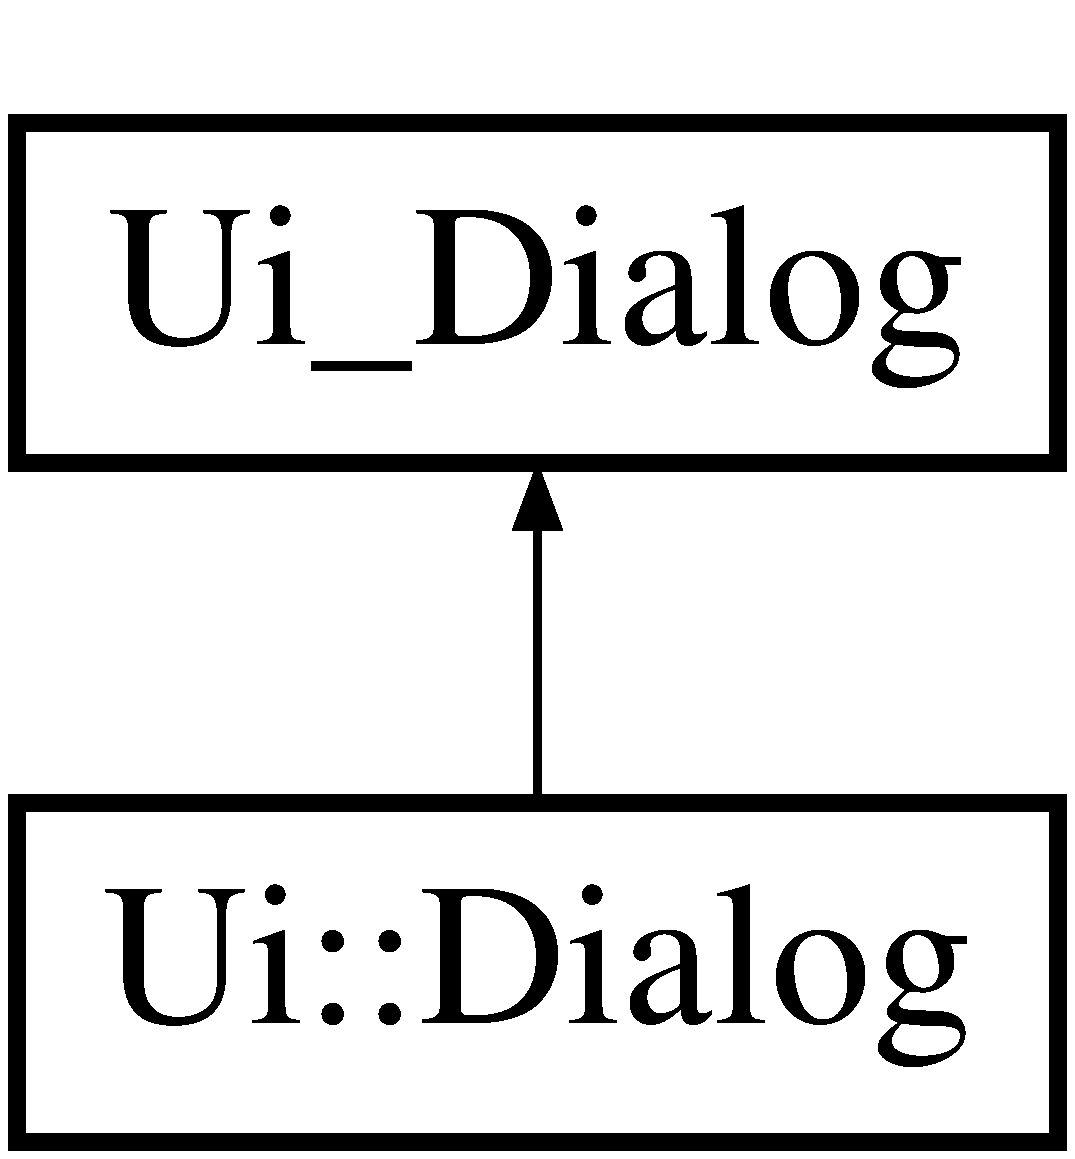
\includegraphics[height=2.000000cm]{class_ui_1_1_dialog}
\end{center}
\end{figure}
\subsection*{Additional Inherited Members}


The documentation for this class was generated from the following file\+:\begin{DoxyCompactItemize}
\item 
ui\+\_\+dialog.\+h\end{DoxyCompactItemize}

\hypertarget{class_ellipse}{}\section{Ellipse Class Reference}
\label{class_ellipse}\index{Ellipse@{Ellipse}}


The \hyperlink{class_ellipse}{Ellipse} class -\/ parent to circle class, handles move functions as well as area and perimeter coming from the virtual base class.  




{\ttfamily \#include $<$Ellipse.\+h$>$}

Inheritance diagram for Ellipse\+:\begin{figure}[H]
\begin{center}
\leavevmode
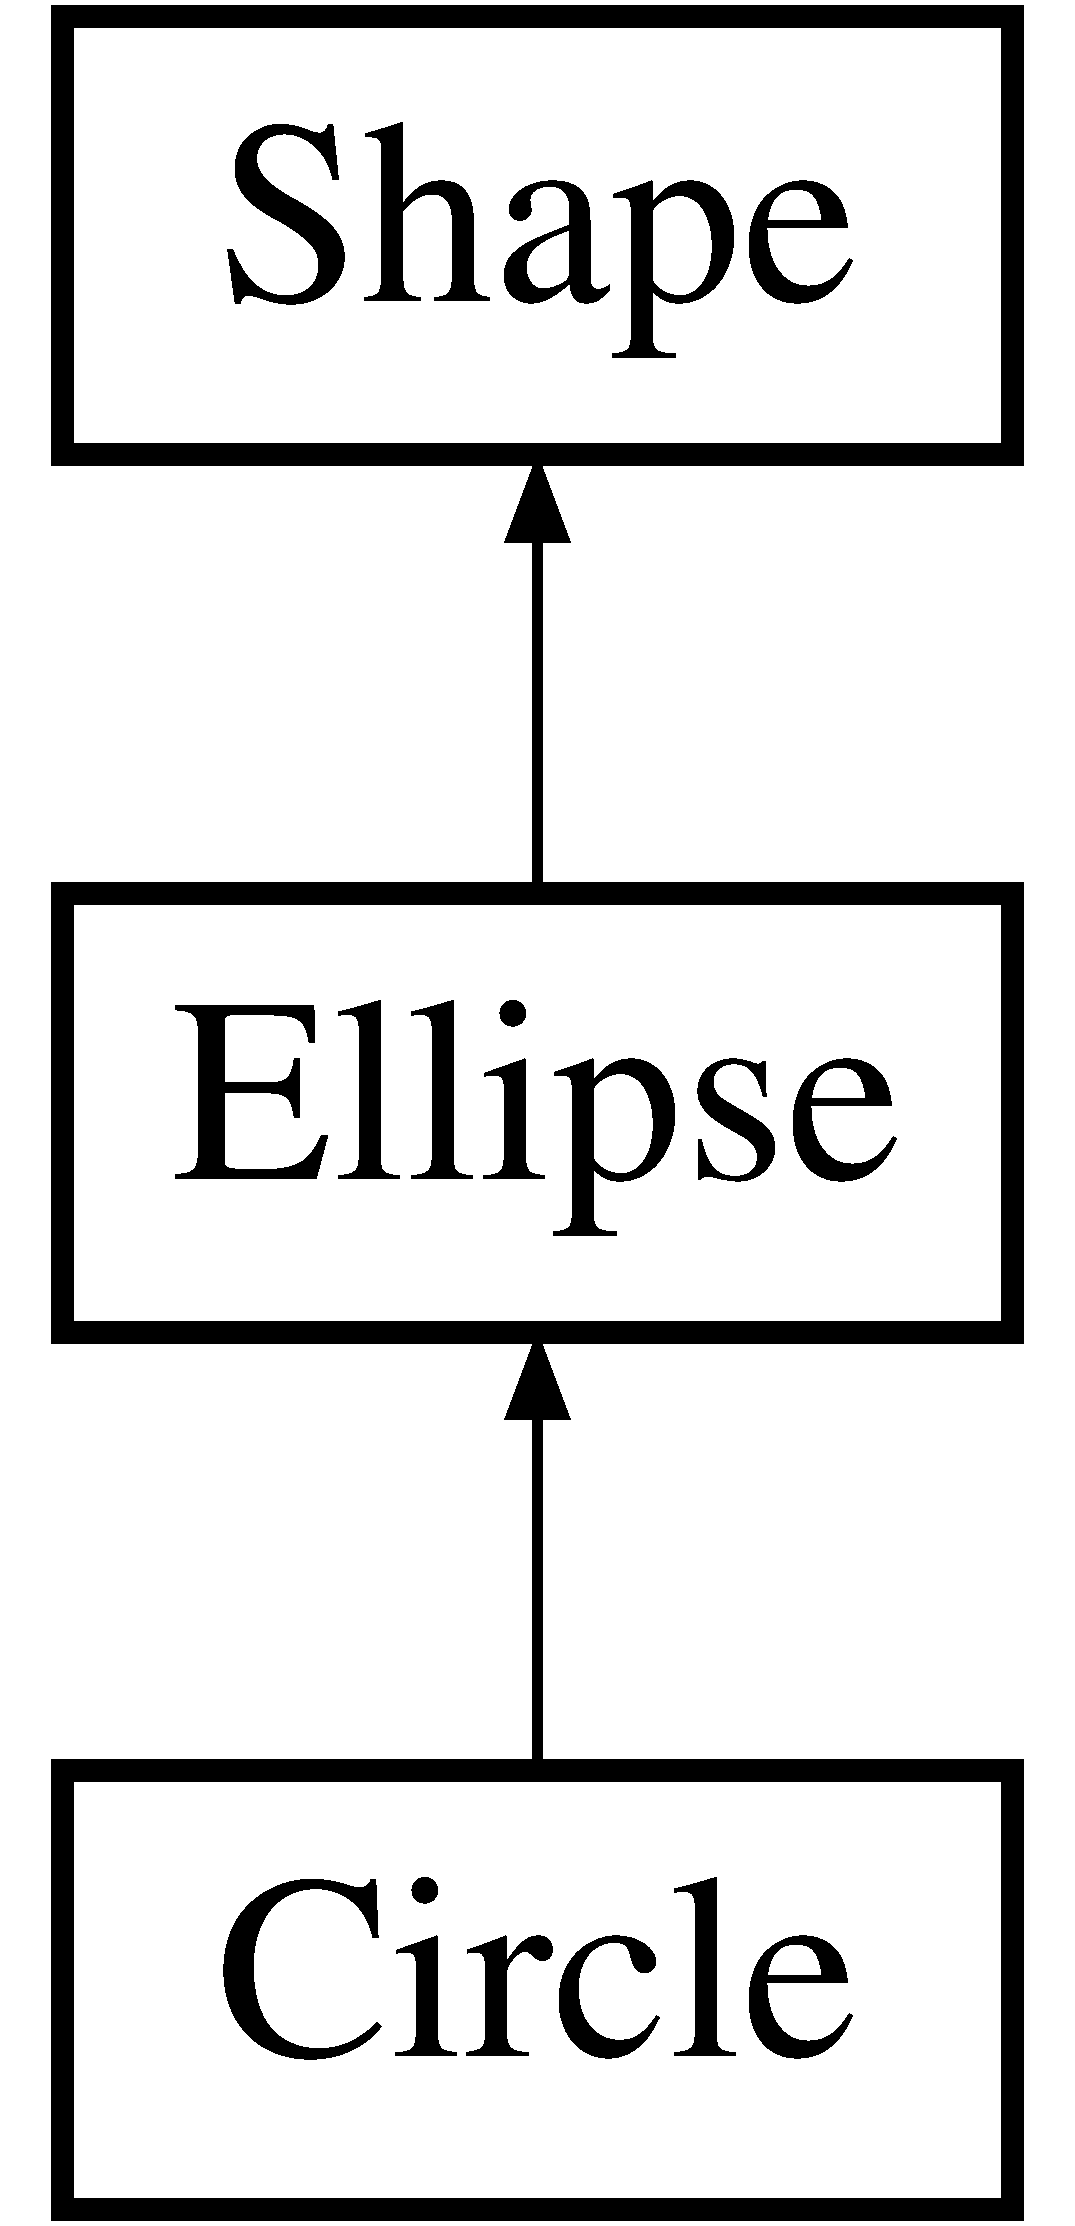
\includegraphics[height=3.000000cm]{class_ellipse}
\end{center}
\end{figure}
\subsection*{Public Member Functions}
\begin{DoxyCompactItemize}
\item 
\mbox{\Hypertarget{class_ellipse_aeb485faf04752402afb7269c04d8c9fc}\label{class_ellipse_aeb485faf04752402afb7269c04d8c9fc}} 
{\bfseries Ellipse} (int x, int y, double xR, double yR)
\item 
\mbox{\Hypertarget{class_ellipse_a0024e8c9f0a3b7dcba13dd463313552b}\label{class_ellipse_a0024e8c9f0a3b7dcba13dd463313552b}} 
{\bfseries Ellipse} (Q\+String id\+In, Qt\+::\+Brush\+Style brush\+Style\+In, Qt\+::\+Global\+Color brush\+Color\+In, double pen\+Width\+In, Qt\+::\+Global\+Color pen\+Color\+In, Qt\+::\+Pen\+Cap\+Style pen\+Cap\+In, Qt\+::\+Pen\+Join\+Style pen\+Join\+In, Qt\+::\+Pen\+Style pen\+Style\+In, double xR, double yR)
\item 
\mbox{\Hypertarget{class_ellipse_a68d1db1ff440a5390c3d2b961095fc90}\label{class_ellipse_a68d1db1ff440a5390c3d2b961095fc90}} 
{\bfseries Ellipse} (\hyperlink{class_ellipse}{Ellipse} \&copy)
\item 
\mbox{\Hypertarget{class_ellipse_a02e36e6e3dc5d7aed93945a960b7a261}\label{class_ellipse_a02e36e6e3dc5d7aed93945a960b7a261}} 
{\bfseries Ellipse} (\hyperlink{class_ellipse}{Ellipse} \&\&copy)
\item 
\mbox{\Hypertarget{class_ellipse_a951f44f301984fac6364ef2746d796c6}\label{class_ellipse_a951f44f301984fac6364ef2746d796c6}} 
virtual void {\bfseries move} (int x\+Des, int y\+Des)
\item 
virtual void \hyperlink{class_ellipse_a8f5c5a4d8051009fee6d861f163c96dd}{move} (Q\+Point xy)
\begin{DoxyCompactList}\small\item\em move -\/ handles moving the shape and recieves in mouse input \end{DoxyCompactList}\item 
\mbox{\Hypertarget{class_ellipse_add1d1c291306985bcbf7cffbebcf4514}\label{class_ellipse_add1d1c291306985bcbf7cffbebcf4514}} 
virtual void {\bfseries Resize} (double radius\+In)
\item 
virtual void \hyperlink{class_ellipse_aaf9524151dc799501327f72c75e0f010}{Draw} (\hyperlink{class_canvas}{Canvas} $\ast$draw\+Area)
\begin{DoxyCompactList}\small\item\em Draw -\/ draws the shape\+: virtual. \end{DoxyCompactList}\item 
\mbox{\Hypertarget{class_ellipse_ad36cbee77639c82f50b763d2b9bbdcf0}\label{class_ellipse_ad36cbee77639c82f50b763d2b9bbdcf0}} 
void {\bfseries SetX} (double x\+In)
\item 
\mbox{\Hypertarget{class_ellipse_a79f8116ec899b31ef5f2281e44b90c1f}\label{class_ellipse_a79f8116ec899b31ef5f2281e44b90c1f}} 
void {\bfseries SetY} (double y\+In)
\item 
\mbox{\Hypertarget{class_ellipse_a3b6a92ab290475f2c6eb5a930b31d741}\label{class_ellipse_a3b6a92ab290475f2c6eb5a930b31d741}} 
double {\bfseries get\+Area} ()
\item 
\mbox{\Hypertarget{class_ellipse_a6b5ac7a4f1e68f9c5a66f0d8d66acc3c}\label{class_ellipse_a6b5ac7a4f1e68f9c5a66f0d8d66acc3c}} 
double {\bfseries get\+Perimeter} ()
\item 
virtual bool \hyperlink{class_ellipse_ab3ba6c9f068fc37808778c74f1273f69}{is\+\_\+\+Left\+\_\+\+Clicked} (Q\+Point xy)
\begin{DoxyCompactList}\small\item\em is\+\_\+\+Left\+\_\+\+Clicked -\/ mouse input \end{DoxyCompactList}\item 
\mbox{\Hypertarget{class_ellipse_a8382720255d2a9625e3d785324d2f9f7}\label{class_ellipse_a8382720255d2a9625e3d785324d2f9f7}} 
virtual void {\bfseries say\+Hi} ()
\end{DoxyCompactItemize}
\subsection*{Protected Attributes}
\begin{DoxyCompactItemize}
\item 
\mbox{\Hypertarget{class_ellipse_a70771f8c320a2ae285a04fa97e808ff0}\label{class_ellipse_a70771f8c320a2ae285a04fa97e808ff0}} 
int {\bfseries x}
\item 
\mbox{\Hypertarget{class_ellipse_a37ca7f50a9df28e00428077cc1a38a3a}\label{class_ellipse_a37ca7f50a9df28e00428077cc1a38a3a}} 
int {\bfseries y}
\item 
\mbox{\Hypertarget{class_ellipse_a8e0e2fa0f3200a997f4b0567e588c823}\label{class_ellipse_a8e0e2fa0f3200a997f4b0567e588c823}} 
double {\bfseries x\+Radius}
\item 
\mbox{\Hypertarget{class_ellipse_a83614d1aaa446b1f8e404b6bc3cc8c19}\label{class_ellipse_a83614d1aaa446b1f8e404b6bc3cc8c19}} 
double {\bfseries y\+Radius}
\item 
\mbox{\Hypertarget{class_ellipse_af632e808976bdd5598bbae897cc359d7}\label{class_ellipse_af632e808976bdd5598bbae897cc359d7}} 
const double {\bfseries pi} = 3.\+14159265359
\end{DoxyCompactItemize}
\subsection*{Static Protected Attributes}
\begin{DoxyCompactItemize}
\item 
\mbox{\Hypertarget{class_ellipse_ad58a3d79058ccc3a31b3fc6bc6cd9a30}\label{class_ellipse_ad58a3d79058ccc3a31b3fc6bc6cd9a30}} 
static int {\bfseries ellipse\+Counter}
\end{DoxyCompactItemize}


\subsection{Detailed Description}
The \hyperlink{class_ellipse}{Ellipse} class -\/ parent to circle class, handles move functions as well as area and perimeter coming from the virtual base class. 

\subsection{Member Function Documentation}
\mbox{\Hypertarget{class_ellipse_aaf9524151dc799501327f72c75e0f010}\label{class_ellipse_aaf9524151dc799501327f72c75e0f010}} 
\index{Ellipse@{Ellipse}!Draw@{Draw}}
\index{Draw@{Draw}!Ellipse@{Ellipse}}
\subsubsection{\texorpdfstring{Draw()}{Draw()}}
{\footnotesize\ttfamily void Ellipse\+::\+Draw (\begin{DoxyParamCaption}\item[{\hyperlink{class_canvas}{Canvas} $\ast$}]{paint\+Area }\end{DoxyParamCaption})\hspace{0.3cm}{\ttfamily [virtual]}}



Draw -\/ draws the shape\+: virtual. 


\begin{DoxyParams}{Parameters}
{\em paint\+Area} & \\
\hline
\end{DoxyParams}


Reimplemented from \hyperlink{class_shape_ad7cc6a5e97b0971d50999bce4396127a}{Shape}.



Reimplemented in \hyperlink{class_circle_a5bebd94955572edce0ad10208a449772}{Circle}.

\mbox{\Hypertarget{class_ellipse_ab3ba6c9f068fc37808778c74f1273f69}\label{class_ellipse_ab3ba6c9f068fc37808778c74f1273f69}} 
\index{Ellipse@{Ellipse}!is\+\_\+\+Left\+\_\+\+Clicked@{is\+\_\+\+Left\+\_\+\+Clicked}}
\index{is\+\_\+\+Left\+\_\+\+Clicked@{is\+\_\+\+Left\+\_\+\+Clicked}!Ellipse@{Ellipse}}
\subsubsection{\texorpdfstring{is\+\_\+\+Left\+\_\+\+Clicked()}{is\_Left\_Clicked()}}
{\footnotesize\ttfamily bool Ellipse\+::is\+\_\+\+Left\+\_\+\+Clicked (\begin{DoxyParamCaption}\item[{Q\+Point}]{e }\end{DoxyParamCaption})\hspace{0.3cm}{\ttfamily [virtual]}}



is\+\_\+\+Left\+\_\+\+Clicked -\/ mouse input 


\begin{DoxyParams}{Parameters}
{\em e} & \\
\hline
\end{DoxyParams}
\begin{DoxyReturn}{Returns}

\end{DoxyReturn}


Reimplemented from \hyperlink{class_shape_ab2d47c913eb287843e61b2d48e422ced}{Shape}.



Reimplemented in \hyperlink{class_circle_a1661bb4e324cce0196a6aa1195c26c73}{Circle}.

\mbox{\Hypertarget{class_ellipse_a8f5c5a4d8051009fee6d861f163c96dd}\label{class_ellipse_a8f5c5a4d8051009fee6d861f163c96dd}} 
\index{Ellipse@{Ellipse}!move@{move}}
\index{move@{move}!Ellipse@{Ellipse}}
\subsubsection{\texorpdfstring{move()}{move()}}
{\footnotesize\ttfamily void Ellipse\+::move (\begin{DoxyParamCaption}\item[{Q\+Point}]{xy }\end{DoxyParamCaption})\hspace{0.3cm}{\ttfamily [virtual]}}



move -\/ handles moving the shape and recieves in mouse input 


\begin{DoxyParams}{Parameters}
{\em xy} & \\
\hline
\end{DoxyParams}


Reimplemented from \hyperlink{class_shape_a26d57a0589b0fd7ff03a4b5ad8dc530a}{Shape}.



Reimplemented in \hyperlink{class_circle_a5f02de3ad7e992a689b9f9e88643076c}{Circle}.



The documentation for this class was generated from the following files\+:\begin{DoxyCompactItemize}
\item 
Ellipse.\+h\item 
Ellipse.\+cpp\end{DoxyCompactItemize}

\hypertarget{class_help}{}\section{Help Class Reference}
\label{class_help}\index{Help@{Help}}
Inheritance diagram for Help\+:\begin{figure}[H]
\begin{center}
\leavevmode
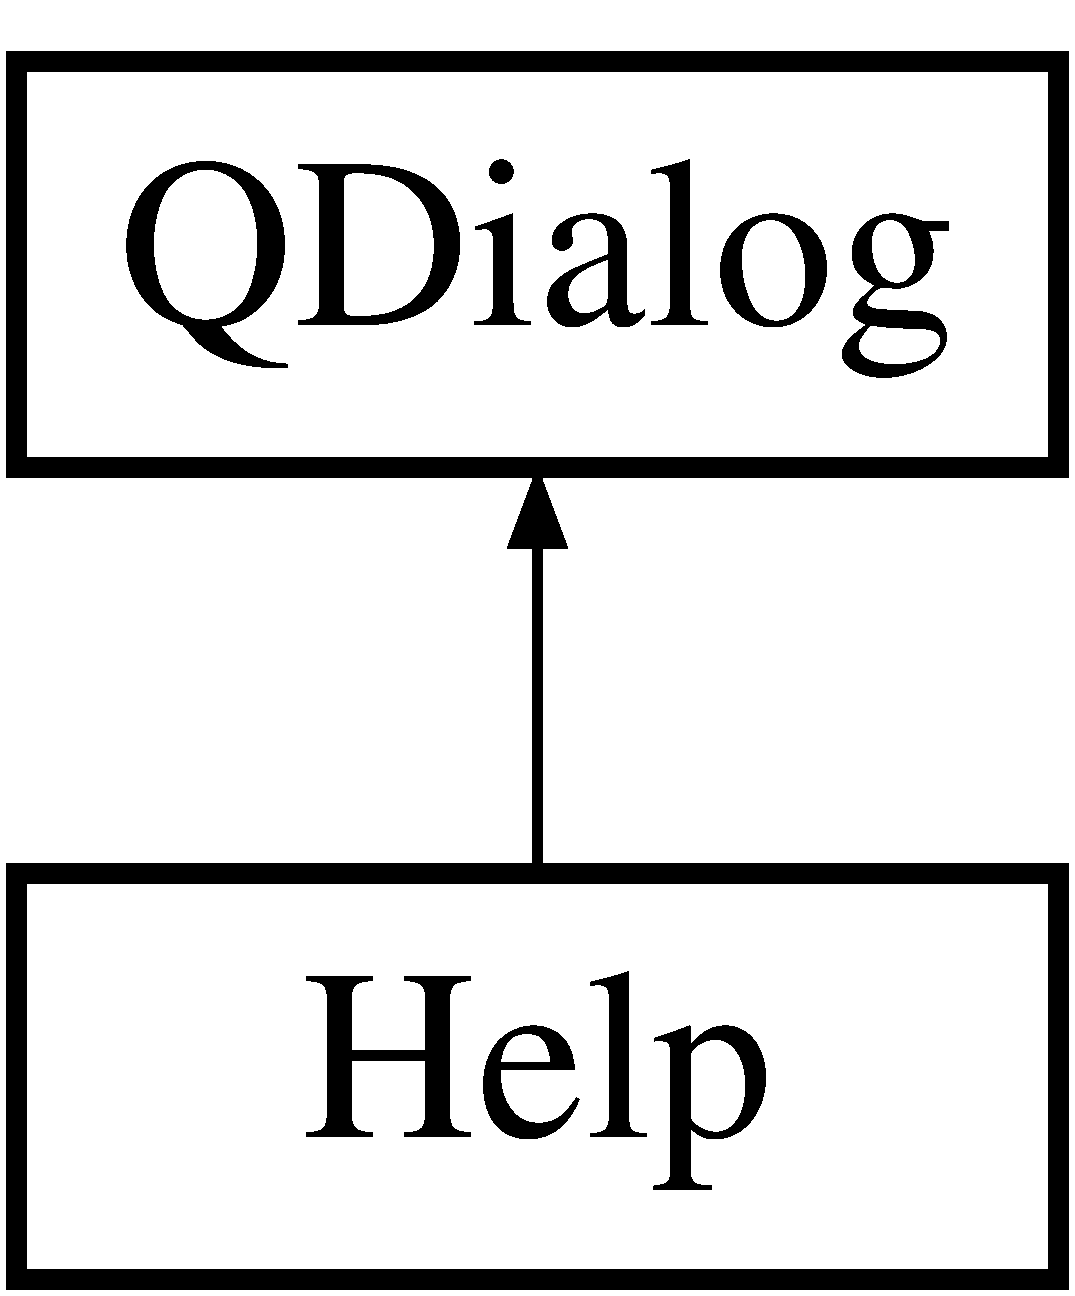
\includegraphics[height=2.000000cm]{class_help}
\end{center}
\end{figure}
\subsection*{Public Member Functions}
\begin{DoxyCompactItemize}
\item 
\mbox{\Hypertarget{class_help_a7359f816eb2dab34e4c7017e36c9654d}\label{class_help_a7359f816eb2dab34e4c7017e36c9654d}} 
{\bfseries Help} (Q\+Widget $\ast$parent=0)
\end{DoxyCompactItemize}


The documentation for this class was generated from the following files\+:\begin{DoxyCompactItemize}
\item 
help.\+h\item 
help.\+cpp\end{DoxyCompactItemize}

\hypertarget{class_ui_1_1_help}{}\section{Ui\+:\+:Help Class Reference}
\label{class_ui_1_1_help}\index{Ui\+::\+Help@{Ui\+::\+Help}}
Inheritance diagram for Ui\+:\+:Help\+:\begin{figure}[H]
\begin{center}
\leavevmode
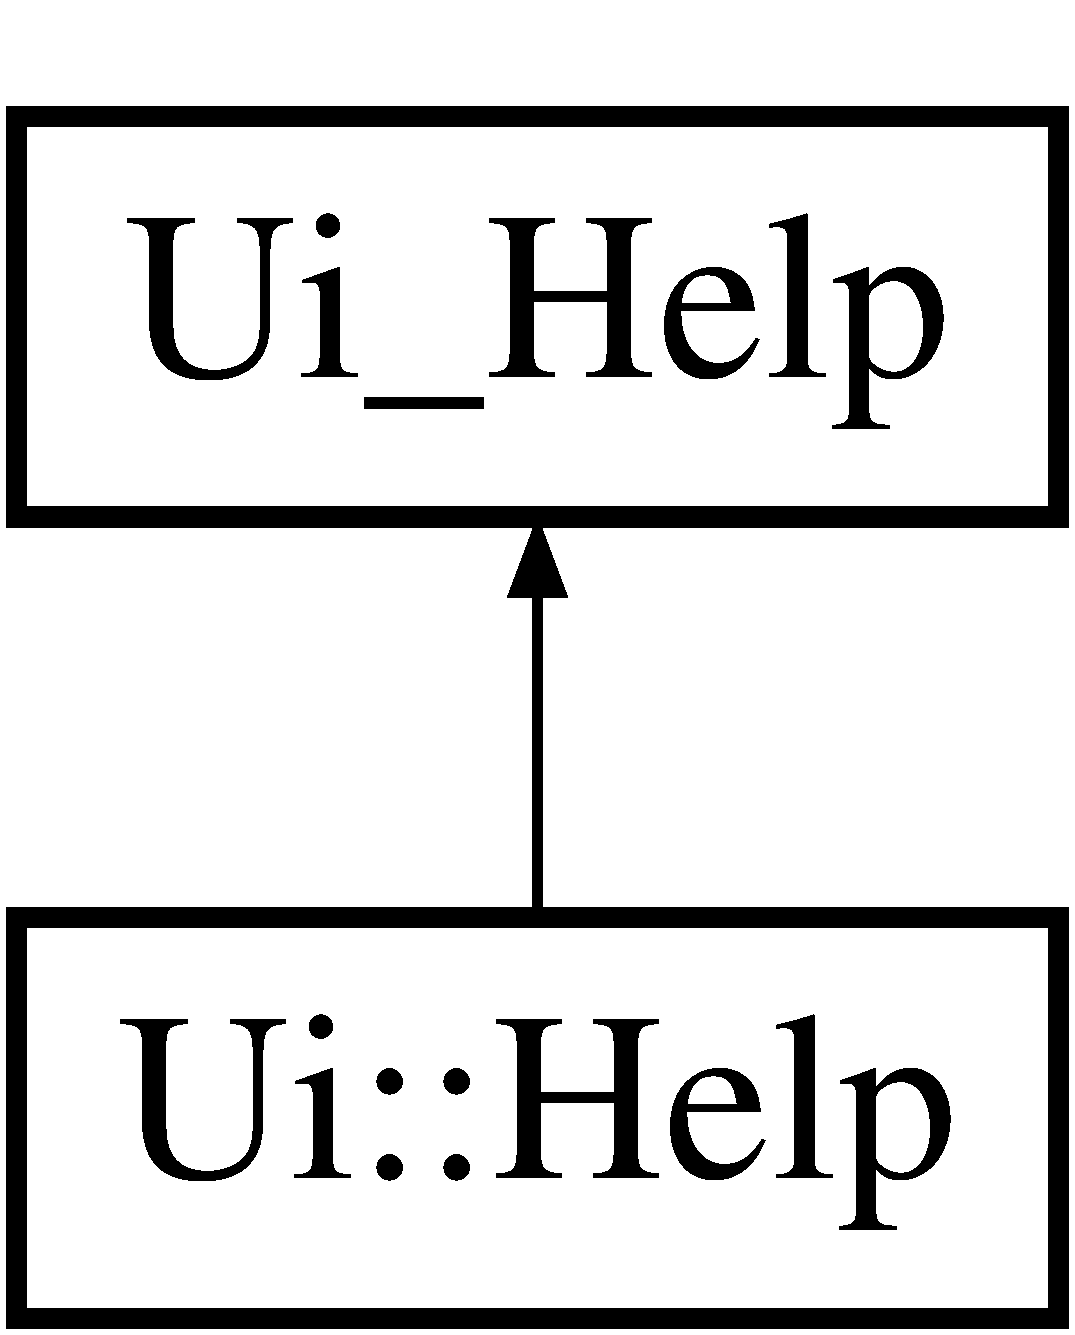
\includegraphics[height=2.000000cm]{class_ui_1_1_help}
\end{center}
\end{figure}
\subsection*{Additional Inherited Members}


The documentation for this class was generated from the following file\+:\begin{DoxyCompactItemize}
\item 
ui\+\_\+help.\+h\end{DoxyCompactItemize}

\hypertarget{class_line}{}\section{Line Class Reference}
\label{class_line}\index{Line@{Line}}


The \hyperlink{class_line}{Line} class -\/ derived from the abstarct shape class\+: can manipulate all of the pen and brush styles and colors.  




{\ttfamily \#include $<$Line.\+h$>$}

Inheritance diagram for Line\+:\begin{figure}[H]
\begin{center}
\leavevmode
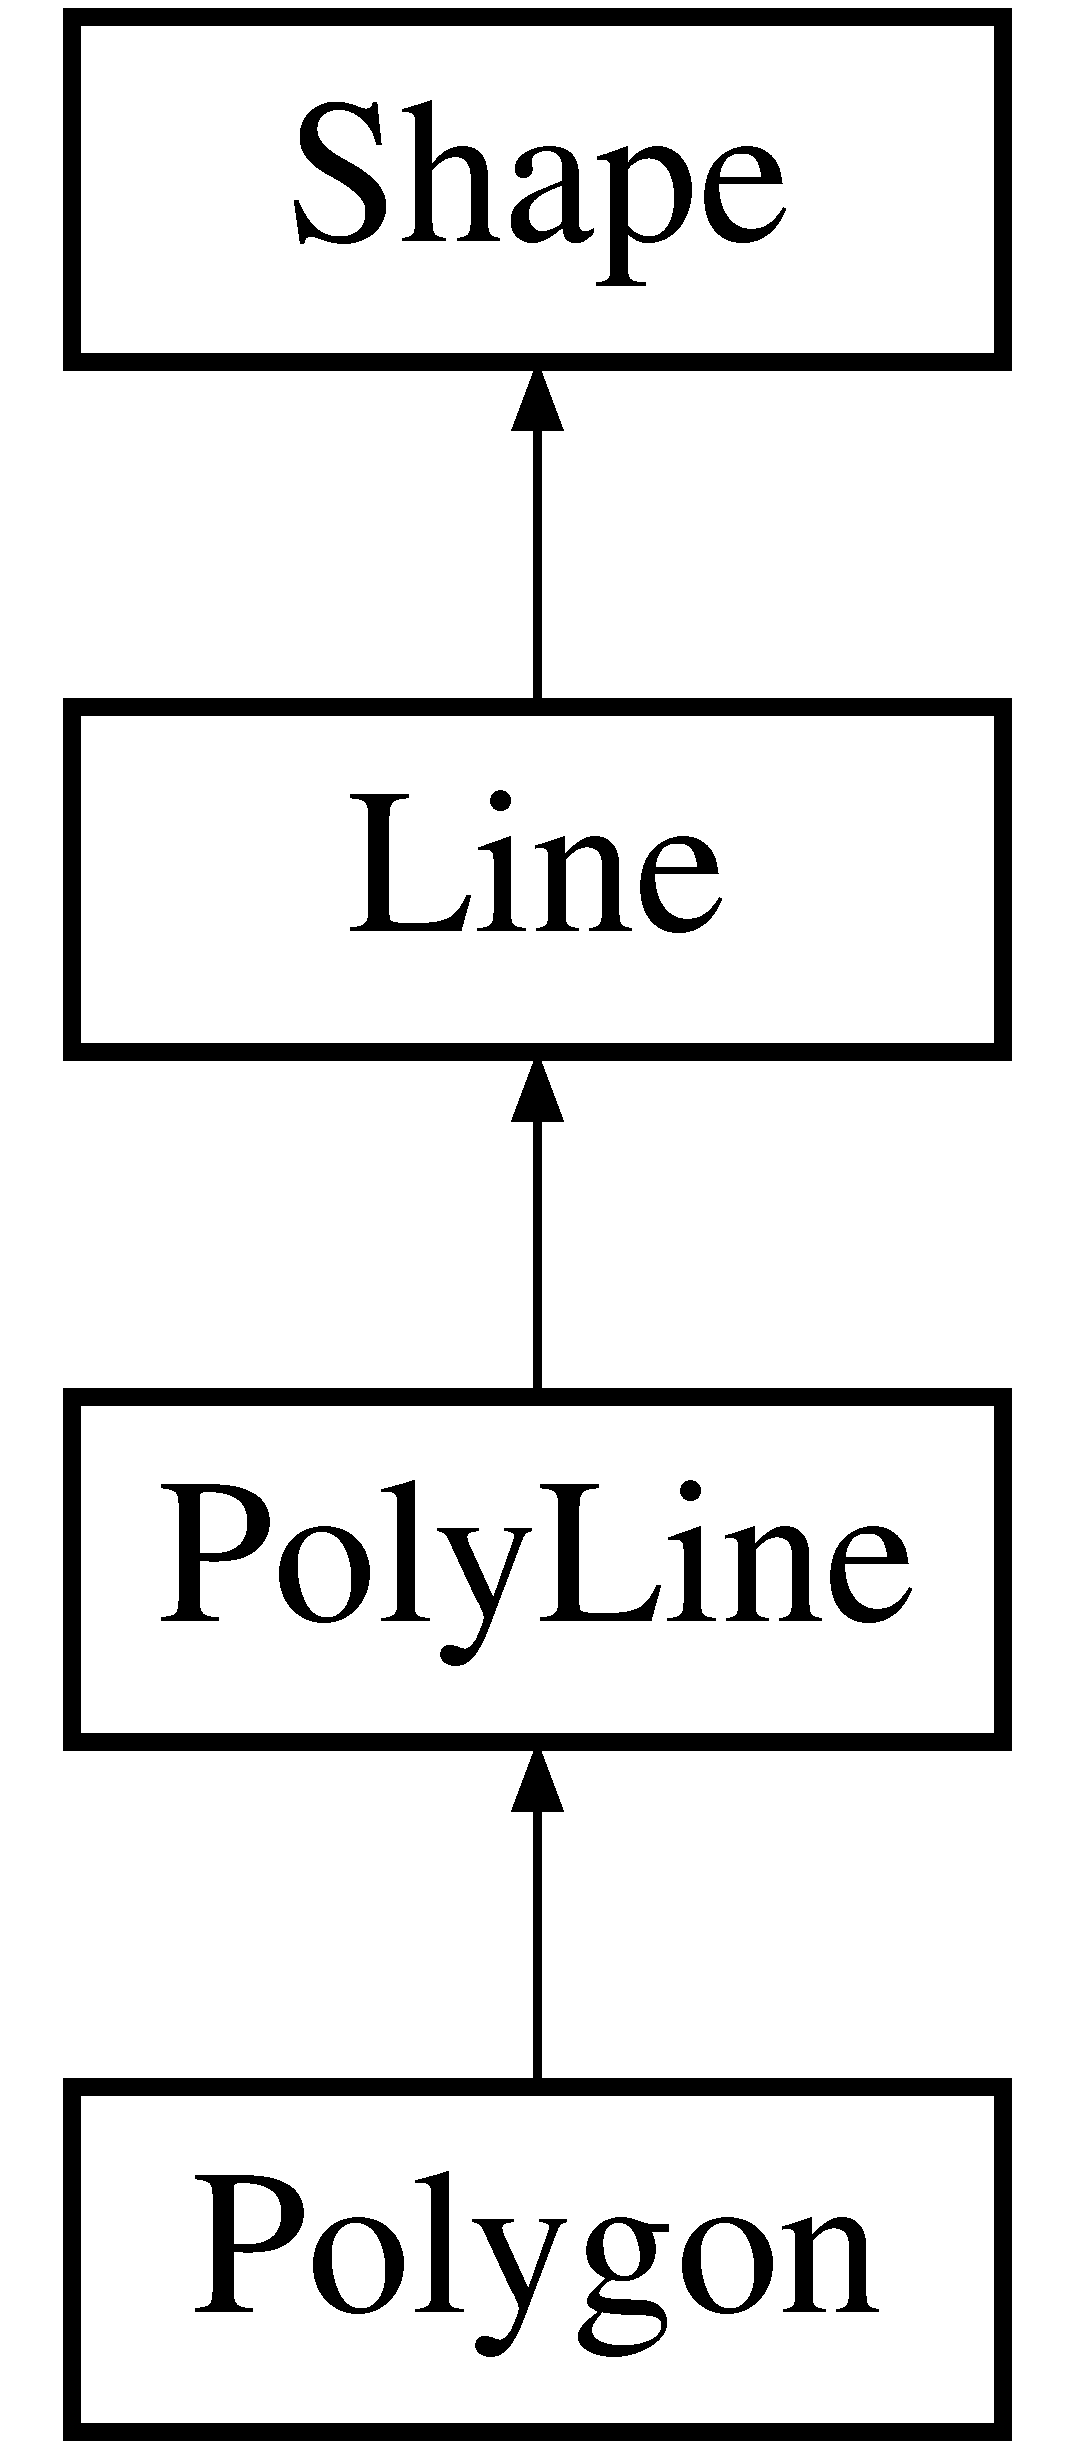
\includegraphics[height=4.000000cm]{class_line}
\end{center}
\end{figure}
\subsection*{Public Member Functions}
\begin{DoxyCompactItemize}
\item 
\mbox{\Hypertarget{class_line_abad71cdf25c42d0794814bbfb4a21db8}\label{class_line_abad71cdf25c42d0794814bbfb4a21db8}} 
{\bfseries Line} (Q\+Polygon e)
\item 
\mbox{\Hypertarget{class_line_ae007adde85949ea26e74987d09a7c3e5}\label{class_line_ae007adde85949ea26e74987d09a7c3e5}} 
{\bfseries Line} (Q\+String id\+In, Qt\+::\+Brush\+Style brush\+Style\+In, Qt\+::\+Global\+Color brush\+Color\+In, double pen\+Width\+In, Qt\+::\+Global\+Color pen\+Color\+In, Qt\+::\+Pen\+Cap\+Style pen\+Cap\+In, Qt\+::\+Pen\+Join\+Style pen\+Join\+In, Qt\+::\+Pen\+Style pen\+Style\+In, int x, int y)
\item 
\mbox{\Hypertarget{class_line_abf6160ef558a50fab058f2e33561a102}\label{class_line_abf6160ef558a50fab058f2e33561a102}} 
{\bfseries Line} (Q\+String id\+In, Qt\+::\+Brush\+Style brush\+Style\+In, Qt\+::\+Global\+Color brush\+Color\+In, double pen\+Width\+In, Qt\+::\+Global\+Color pen\+Color\+In, Qt\+::\+Pen\+Cap\+Style pen\+Cap\+In, Qt\+::\+Pen\+Join\+Style pen\+Join\+In, Qt\+::\+Pen\+Style pen\+Style\+In)
\item 
virtual void \hyperlink{class_line_a01ac38eae66f157868daee1b4764b242}{push\+\_\+\+Back\+\_\+point} (Q\+Point e)
\begin{DoxyCompactList}\small\item\em push\+\_\+\+Back\+\_\+point -\/ how the line is actually created, pushing back two points will tell the canvas where exactly to construct the line and where to stop based off of mouse input \end{DoxyCompactList}\item 
\mbox{\Hypertarget{class_line_a7f82d921d86db81eea79bd4f8452024c}\label{class_line_a7f82d921d86db81eea79bd4f8452024c}} 
virtual void {\bfseries push\+\_\+\+Back\+\_\+point} (int x, int y)
\item 
\mbox{\Hypertarget{class_line_af882f56947a1c83eaac5ce1d9e0088a8}\label{class_line_af882f56947a1c83eaac5ce1d9e0088a8}} 
virtual void {\bfseries move\+Last\+Point} (Q\+Point e)
\item 
virtual void \hyperlink{class_line_ae645f8a7f03439fa3428f81b1ddb4ffc}{Draw} (\hyperlink{class_canvas}{Canvas} $\ast$draw\+Area)
\begin{DoxyCompactList}\small\item\em Draw -\/ draws the shape\+: virtual. \end{DoxyCompactList}\item 
virtual bool \hyperlink{class_line_a79c3891fefd740e6a3cfcdb57a105995}{is\+\_\+\+Left\+\_\+\+Clicked} (Q\+Point e)
\begin{DoxyCompactList}\small\item\em is\+\_\+\+Left\+\_\+\+Clicked -\/ mouse input \end{DoxyCompactList}\item 
\mbox{\Hypertarget{class_line_ad0e0cc191a40c9203e6e8f753d837f01}\label{class_line_ad0e0cc191a40c9203e6e8f753d837f01}} 
int {\bfseries get\+Pointnum} ()
\end{DoxyCompactItemize}
\subsection*{Protected Attributes}
\begin{DoxyCompactItemize}
\item 
\mbox{\Hypertarget{class_line_acb42aa5b881c81224994fdcd80227e73}\label{class_line_acb42aa5b881c81224994fdcd80227e73}} 
Q\+Polygon {\bfseries points}
\item 
\mbox{\Hypertarget{class_line_a0954f1ba173e19a23eb88b3c56d59c04}\label{class_line_a0954f1ba173e19a23eb88b3c56d59c04}} 
int {\bfseries point\+\_\+counter}
\end{DoxyCompactItemize}


\subsection{Detailed Description}
The \hyperlink{class_line}{Line} class -\/ derived from the abstarct shape class\+: can manipulate all of the pen and brush styles and colors. 

\subsection{Member Function Documentation}
\mbox{\Hypertarget{class_line_ae645f8a7f03439fa3428f81b1ddb4ffc}\label{class_line_ae645f8a7f03439fa3428f81b1ddb4ffc}} 
\index{Line@{Line}!Draw@{Draw}}
\index{Draw@{Draw}!Line@{Line}}
\subsubsection{\texorpdfstring{Draw()}{Draw()}}
{\footnotesize\ttfamily void Line\+::\+Draw (\begin{DoxyParamCaption}\item[{\hyperlink{class_canvas}{Canvas} $\ast$}]{paint\+Area }\end{DoxyParamCaption})\hspace{0.3cm}{\ttfamily [virtual]}}



Draw -\/ draws the shape\+: virtual. 


\begin{DoxyParams}{Parameters}
{\em paint\+Area} & \\
\hline
\end{DoxyParams}


Reimplemented from \hyperlink{class_shape_ad7cc6a5e97b0971d50999bce4396127a}{Shape}.



Reimplemented in \hyperlink{class_polygon_a9271921d96331c203efcdb50e0ebd64c}{Polygon}, and \hyperlink{class_poly_line_ac42ca364849f33b899a929bf57163730}{Poly\+Line}.

\mbox{\Hypertarget{class_line_a79c3891fefd740e6a3cfcdb57a105995}\label{class_line_a79c3891fefd740e6a3cfcdb57a105995}} 
\index{Line@{Line}!is\+\_\+\+Left\+\_\+\+Clicked@{is\+\_\+\+Left\+\_\+\+Clicked}}
\index{is\+\_\+\+Left\+\_\+\+Clicked@{is\+\_\+\+Left\+\_\+\+Clicked}!Line@{Line}}
\subsubsection{\texorpdfstring{is\+\_\+\+Left\+\_\+\+Clicked()}{is\_Left\_Clicked()}}
{\footnotesize\ttfamily bool Line\+::is\+\_\+\+Left\+\_\+\+Clicked (\begin{DoxyParamCaption}\item[{Q\+Point}]{e }\end{DoxyParamCaption})\hspace{0.3cm}{\ttfamily [virtual]}}



is\+\_\+\+Left\+\_\+\+Clicked -\/ mouse input 


\begin{DoxyParams}{Parameters}
{\em e} & \\
\hline
\end{DoxyParams}
\begin{DoxyReturn}{Returns}

\end{DoxyReturn}


Reimplemented from \hyperlink{class_shape_ab2d47c913eb287843e61b2d48e422ced}{Shape}.



Reimplemented in \hyperlink{class_polygon_ab17f2f8ae9489fba4030fbb4a99e7ea6}{Polygon}, and \hyperlink{class_poly_line_a349f5b14d3ab568ae6776a3d5fd6f956}{Poly\+Line}.

\mbox{\Hypertarget{class_line_a01ac38eae66f157868daee1b4764b242}\label{class_line_a01ac38eae66f157868daee1b4764b242}} 
\index{Line@{Line}!push\+\_\+\+Back\+\_\+point@{push\+\_\+\+Back\+\_\+point}}
\index{push\+\_\+\+Back\+\_\+point@{push\+\_\+\+Back\+\_\+point}!Line@{Line}}
\subsubsection{\texorpdfstring{push\+\_\+\+Back\+\_\+point()}{push\_Back\_point()}}
{\footnotesize\ttfamily void Line\+::push\+\_\+\+Back\+\_\+point (\begin{DoxyParamCaption}\item[{Q\+Point}]{e }\end{DoxyParamCaption})\hspace{0.3cm}{\ttfamily [virtual]}}



push\+\_\+\+Back\+\_\+point -\/ how the line is actually created, pushing back two points will tell the canvas where exactly to construct the line and where to stop based off of mouse input 


\begin{DoxyParams}{Parameters}
{\em e} & \\
\hline
\end{DoxyParams}


Reimplemented in \hyperlink{class_polygon_ad57f4b375c6858bfe34c095bfeb38d5a}{Polygon}, and \hyperlink{class_poly_line_afbc3a0e59abcd27bdb58027796e91c3a}{Poly\+Line}.



The documentation for this class was generated from the following files\+:\begin{DoxyCompactItemize}
\item 
Line.\+h\item 
line.\+cpp\end{DoxyCompactItemize}

\hypertarget{class_ui_1_1_login_screen}{}\section{Ui\+:\+:Login\+Screen Class Reference}
\label{class_ui_1_1_login_screen}\index{Ui\+::\+Login\+Screen@{Ui\+::\+Login\+Screen}}
Inheritance diagram for Ui\+:\+:Login\+Screen\+:\begin{figure}[H]
\begin{center}
\leavevmode
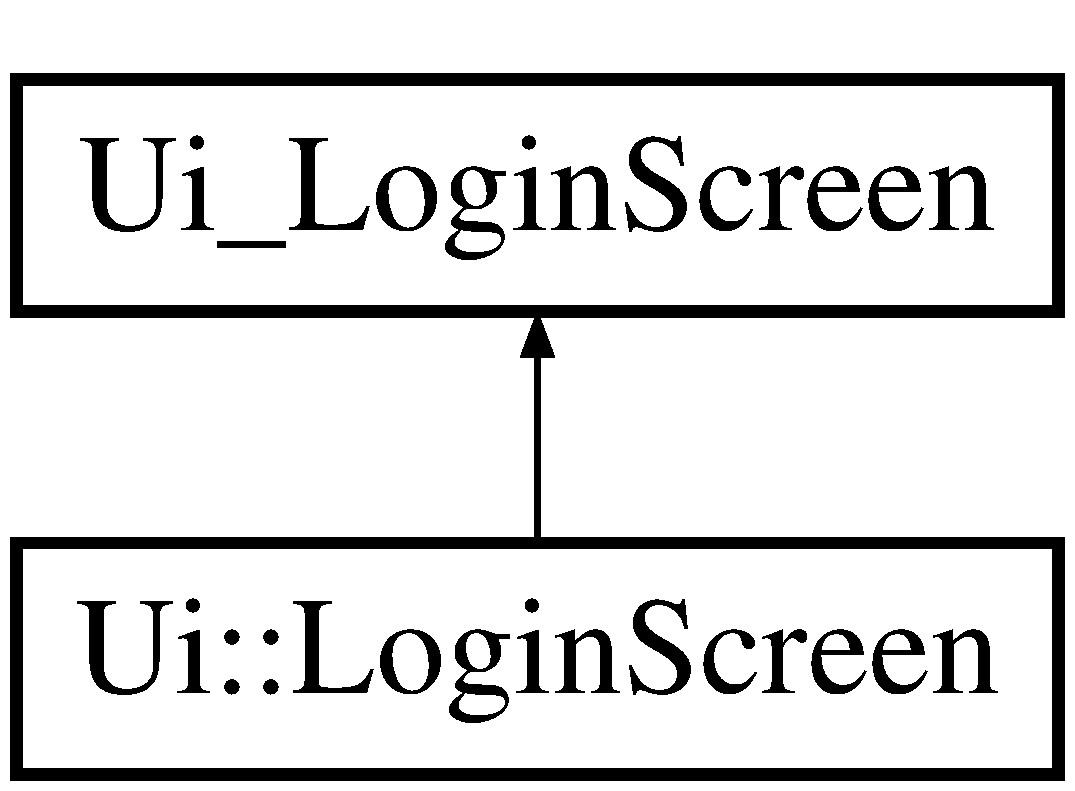
\includegraphics[height=2.000000cm]{class_ui_1_1_login_screen}
\end{center}
\end{figure}
\subsection*{Additional Inherited Members}


The documentation for this class was generated from the following file\+:\begin{DoxyCompactItemize}
\item 
ui\+\_\+loginscreen.\+h\end{DoxyCompactItemize}

\hypertarget{class_login_screen}{}\section{Login\+Screen Class Reference}
\label{class_login_screen}\index{Login\+Screen@{Login\+Screen}}


The \hyperlink{class_login_screen}{Login\+Screen} class -\/ obsolete\+:replaced by newnew.\+ui.  




{\ttfamily \#include $<$loginscreen.\+h$>$}

Inheritance diagram for Login\+Screen\+:\begin{figure}[H]
\begin{center}
\leavevmode
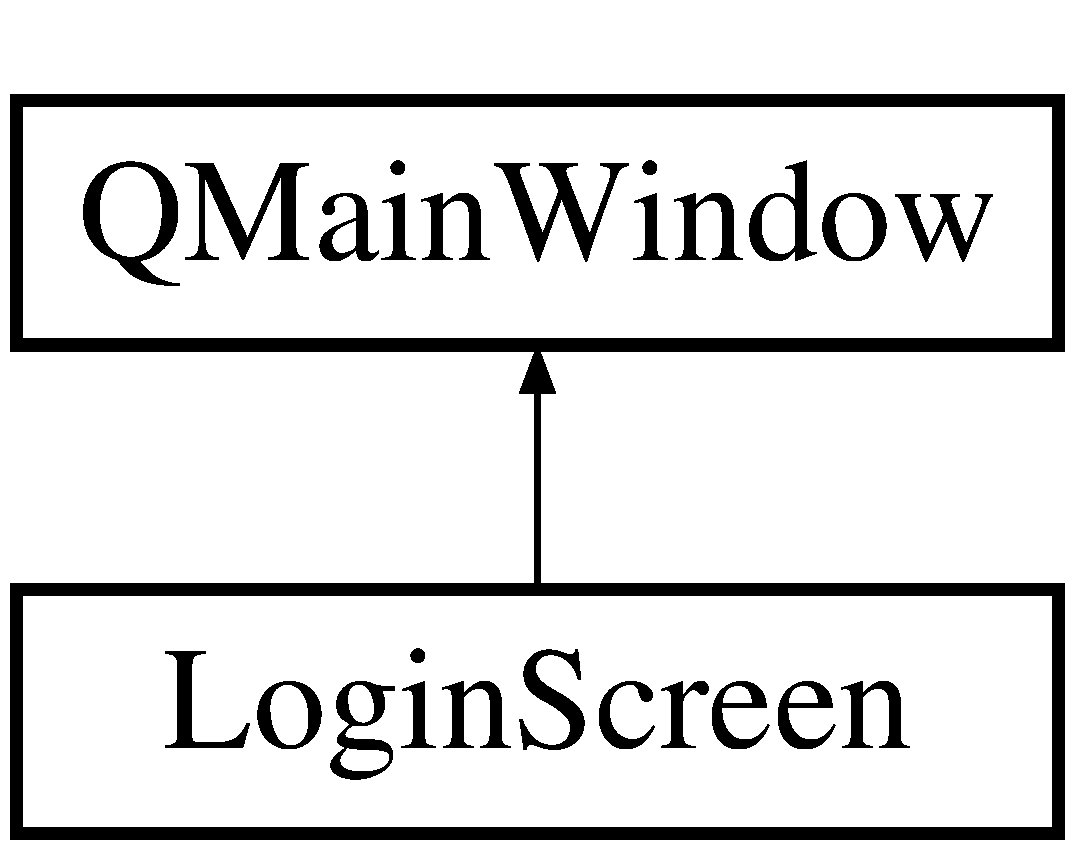
\includegraphics[height=2.000000cm]{class_login_screen}
\end{center}
\end{figure}
\subsection*{Public Member Functions}
\begin{DoxyCompactItemize}
\item 
\mbox{\Hypertarget{class_login_screen_a1ccb3b22efd03d7e49ac9092a638a13c}\label{class_login_screen_a1ccb3b22efd03d7e49ac9092a638a13c}} 
{\bfseries Login\+Screen} (Q\+Widget $\ast$parent=0)
\item 
\mbox{\Hypertarget{class_login_screen_af0dc95e76363d78be08d0c5e24d83dbb}\label{class_login_screen_af0dc95e76363d78be08d0c5e24d83dbb}} 
void {\bfseries start\+Movie} (Q\+Movie \&gif)
\end{DoxyCompactItemize}


\subsection{Detailed Description}
The \hyperlink{class_login_screen}{Login\+Screen} class -\/ obsolete\+:replaced by newnew.\+ui. 

The documentation for this class was generated from the following files\+:\begin{DoxyCompactItemize}
\item 
loginscreen.\+h\item 
loginscreen.\+cpp\end{DoxyCompactItemize}

\hypertarget{class_main_interface}{}\section{Main\+Interface Class Reference}
\label{class_main_interface}\index{Main\+Interface@{Main\+Interface}}


The \hyperlink{class_main_interface}{Main\+Interface} class hold all of the shape classes, handles the changing of shapes via public methods; changing all of the pen and brush styles as well as method that returns the area/perimeter of said shapes.  




{\ttfamily \#include $<$maininterface.\+h$>$}

Inheritance diagram for Main\+Interface\+:\begin{figure}[H]
\begin{center}
\leavevmode
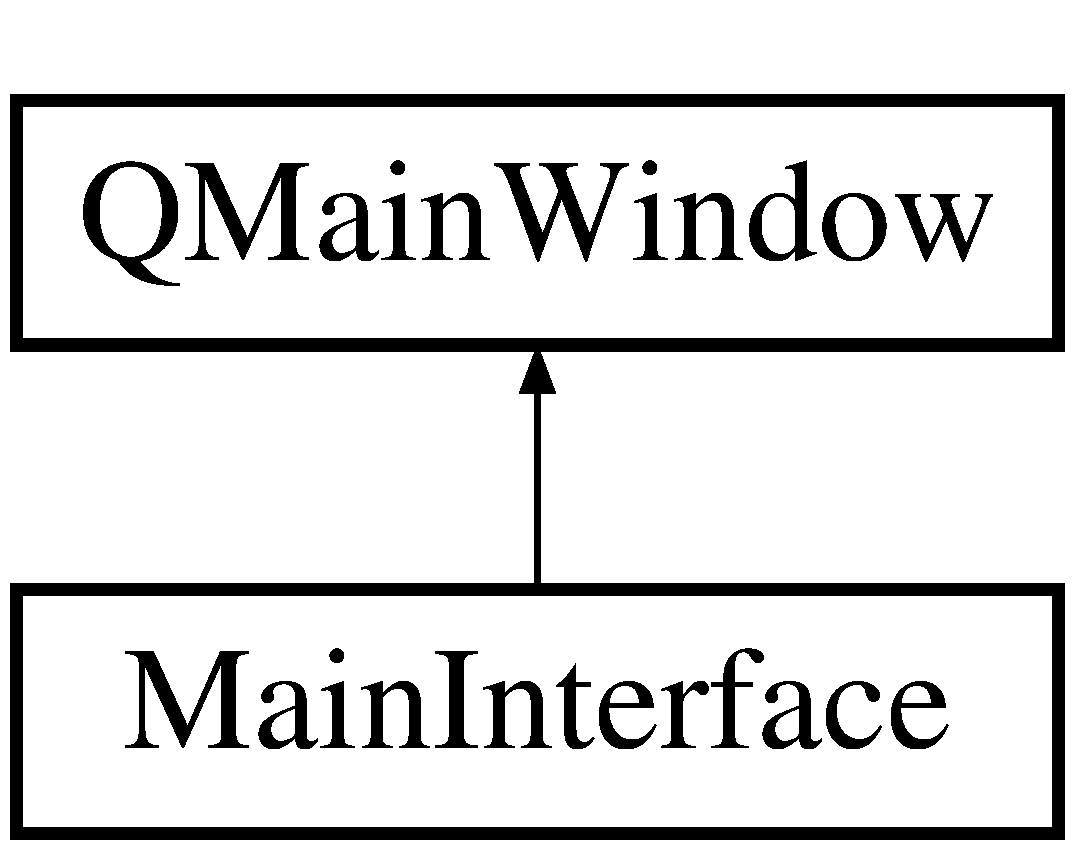
\includegraphics[height=2.000000cm]{class_main_interface}
\end{center}
\end{figure}
\subsection*{Signals}
\begin{DoxyCompactItemize}
\item 
\mbox{\Hypertarget{class_main_interface_aafb8558985bae8b8bc0d58dd0161cb02}\label{class_main_interface_aafb8558985bae8b8bc0d58dd0161cb02}} 
void {\bfseries Point\+Input} ()
\end{DoxyCompactItemize}
\subsection*{Public Member Functions}
\begin{DoxyCompactItemize}
\item 
\mbox{\Hypertarget{class_main_interface_a50ec59f9dc5489bbb18baae382dbc7ad}\label{class_main_interface_a50ec59f9dc5489bbb18baae382dbc7ad}} 
{\bfseries Main\+Interface} (Q\+Widget $\ast$parent=0)
\item 
\mbox{\Hypertarget{class_main_interface_aa5a995b2c60c8c0db5b20a7ff86967d1}\label{class_main_interface_aa5a995b2c60c8c0db5b20a7ff86967d1}} 
void {\bfseries mod\+Current\+Shape} ()
\item 
\mbox{\Hypertarget{class_main_interface_a14e51324b57ebe718257526edd9bde1f}\label{class_main_interface_a14e51324b57ebe718257526edd9bde1f}} 
void {\bfseries new\+Canvas} (int x, int y)
\item 
\mbox{\Hypertarget{class_main_interface_a9e6c88b90697f4c22c4f417387178782}\label{class_main_interface_a9e6c88b90697f4c22c4f417387178782}} 
void {\bfseries load\+Canvas} (Q\+String filename)
\item 
\mbox{\Hypertarget{class_main_interface_a166ca373227ab4e426c7c669b5e7cc09}\label{class_main_interface_a166ca373227ab4e426c7c669b5e7cc09}} 
void {\bfseries change\+Current\+Shape} (Q\+String id\+In)
\item 
\mbox{\Hypertarget{class_main_interface_a7c709f184a028ddfb6b2f61617f76a8b}\label{class_main_interface_a7c709f184a028ddfb6b2f61617f76a8b}} 
void {\bfseries change\+Current\+Shape} (bool is\+Render)
\item 
\mbox{\Hypertarget{class_main_interface_a71ab1f383076fca6850f0dce45ce14a1}\label{class_main_interface_a71ab1f383076fca6850f0dce45ce14a1}} 
void {\bfseries change\+Current\+Shape} (Qt\+::\+Brush\+Style brush\+Style\+In)
\item 
\mbox{\Hypertarget{class_main_interface_af544e40190178d6bfed28264fac5e58d}\label{class_main_interface_af544e40190178d6bfed28264fac5e58d}} 
void {\bfseries change\+Current\+Shape} (Qt\+::\+Global\+Color Color\+In)
\item 
\mbox{\Hypertarget{class_main_interface_af108c59184eb9dab9878f1f43524dd25}\label{class_main_interface_af108c59184eb9dab9878f1f43524dd25}} 
void {\bfseries change\+Current\+Shape} (double penwidth\+IN)
\item 
\mbox{\Hypertarget{class_main_interface_ac39889223f88222ab8b8fa624c07c465}\label{class_main_interface_ac39889223f88222ab8b8fa624c07c465}} 
void {\bfseries change\+Current\+Shape} (Qt\+::\+Pen\+Cap\+Style pen\+Cap\+In)
\item 
\mbox{\Hypertarget{class_main_interface_a15666aefb9526f54640ca363cf2d3b0f}\label{class_main_interface_a15666aefb9526f54640ca363cf2d3b0f}} 
void {\bfseries change\+Current\+Shape} (Qt\+::\+Pen\+Join\+Style pen\+Join\+In)
\item 
\mbox{\Hypertarget{class_main_interface_a10a9313895f905135fdec689d34e7311}\label{class_main_interface_a10a9313895f905135fdec689d34e7311}} 
void {\bfseries change\+Current\+Shape} (Qt\+::\+Pen\+Style pen\+Style\+In)
\item 
Q\+String \hyperlink{class_main_interface_a56a79641ec2a69ce589d01d22a26d41c}{Get\+Shape\+Type} ()
\begin{DoxyCompactList}\small\item\em Get\+Shape\+Type -\/ Returns a string based of the type of shape. \end{DoxyCompactList}\item 
Q\+String \hyperlink{class_main_interface_a4ccc1a9e32a7ad88caceb2acde07c565}{Get\+Shape\+Perimeter\+Area} (bool choice)
\begin{DoxyCompactList}\small\item\em Get\+Shape\+Perimeter\+Area -\/ 0 returns Area, 1 returns Perimeter. \end{DoxyCompactList}\item 
bool \hyperlink{class_main_interface_a5f424dd6f675ae1b55d39c60755cd464}{Has\+Perimeter\+Area} (const \hyperlink{class_shape}{Shape} \&shape)
\begin{DoxyCompactList}\small\item\em Has\+Perimeter\+Area -\/ Returns false if shape does not have Area and Perimeter. \end{DoxyCompactList}\end{DoxyCompactItemize}
\subsection*{Protected Slots}
\begin{DoxyCompactItemize}
\item 
void \hyperlink{class_main_interface_a30d5b73b6b048b5ef9a1095db3a9df23}{change\+Rectdimensions} (double length, double width)
\begin{DoxyCompactList}\small\item\em change\+Rectdimensions -\/ The following methods are situational based off of the type of instance of the shape class there is. i.\+e. rectangle square circle elliser etc. These will probably need to be slots activated when the ui widget is clicked signal \end{DoxyCompactList}\item 
void \hyperlink{class_main_interface_a0331ae438758b87a4658a227d35e39dc}{change\+Squaredimensions} (double length)
\begin{DoxyCompactList}\small\item\em change\+Squaredimensions -\/ example. You use the dynamic casting to in the boolean statment to check if the current shape is an instance of a square. \end{DoxyCompactList}\item 
\mbox{\Hypertarget{class_main_interface_ab9802c99985d57469a9124ae925af8e5}\label{class_main_interface_ab9802c99985d57469a9124ae925af8e5}} 
void {\bfseries change\+Circle\+Radius} (double radius\+In)
\item 
\mbox{\Hypertarget{class_main_interface_af4007d63c3726dce8e968f7d6472fecf}\label{class_main_interface_af4007d63c3726dce8e968f7d6472fecf}} 
void {\bfseries change\+Ellipse\+Axis} (double x\+Rin, double y\+Rin)
\end{DoxyCompactItemize}


\subsection{Detailed Description}
The \hyperlink{class_main_interface}{Main\+Interface} class hold all of the shape classes, handles the changing of shapes via public methods; changing all of the pen and brush styles as well as method that returns the area/perimeter of said shapes. 

\subsection{Member Function Documentation}
\mbox{\Hypertarget{class_main_interface_a30d5b73b6b048b5ef9a1095db3a9df23}\label{class_main_interface_a30d5b73b6b048b5ef9a1095db3a9df23}} 
\index{Main\+Interface@{Main\+Interface}!change\+Rectdimensions@{change\+Rectdimensions}}
\index{change\+Rectdimensions@{change\+Rectdimensions}!Main\+Interface@{Main\+Interface}}
\subsubsection{\texorpdfstring{change\+Rectdimensions}{changeRectdimensions}}
{\footnotesize\ttfamily void Main\+Interface\+::change\+Rectdimensions (\begin{DoxyParamCaption}\item[{double}]{length,  }\item[{double}]{width }\end{DoxyParamCaption})\hspace{0.3cm}{\ttfamily [inline]}, {\ttfamily [protected]}, {\ttfamily [slot]}}



change\+Rectdimensions -\/ The following methods are situational based off of the type of instance of the shape class there is. i.\+e. rectangle square circle elliser etc. These will probably need to be slots activated when the ui widget is clicked signal 


\begin{DoxyParams}{Parameters}
{\em length} & \\
\hline
{\em width} & \\
\hline
\end{DoxyParams}
\mbox{\Hypertarget{class_main_interface_a0331ae438758b87a4658a227d35e39dc}\label{class_main_interface_a0331ae438758b87a4658a227d35e39dc}} 
\index{Main\+Interface@{Main\+Interface}!change\+Squaredimensions@{change\+Squaredimensions}}
\index{change\+Squaredimensions@{change\+Squaredimensions}!Main\+Interface@{Main\+Interface}}
\subsubsection{\texorpdfstring{change\+Squaredimensions}{changeSquaredimensions}}
{\footnotesize\ttfamily void Main\+Interface\+::change\+Squaredimensions (\begin{DoxyParamCaption}\item[{double}]{length }\end{DoxyParamCaption})\hspace{0.3cm}{\ttfamily [inline]}, {\ttfamily [protected]}, {\ttfamily [slot]}}



change\+Squaredimensions -\/ example. You use the dynamic casting to in the boolean statment to check if the current shape is an instance of a square. 


\begin{DoxyParams}{Parameters}
{\em length} & \\
\hline
\end{DoxyParams}
\mbox{\Hypertarget{class_main_interface_a4ccc1a9e32a7ad88caceb2acde07c565}\label{class_main_interface_a4ccc1a9e32a7ad88caceb2acde07c565}} 
\index{Main\+Interface@{Main\+Interface}!Get\+Shape\+Perimeter\+Area@{Get\+Shape\+Perimeter\+Area}}
\index{Get\+Shape\+Perimeter\+Area@{Get\+Shape\+Perimeter\+Area}!Main\+Interface@{Main\+Interface}}
\subsubsection{\texorpdfstring{Get\+Shape\+Perimeter\+Area()}{GetShapePerimeterArea()}}
{\footnotesize\ttfamily Q\+String Main\+Interface\+::\+Get\+Shape\+Perimeter\+Area (\begin{DoxyParamCaption}\item[{bool}]{choice }\end{DoxyParamCaption})}



Get\+Shape\+Perimeter\+Area -\/ 0 returns Area, 1 returns Perimeter. 


\begin{DoxyParams}{Parameters}
{\em choice} & \\
\hline
\end{DoxyParams}
\begin{DoxyReturn}{Returns}

\end{DoxyReturn}
\mbox{\Hypertarget{class_main_interface_a56a79641ec2a69ce589d01d22a26d41c}\label{class_main_interface_a56a79641ec2a69ce589d01d22a26d41c}} 
\index{Main\+Interface@{Main\+Interface}!Get\+Shape\+Type@{Get\+Shape\+Type}}
\index{Get\+Shape\+Type@{Get\+Shape\+Type}!Main\+Interface@{Main\+Interface}}
\subsubsection{\texorpdfstring{Get\+Shape\+Type()}{GetShapeType()}}
{\footnotesize\ttfamily Q\+String Main\+Interface\+::\+Get\+Shape\+Type (\begin{DoxyParamCaption}{ }\end{DoxyParamCaption})}



Get\+Shape\+Type -\/ Returns a string based of the type of shape. 

\begin{DoxyReturn}{Returns}

\end{DoxyReturn}
\mbox{\Hypertarget{class_main_interface_a5f424dd6f675ae1b55d39c60755cd464}\label{class_main_interface_a5f424dd6f675ae1b55d39c60755cd464}} 
\index{Main\+Interface@{Main\+Interface}!Has\+Perimeter\+Area@{Has\+Perimeter\+Area}}
\index{Has\+Perimeter\+Area@{Has\+Perimeter\+Area}!Main\+Interface@{Main\+Interface}}
\subsubsection{\texorpdfstring{Has\+Perimeter\+Area()}{HasPerimeterArea()}}
{\footnotesize\ttfamily bool Main\+Interface\+::\+Has\+Perimeter\+Area (\begin{DoxyParamCaption}\item[{const \hyperlink{class_shape}{Shape} \&}]{shape }\end{DoxyParamCaption})}



Has\+Perimeter\+Area -\/ Returns false if shape does not have Area and Perimeter. 


\begin{DoxyParams}{Parameters}
{\em shape} & \\
\hline
\end{DoxyParams}
\begin{DoxyReturn}{Returns}

\end{DoxyReturn}


The documentation for this class was generated from the following files\+:\begin{DoxyCompactItemize}
\item 
maininterface.\+h\item 
maininterface.\+cpp\end{DoxyCompactItemize}

\hypertarget{class_ui_1_1_main_interface}{}\section{Ui\+:\+:Main\+Interface Class Reference}
\label{class_ui_1_1_main_interface}\index{Ui\+::\+Main\+Interface@{Ui\+::\+Main\+Interface}}
Inheritance diagram for Ui\+:\+:Main\+Interface\+:\begin{figure}[H]
\begin{center}
\leavevmode
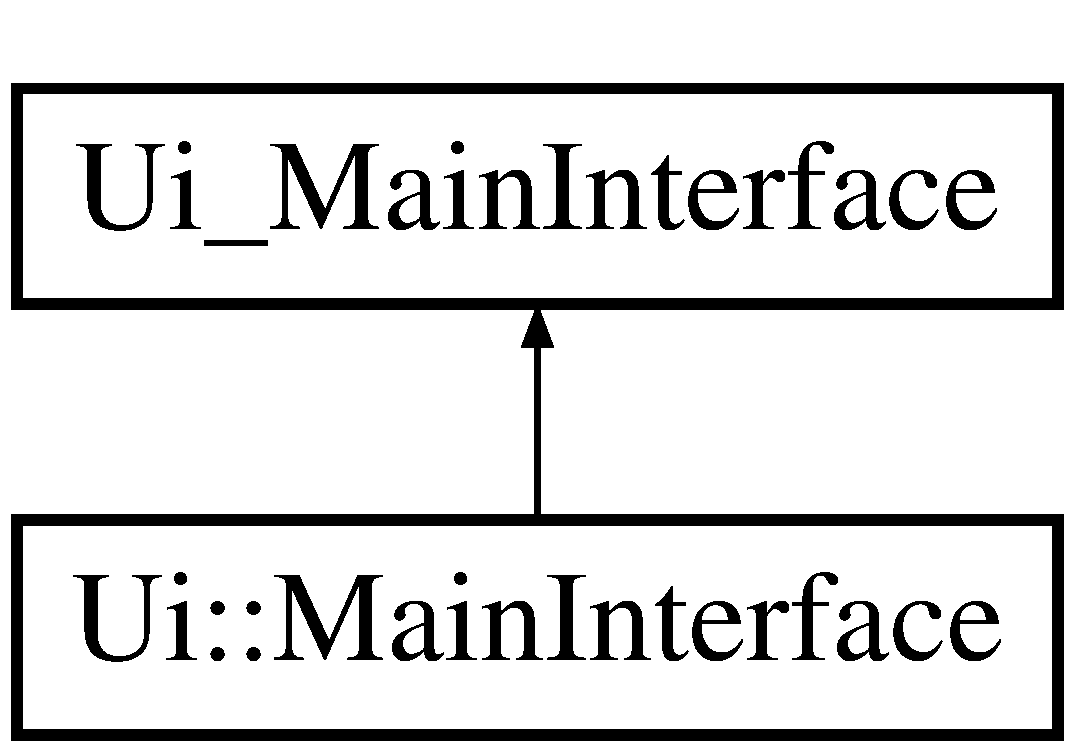
\includegraphics[height=2.000000cm]{class_ui_1_1_main_interface}
\end{center}
\end{figure}
\subsection*{Additional Inherited Members}


The documentation for this class was generated from the following file\+:\begin{DoxyCompactItemize}
\item 
ui\+\_\+maininterface.\+h\end{DoxyCompactItemize}

\hypertarget{class_maintenance_notes}{}\section{Maintenance\+Notes Class Reference}
\label{class_maintenance_notes}\index{Maintenance\+Notes@{Maintenance\+Notes}}
Inheritance diagram for Maintenance\+Notes\+:\begin{figure}[H]
\begin{center}
\leavevmode
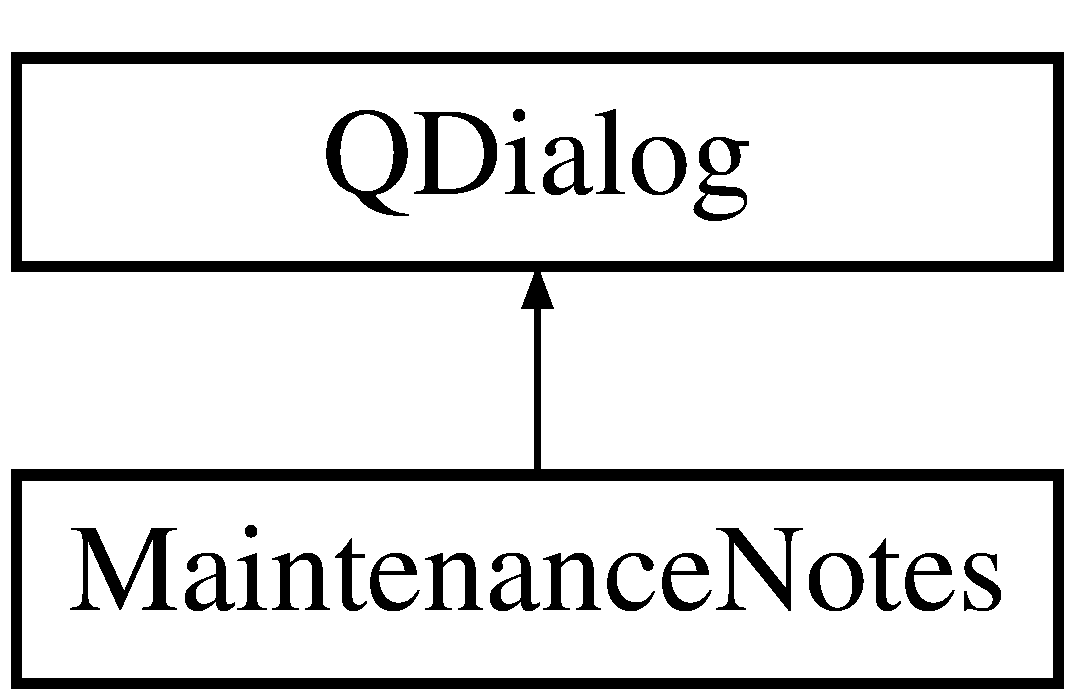
\includegraphics[height=2.000000cm]{class_maintenance_notes}
\end{center}
\end{figure}
\subsection*{Public Member Functions}
\begin{DoxyCompactItemize}
\item 
\mbox{\Hypertarget{class_maintenance_notes_a2292145a9e3a33029b26059b11201ea1}\label{class_maintenance_notes_a2292145a9e3a33029b26059b11201ea1}} 
{\bfseries Maintenance\+Notes} (Q\+Widget $\ast$parent=0)
\end{DoxyCompactItemize}


The documentation for this class was generated from the following files\+:\begin{DoxyCompactItemize}
\item 
maintenancenotes.\+h\item 
maintenancenotes.\+cpp\end{DoxyCompactItemize}

\hypertarget{class_ui_1_1_maintenance_notes}{}\section{Ui\+:\+:Maintenance\+Notes Class Reference}
\label{class_ui_1_1_maintenance_notes}\index{Ui\+::\+Maintenance\+Notes@{Ui\+::\+Maintenance\+Notes}}
Inheritance diagram for Ui\+:\+:Maintenance\+Notes\+:\begin{figure}[H]
\begin{center}
\leavevmode
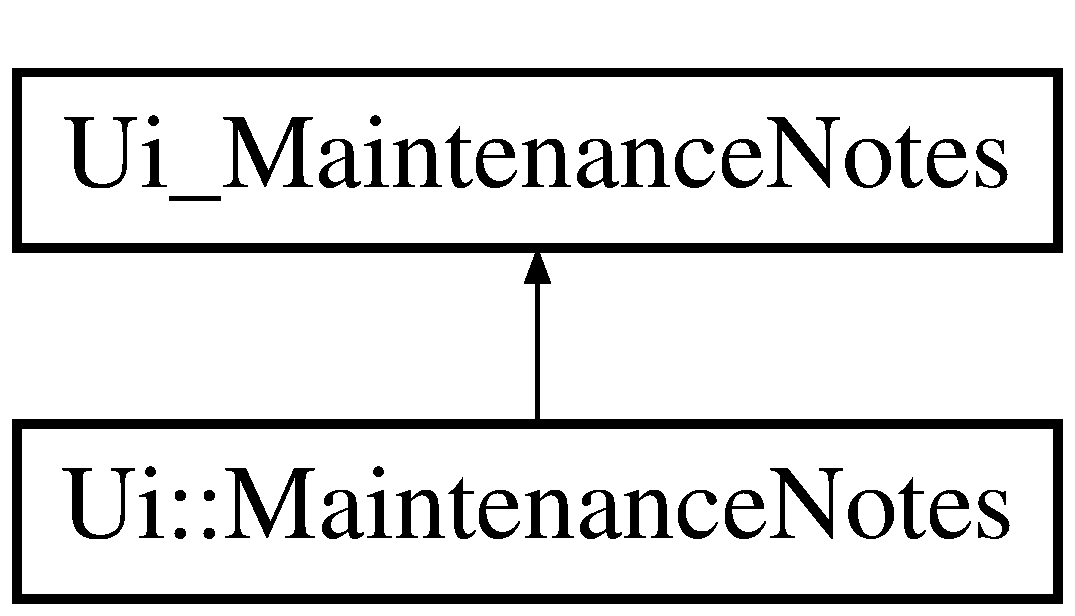
\includegraphics[height=2.000000cm]{class_ui_1_1_maintenance_notes}
\end{center}
\end{figure}
\subsection*{Additional Inherited Members}


The documentation for this class was generated from the following file\+:\begin{DoxyCompactItemize}
\item 
ui\+\_\+maintenancenotes.\+h\end{DoxyCompactItemize}

\hypertarget{classnewnew}{}\section{newnew Class Reference}
\label{classnewnew}\index{newnew@{newnew}}


The newnew class -\/ this is the new login window it handles creating new users as well as checking already exsisting users via the user\+Object object containg a vector of all the exsisting users.  




{\ttfamily \#include $<$newnew.\+h$>$}

Inheritance diagram for newnew\+:\begin{figure}[H]
\begin{center}
\leavevmode
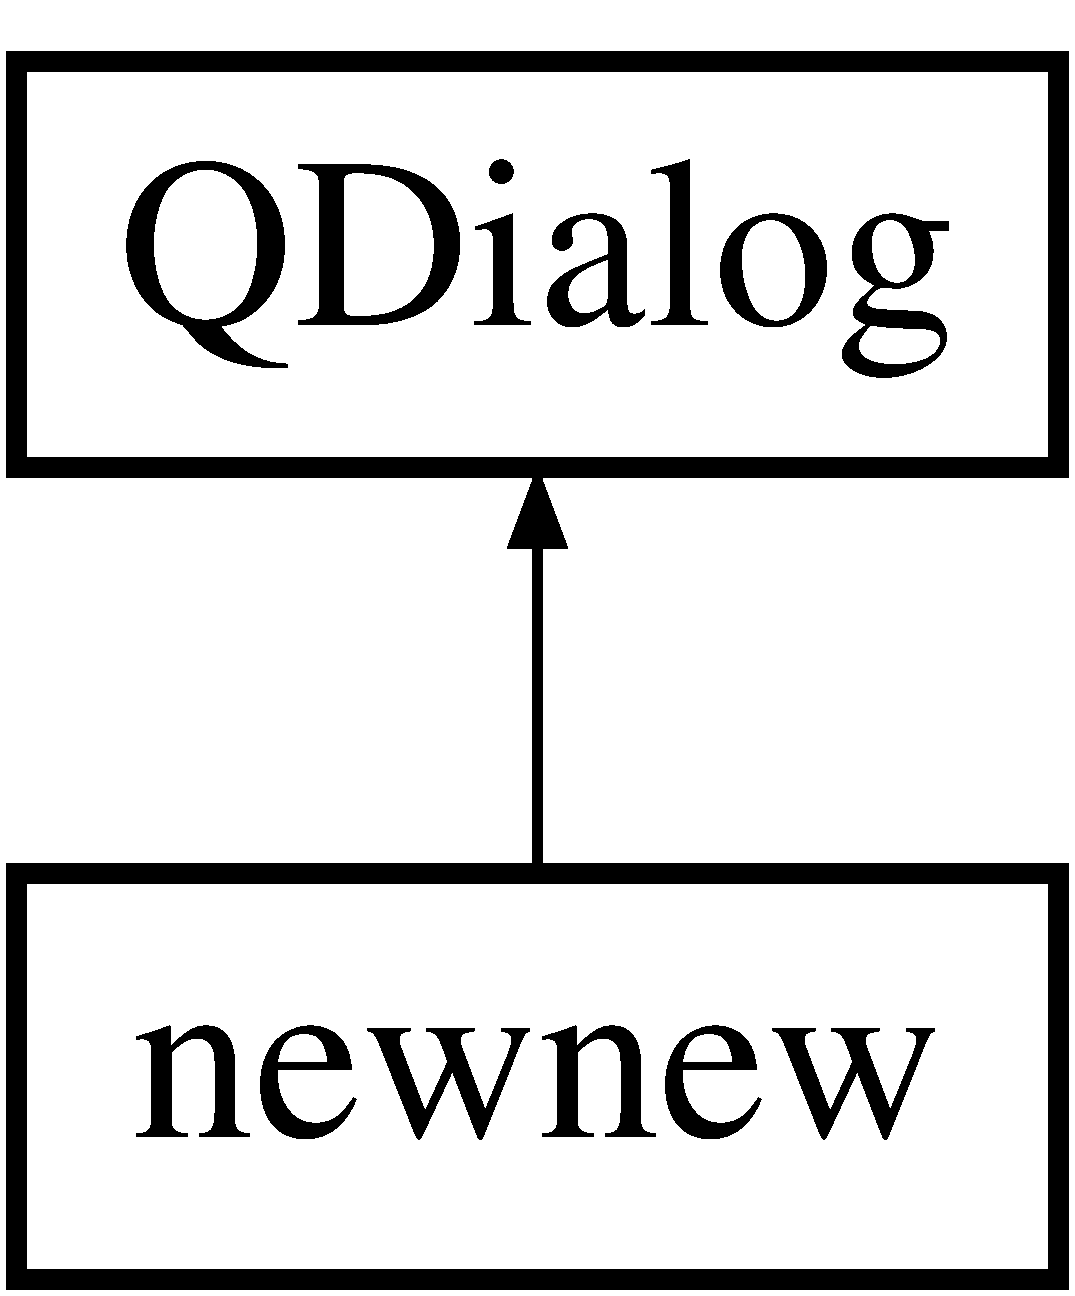
\includegraphics[height=2.000000cm]{classnewnew}
\end{center}
\end{figure}
\subsection*{Public Member Functions}
\begin{DoxyCompactItemize}
\item 
\mbox{\Hypertarget{classnewnew_a2db5641b6b25b8e80f869479459ba06f}\label{classnewnew_a2db5641b6b25b8e80f869479459ba06f}} 
{\bfseries newnew} (Q\+Widget $\ast$parent=0)
\item 
void \hyperlink{classnewnew_a03d2e950f73da3c67048a0f736b90c3f}{start\+Movie} (Q\+Movie \&gif)
\begin{DoxyCompactList}\small\item\em start\+Movie -\/ function call to play the gif animation \end{DoxyCompactList}\end{DoxyCompactItemize}


\subsection{Detailed Description}
The newnew class -\/ this is the new login window it handles creating new users as well as checking already exsisting users via the user\+Object object containg a vector of all the exsisting users. 

\subsection{Member Function Documentation}
\mbox{\Hypertarget{classnewnew_a03d2e950f73da3c67048a0f736b90c3f}\label{classnewnew_a03d2e950f73da3c67048a0f736b90c3f}} 
\index{newnew@{newnew}!start\+Movie@{start\+Movie}}
\index{start\+Movie@{start\+Movie}!newnew@{newnew}}
\subsubsection{\texorpdfstring{start\+Movie()}{startMovie()}}
{\footnotesize\ttfamily void newnew\+::start\+Movie (\begin{DoxyParamCaption}\item[{Q\+Movie \&}]{gif }\end{DoxyParamCaption})}



start\+Movie -\/ function call to play the gif animation 


\begin{DoxyParams}{Parameters}
{\em gif} & \\
\hline
\end{DoxyParams}


The documentation for this class was generated from the following files\+:\begin{DoxyCompactItemize}
\item 
newnew.\+h\item 
newnew.\+cpp\end{DoxyCompactItemize}

\hypertarget{class_ui_1_1newnew}{}\section{Ui\+:\+:newnew Class Reference}
\label{class_ui_1_1newnew}\index{Ui\+::newnew@{Ui\+::newnew}}
Inheritance diagram for Ui\+:\+:newnew\+:\begin{figure}[H]
\begin{center}
\leavevmode
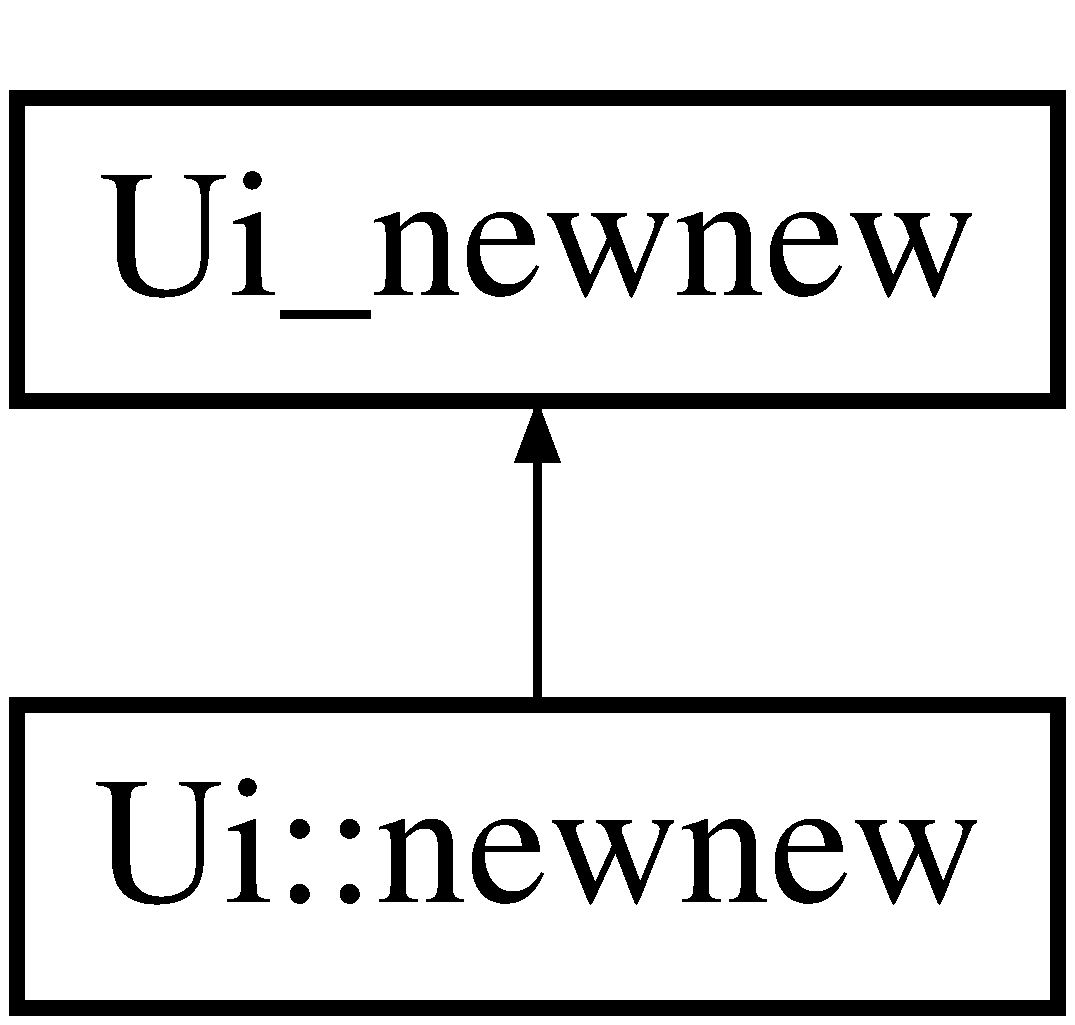
\includegraphics[height=2.000000cm]{class_ui_1_1newnew}
\end{center}
\end{figure}
\subsection*{Additional Inherited Members}


The documentation for this class was generated from the following file\+:\begin{DoxyCompactItemize}
\item 
ui\+\_\+newnew.\+h\end{DoxyCompactItemize}

\hypertarget{class_polygon}{}\section{Polygon Class Reference}
\label{class_polygon}\index{Polygon@{Polygon}}


The \hyperlink{class_polygon}{Polygon} class -\/ derives form the Polyline class set to make polygon shapes.  




{\ttfamily \#include $<$Poly\+Gon.\+h$>$}

Inheritance diagram for Polygon\+:\begin{figure}[H]
\begin{center}
\leavevmode
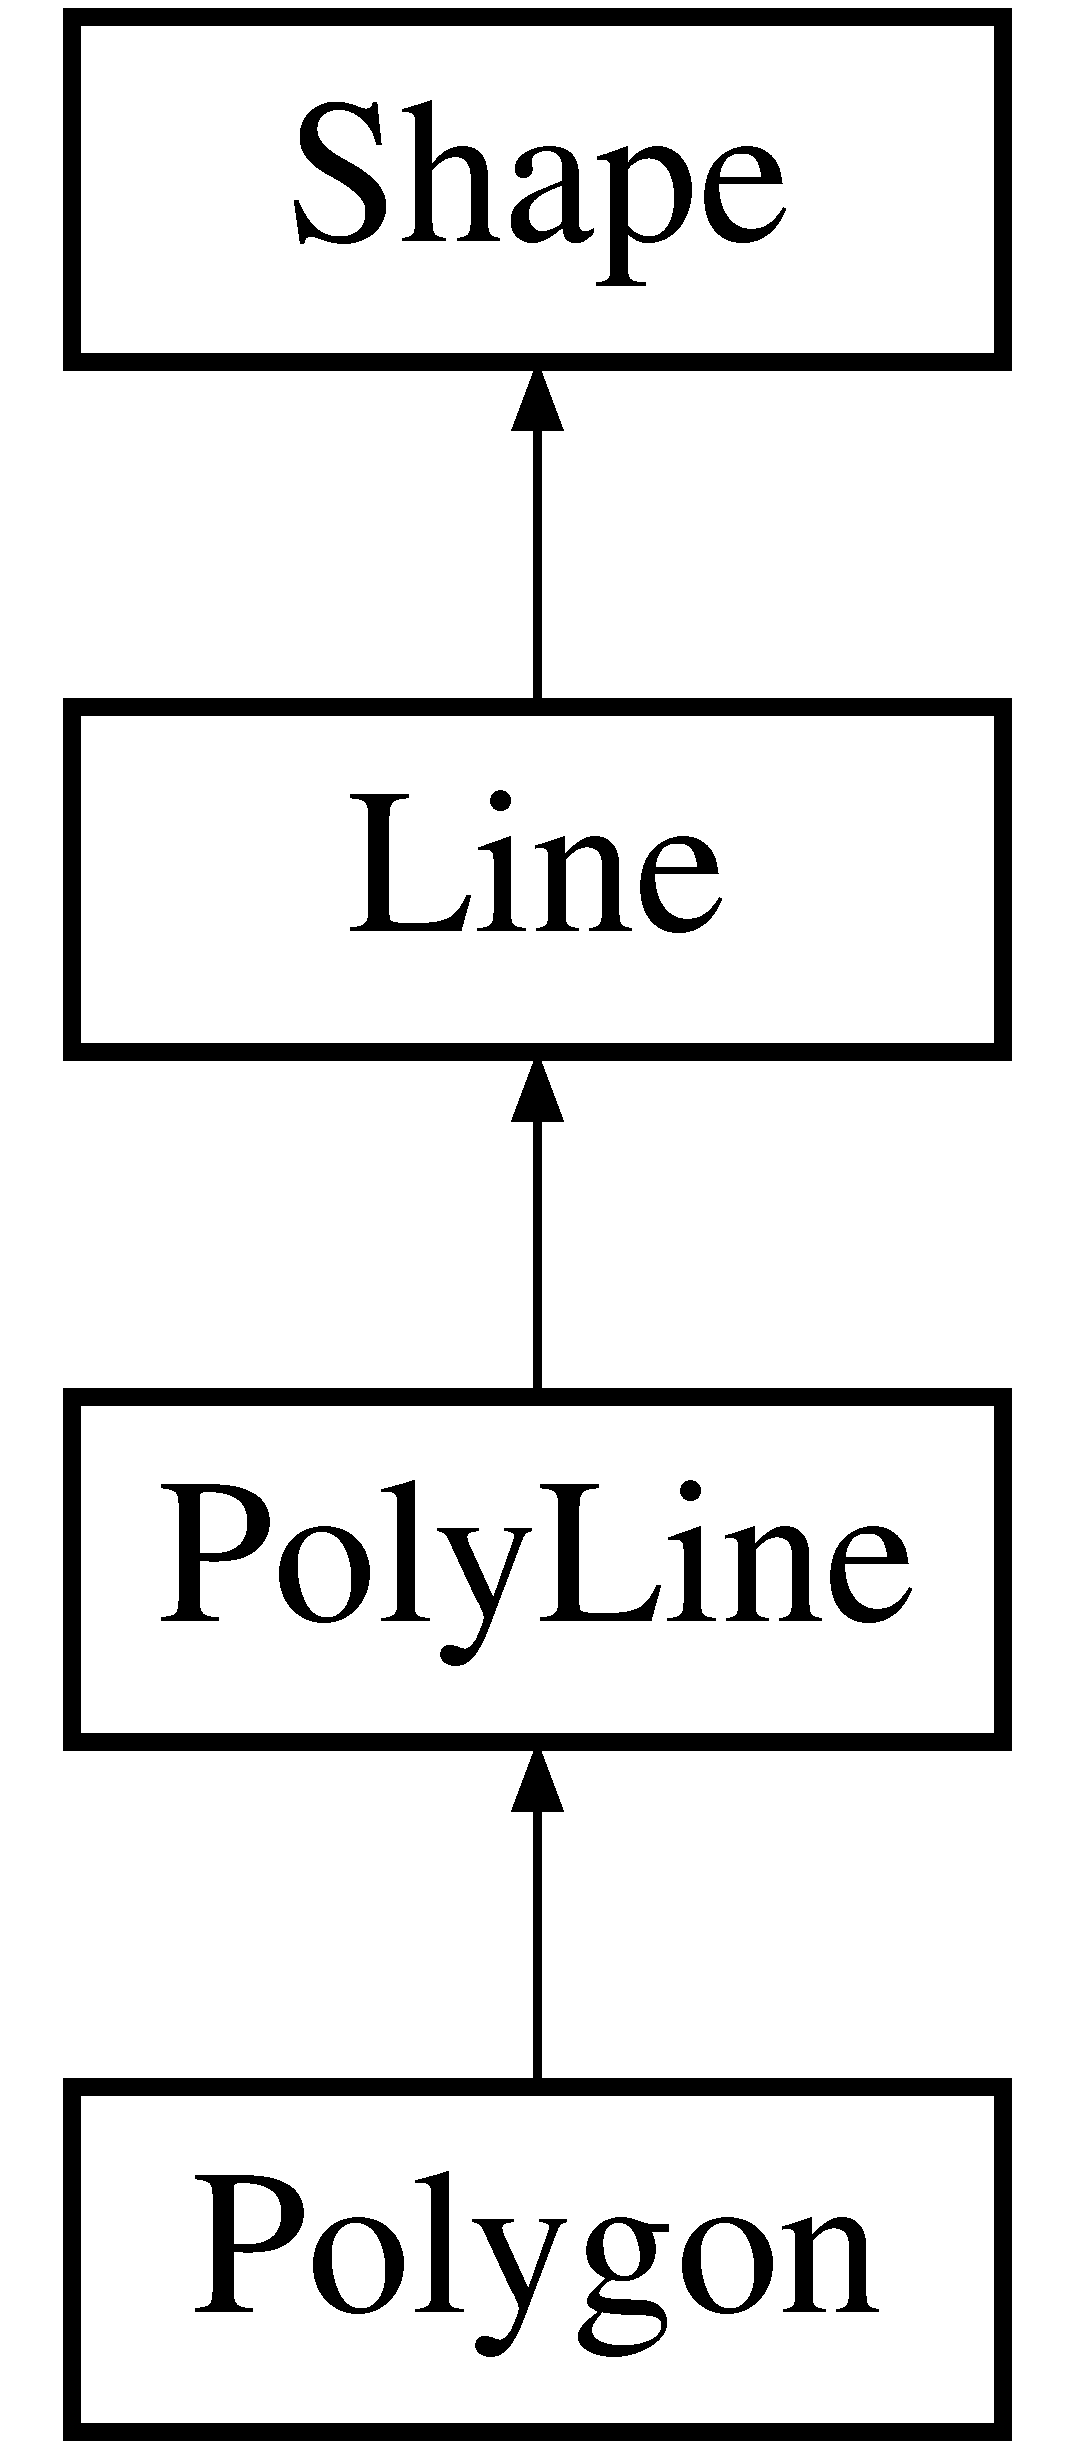
\includegraphics[height=4.000000cm]{class_polygon}
\end{center}
\end{figure}
\subsection*{Public Member Functions}
\begin{DoxyCompactItemize}
\item 
\mbox{\Hypertarget{class_polygon_a500d5ae5db7a63abe140f6f050f5d626}\label{class_polygon_a500d5ae5db7a63abe140f6f050f5d626}} 
{\bfseries Polygon} (Q\+String id\+In, Qt\+::\+Brush\+Style brush\+Style\+In, Qt\+::\+Global\+Color brush\+Color\+In, double pen\+Width\+In, Qt\+::\+Global\+Color pen\+Color\+In, Qt\+::\+Pen\+Cap\+Style pen\+Cap\+In, Qt\+::\+Pen\+Join\+Style pen\+Join\+In, Qt\+::\+Pen\+Style pen\+Style\+In)
\item 
virtual void \hyperlink{class_polygon_ad57f4b375c6858bfe34c095bfeb38d5a}{push\+\_\+\+Back\+\_\+point} (Q\+Point xy)
\begin{DoxyCompactList}\small\item\em push\+\_\+\+Back\+\_\+point -\/ just like class\+::line we use the pushback virtual functions to obtain the mouse input coordinates on where to create the polyline \end{DoxyCompactList}\item 
\mbox{\Hypertarget{class_polygon_ac61aa8a55c4f57c8242af92e0f65aa0a}\label{class_polygon_ac61aa8a55c4f57c8242af92e0f65aa0a}} 
virtual void {\bfseries push\+\_\+\+Back\+\_\+point} (int x, int y)
\item 
virtual void \hyperlink{class_polygon_a9271921d96331c203efcdb50e0ebd64c}{Draw} (\hyperlink{class_canvas}{Canvas} $\ast$draw\+Area)
\begin{DoxyCompactList}\small\item\em Draw. \end{DoxyCompactList}\item 
virtual bool \hyperlink{class_polygon_ab17f2f8ae9489fba4030fbb4a99e7ea6}{is\+\_\+\+Left\+\_\+\+Clicked} (Q\+Point e)
\begin{DoxyCompactList}\small\item\em is\+\_\+\+Left\+\_\+\+Clicked -\/ mouse input \end{DoxyCompactList}\end{DoxyCompactItemize}
\subsection*{Additional Inherited Members}


\subsection{Detailed Description}
The \hyperlink{class_polygon}{Polygon} class -\/ derives form the Polyline class set to make polygon shapes. 

\subsection{Member Function Documentation}
\mbox{\Hypertarget{class_polygon_a9271921d96331c203efcdb50e0ebd64c}\label{class_polygon_a9271921d96331c203efcdb50e0ebd64c}} 
\index{Polygon@{Polygon}!Draw@{Draw}}
\index{Draw@{Draw}!Polygon@{Polygon}}
\subsubsection{\texorpdfstring{Draw()}{Draw()}}
{\footnotesize\ttfamily void Polygon\+::\+Draw (\begin{DoxyParamCaption}\item[{\hyperlink{class_canvas}{Canvas} $\ast$}]{draw\+Area }\end{DoxyParamCaption})\hspace{0.3cm}{\ttfamily [virtual]}}



Draw. 


\begin{DoxyParams}{Parameters}
{\em draw\+Area} & \\
\hline
\end{DoxyParams}


Reimplemented from \hyperlink{class_poly_line_ac42ca364849f33b899a929bf57163730}{Poly\+Line}.

\mbox{\Hypertarget{class_polygon_ab17f2f8ae9489fba4030fbb4a99e7ea6}\label{class_polygon_ab17f2f8ae9489fba4030fbb4a99e7ea6}} 
\index{Polygon@{Polygon}!is\+\_\+\+Left\+\_\+\+Clicked@{is\+\_\+\+Left\+\_\+\+Clicked}}
\index{is\+\_\+\+Left\+\_\+\+Clicked@{is\+\_\+\+Left\+\_\+\+Clicked}!Polygon@{Polygon}}
\subsubsection{\texorpdfstring{is\+\_\+\+Left\+\_\+\+Clicked()}{is\_Left\_Clicked()}}
{\footnotesize\ttfamily bool Polygon\+::is\+\_\+\+Left\+\_\+\+Clicked (\begin{DoxyParamCaption}\item[{Q\+Point}]{e }\end{DoxyParamCaption})\hspace{0.3cm}{\ttfamily [virtual]}}



is\+\_\+\+Left\+\_\+\+Clicked -\/ mouse input 


\begin{DoxyParams}{Parameters}
{\em e} & \\
\hline
\end{DoxyParams}
\begin{DoxyReturn}{Returns}

\end{DoxyReturn}


Reimplemented from \hyperlink{class_poly_line_a349f5b14d3ab568ae6776a3d5fd6f956}{Poly\+Line}.

\mbox{\Hypertarget{class_polygon_ad57f4b375c6858bfe34c095bfeb38d5a}\label{class_polygon_ad57f4b375c6858bfe34c095bfeb38d5a}} 
\index{Polygon@{Polygon}!push\+\_\+\+Back\+\_\+point@{push\+\_\+\+Back\+\_\+point}}
\index{push\+\_\+\+Back\+\_\+point@{push\+\_\+\+Back\+\_\+point}!Polygon@{Polygon}}
\subsubsection{\texorpdfstring{push\+\_\+\+Back\+\_\+point()}{push\_Back\_point()}}
{\footnotesize\ttfamily void Polygon\+::push\+\_\+\+Back\+\_\+point (\begin{DoxyParamCaption}\item[{Q\+Point}]{xy }\end{DoxyParamCaption})\hspace{0.3cm}{\ttfamily [virtual]}}



push\+\_\+\+Back\+\_\+point -\/ just like class\+::line we use the pushback virtual functions to obtain the mouse input coordinates on where to create the polyline 


\begin{DoxyParams}{Parameters}
{\em xy} & \\
\hline
\end{DoxyParams}


Reimplemented from \hyperlink{class_poly_line_afbc3a0e59abcd27bdb58027796e91c3a}{Poly\+Line}.



The documentation for this class was generated from the following files\+:\begin{DoxyCompactItemize}
\item 
Poly\+Gon.\+h\item 
Polygon.\+cpp\end{DoxyCompactItemize}

\hypertarget{class_poly_line}{}\section{Poly\+Line Class Reference}
\label{class_poly_line}\index{Poly\+Line@{Poly\+Line}}


The \hyperlink{class_poly_line}{Poly\+Line} class -\/ derives from line.  




{\ttfamily \#include $<$Poly\+Line.\+h$>$}

Inheritance diagram for Poly\+Line\+:\begin{figure}[H]
\begin{center}
\leavevmode
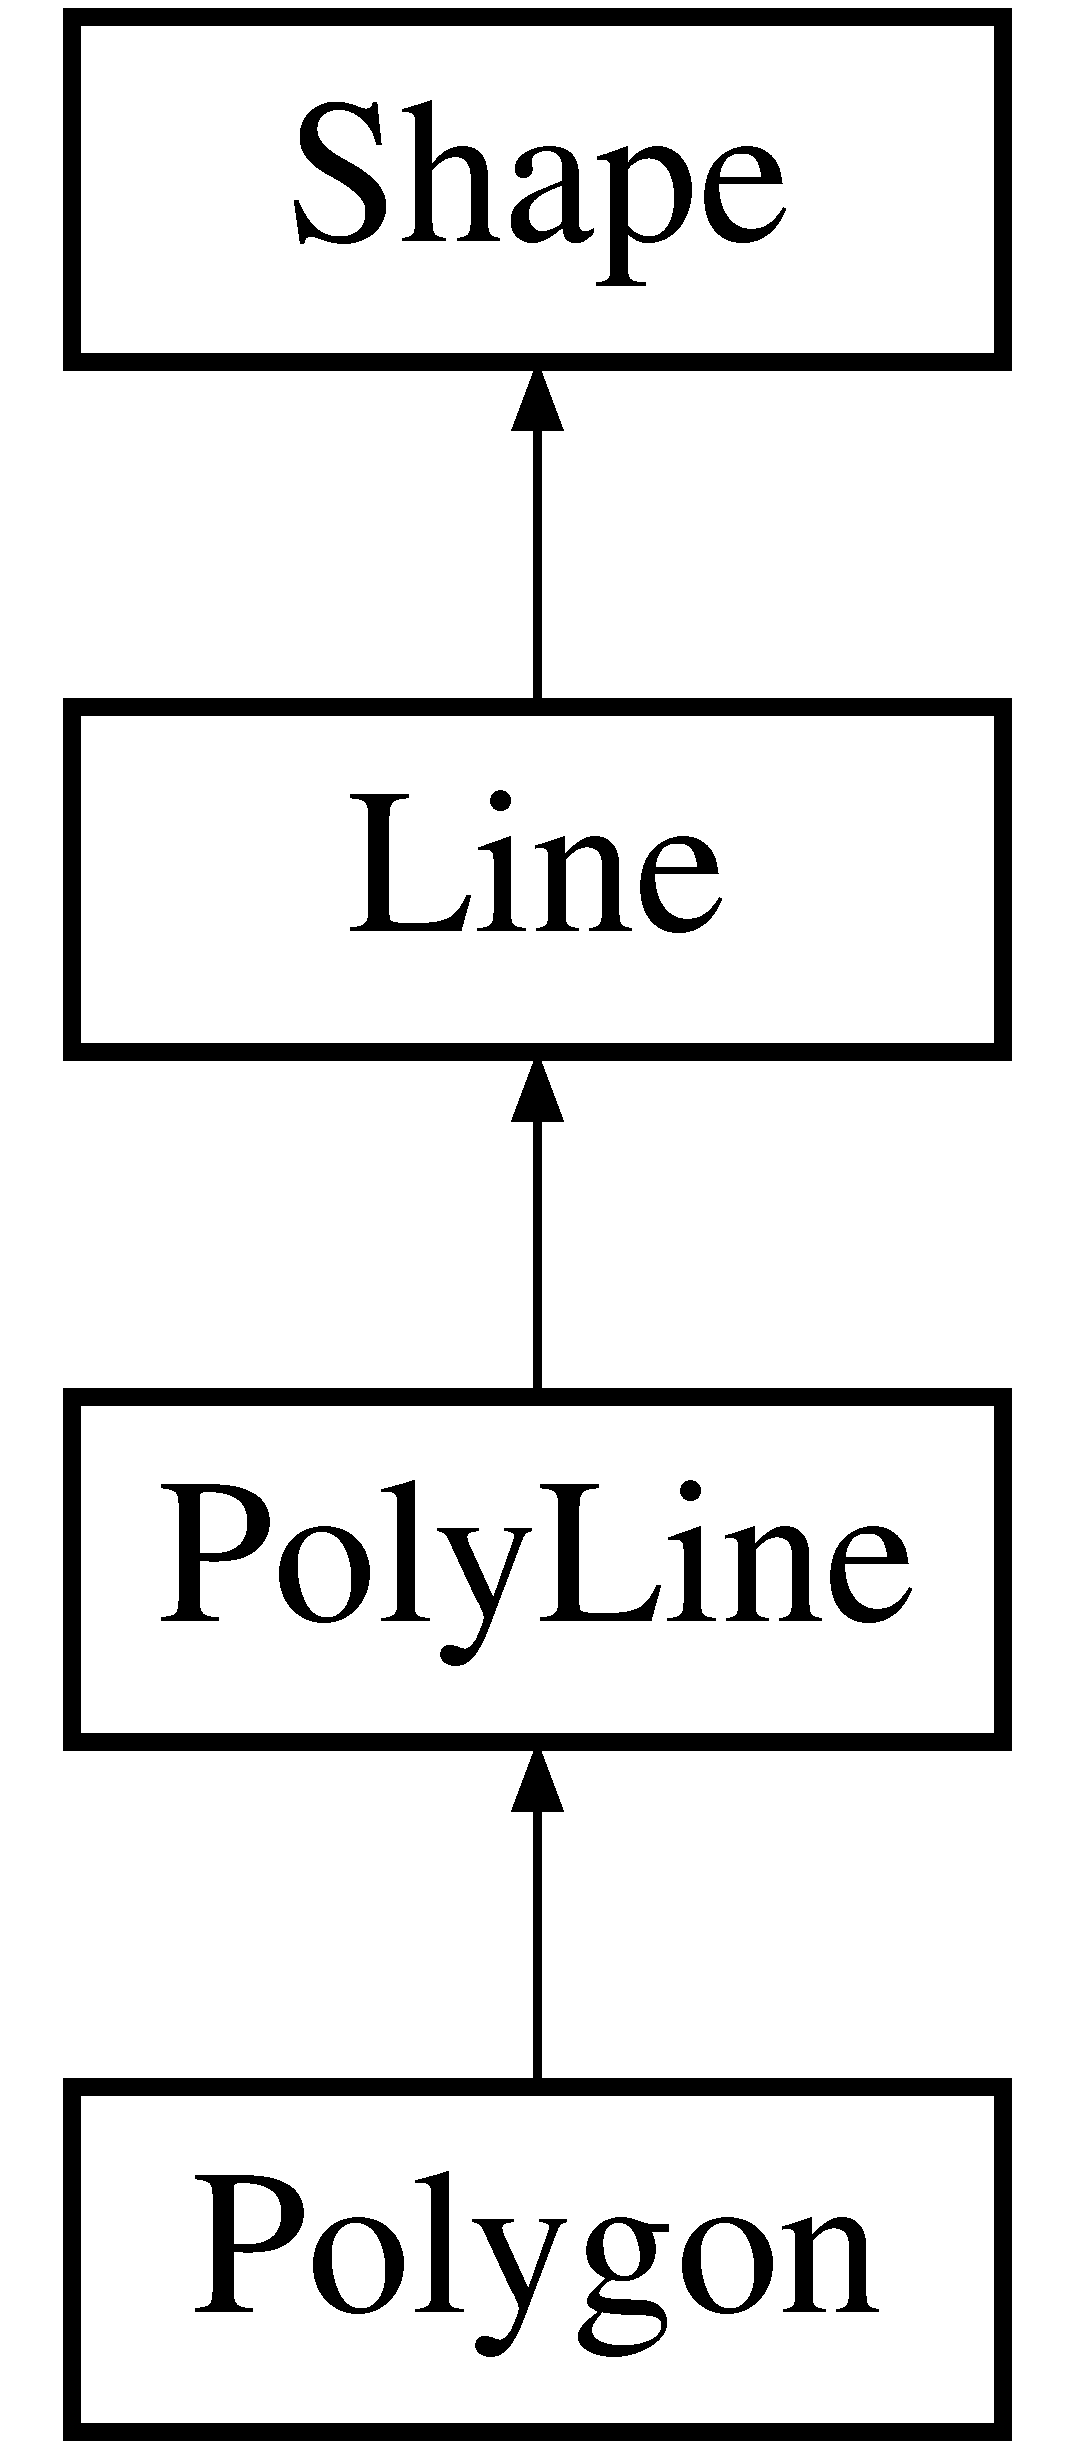
\includegraphics[height=4.000000cm]{class_poly_line}
\end{center}
\end{figure}
\subsection*{Public Member Functions}
\begin{DoxyCompactItemize}
\item 
\mbox{\Hypertarget{class_poly_line_a5f896d603d3f1d495ba4cb647c771a96}\label{class_poly_line_a5f896d603d3f1d495ba4cb647c771a96}} 
{\bfseries Poly\+Line} (Q\+String id\+In, Qt\+::\+Brush\+Style brush\+Style\+In, Qt\+::\+Global\+Color brush\+Color\+In, double pen\+Width\+In, Qt\+::\+Global\+Color pen\+Color\+In, Qt\+::\+Pen\+Cap\+Style pen\+Cap\+In, Qt\+::\+Pen\+Join\+Style pen\+Join\+In, Qt\+::\+Pen\+Style pen\+Style\+In)
\item 
virtual void \hyperlink{class_poly_line_afbc3a0e59abcd27bdb58027796e91c3a}{push\+\_\+\+Back\+\_\+point} (Q\+Point xy)
\begin{DoxyCompactList}\small\item\em push\+\_\+\+Back\+\_\+point -\/ see polygon/line documentation of the functions below \end{DoxyCompactList}\item 
\mbox{\Hypertarget{class_poly_line_a3a2483c862ffa1f31157d7fd510dca6c}\label{class_poly_line_a3a2483c862ffa1f31157d7fd510dca6c}} 
virtual void {\bfseries push\+\_\+\+Back\+\_\+point} (int x, int y)
\item 
\mbox{\Hypertarget{class_poly_line_a73a4db1130cb26bba52e750ae27e7fd8}\label{class_poly_line_a73a4db1130cb26bba52e750ae27e7fd8}} 
virtual void {\bfseries move\+Last\+Point} (Q\+Point e)
\item 
virtual void \hyperlink{class_poly_line_ac42ca364849f33b899a929bf57163730}{Draw} (\hyperlink{class_canvas}{Canvas} $\ast$draw\+Area)
\begin{DoxyCompactList}\small\item\em Draw -\/ draws the shape\+: virtual. \end{DoxyCompactList}\item 
virtual bool \hyperlink{class_poly_line_a349f5b14d3ab568ae6776a3d5fd6f956}{is\+\_\+\+Left\+\_\+\+Clicked} (Q\+Point e)
\begin{DoxyCompactList}\small\item\em is\+\_\+\+Left\+\_\+\+Clicked -\/ mouse input \end{DoxyCompactList}\end{DoxyCompactItemize}
\subsection*{Additional Inherited Members}


\subsection{Detailed Description}
The \hyperlink{class_poly_line}{Poly\+Line} class -\/ derives from line. 

\subsection{Member Function Documentation}
\mbox{\Hypertarget{class_poly_line_ac42ca364849f33b899a929bf57163730}\label{class_poly_line_ac42ca364849f33b899a929bf57163730}} 
\index{Poly\+Line@{Poly\+Line}!Draw@{Draw}}
\index{Draw@{Draw}!Poly\+Line@{Poly\+Line}}
\subsubsection{\texorpdfstring{Draw()}{Draw()}}
{\footnotesize\ttfamily void Poly\+Line\+::\+Draw (\begin{DoxyParamCaption}\item[{\hyperlink{class_canvas}{Canvas} $\ast$}]{paint\+Area }\end{DoxyParamCaption})\hspace{0.3cm}{\ttfamily [virtual]}}



Draw -\/ draws the shape\+: virtual. 


\begin{DoxyParams}{Parameters}
{\em paint\+Area} & \\
\hline
\end{DoxyParams}


Reimplemented from \hyperlink{class_line_ae645f8a7f03439fa3428f81b1ddb4ffc}{Line}.



Reimplemented in \hyperlink{class_polygon_a9271921d96331c203efcdb50e0ebd64c}{Polygon}.

\mbox{\Hypertarget{class_poly_line_a349f5b14d3ab568ae6776a3d5fd6f956}\label{class_poly_line_a349f5b14d3ab568ae6776a3d5fd6f956}} 
\index{Poly\+Line@{Poly\+Line}!is\+\_\+\+Left\+\_\+\+Clicked@{is\+\_\+\+Left\+\_\+\+Clicked}}
\index{is\+\_\+\+Left\+\_\+\+Clicked@{is\+\_\+\+Left\+\_\+\+Clicked}!Poly\+Line@{Poly\+Line}}
\subsubsection{\texorpdfstring{is\+\_\+\+Left\+\_\+\+Clicked()}{is\_Left\_Clicked()}}
{\footnotesize\ttfamily bool Poly\+Line\+::is\+\_\+\+Left\+\_\+\+Clicked (\begin{DoxyParamCaption}\item[{Q\+Point}]{e }\end{DoxyParamCaption})\hspace{0.3cm}{\ttfamily [virtual]}}



is\+\_\+\+Left\+\_\+\+Clicked -\/ mouse input 


\begin{DoxyParams}{Parameters}
{\em e} & \\
\hline
\end{DoxyParams}
\begin{DoxyReturn}{Returns}

\end{DoxyReturn}


Reimplemented from \hyperlink{class_line_a79c3891fefd740e6a3cfcdb57a105995}{Line}.



Reimplemented in \hyperlink{class_polygon_ab17f2f8ae9489fba4030fbb4a99e7ea6}{Polygon}.

\mbox{\Hypertarget{class_poly_line_afbc3a0e59abcd27bdb58027796e91c3a}\label{class_poly_line_afbc3a0e59abcd27bdb58027796e91c3a}} 
\index{Poly\+Line@{Poly\+Line}!push\+\_\+\+Back\+\_\+point@{push\+\_\+\+Back\+\_\+point}}
\index{push\+\_\+\+Back\+\_\+point@{push\+\_\+\+Back\+\_\+point}!Poly\+Line@{Poly\+Line}}
\subsubsection{\texorpdfstring{push\+\_\+\+Back\+\_\+point()}{push\_Back\_point()}}
{\footnotesize\ttfamily void Poly\+Line\+::push\+\_\+\+Back\+\_\+point (\begin{DoxyParamCaption}\item[{Q\+Point}]{xy }\end{DoxyParamCaption})\hspace{0.3cm}{\ttfamily [virtual]}}



push\+\_\+\+Back\+\_\+point -\/ see polygon/line documentation of the functions below 


\begin{DoxyParams}{Parameters}
{\em xy} & \\
\hline
\end{DoxyParams}


Reimplemented from \hyperlink{class_line_a01ac38eae66f157868daee1b4764b242}{Line}.



Reimplemented in \hyperlink{class_polygon_ad57f4b375c6858bfe34c095bfeb38d5a}{Polygon}.



The documentation for this class was generated from the following files\+:\begin{DoxyCompactItemize}
\item 
Poly\+Line.\+h\item 
polyline.\+cpp\end{DoxyCompactItemize}

\hypertarget{class_rectangle}{}\section{Rectangle Class Reference}
\label{class_rectangle}\index{Rectangle@{Rectangle}}


The \hyperlink{class_rectangle}{Rectangle} class -\/ derives from abstract base class\+: shape.  




{\ttfamily \#include $<$Rectangle.\+h$>$}

Inheritance diagram for Rectangle\+:\begin{figure}[H]
\begin{center}
\leavevmode
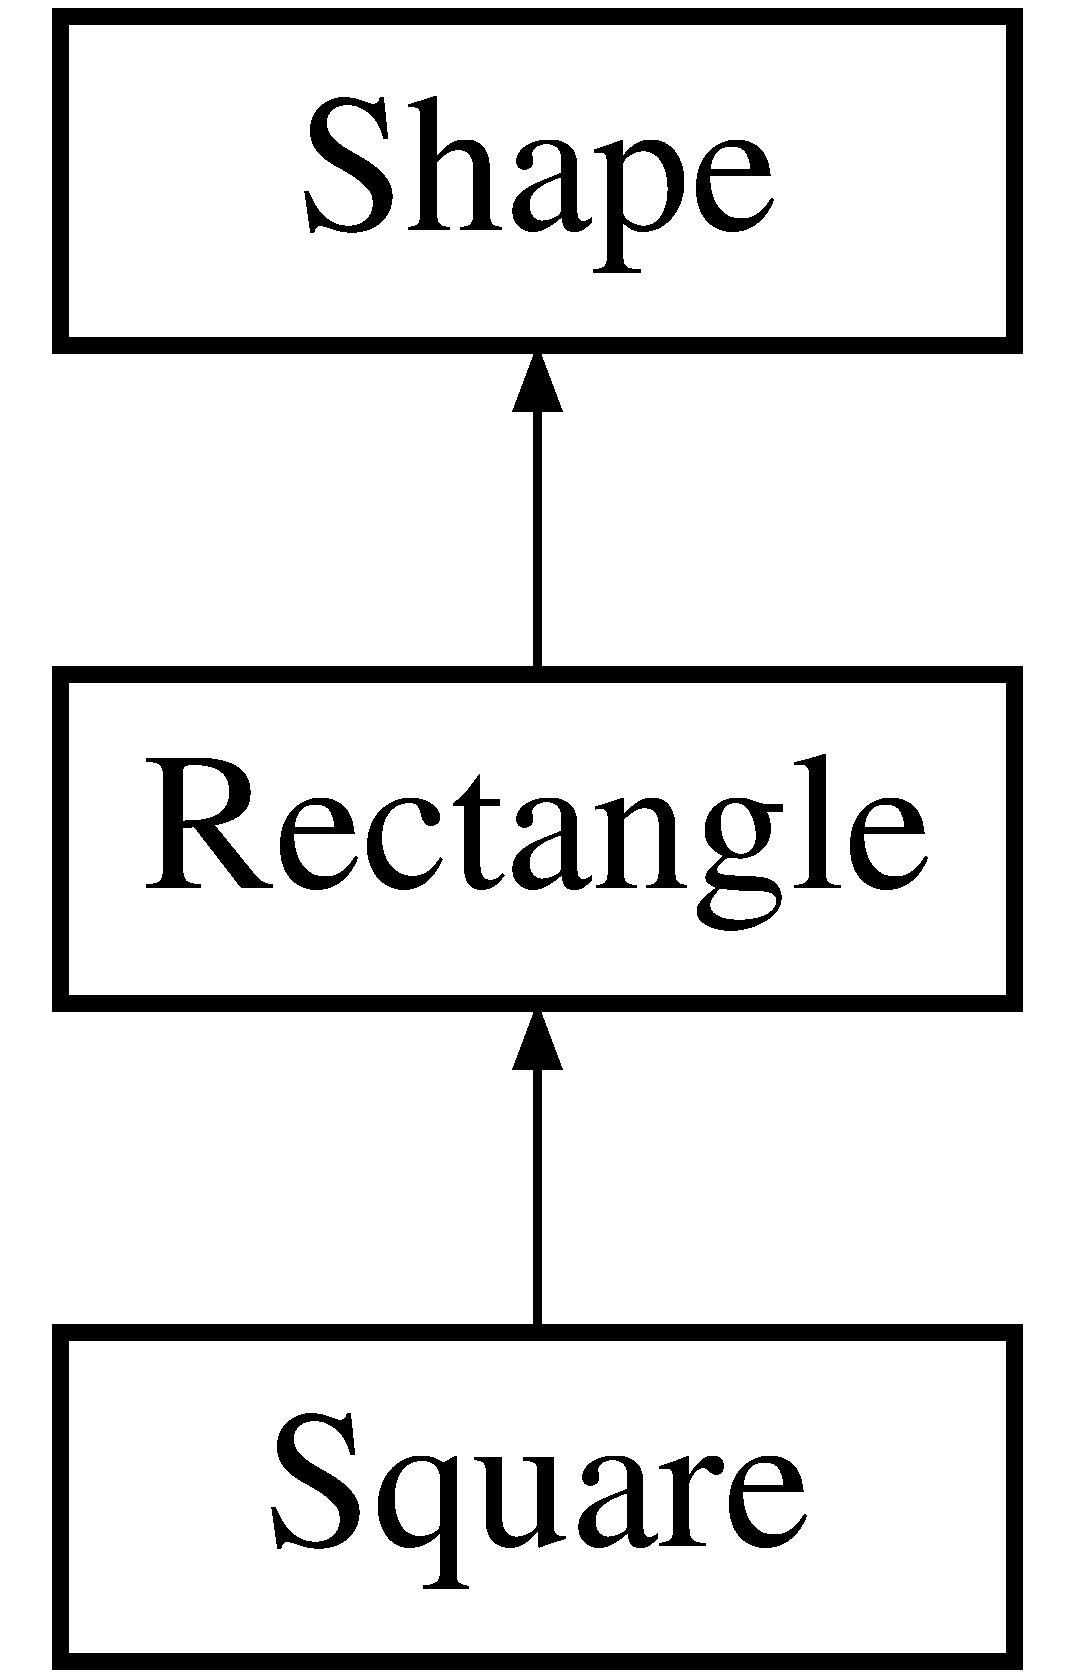
\includegraphics[height=3.000000cm]{class_rectangle}
\end{center}
\end{figure}
\subsection*{Public Member Functions}
\begin{DoxyCompactItemize}
\item 
\mbox{\Hypertarget{class_rectangle_a45ea4c7e76ce39d3a84104302469459c}\label{class_rectangle_a45ea4c7e76ce39d3a84104302469459c}} 
{\bfseries Rectangle} (int x, int y, double w, double l)
\item 
\mbox{\Hypertarget{class_rectangle_ad2c25ea89c4241b8bce1d4f5968986cb}\label{class_rectangle_ad2c25ea89c4241b8bce1d4f5968986cb}} 
{\bfseries Rectangle} (Q\+String id\+In, Qt\+::\+Brush\+Style brush\+Style\+In, Qt\+::\+Global\+Color brush\+Color\+In, double pen\+Width\+In, Qt\+::\+Global\+Color pen\+Color\+In, Qt\+::\+Pen\+Cap\+Style pen\+Cap\+In, Qt\+::\+Pen\+Join\+Style pen\+Join\+In, Qt\+::\+Pen\+Style pen\+Style\+In, double xR, double yR)
\item 
\mbox{\Hypertarget{class_rectangle_a777b92b37ee95a1285bd7dddf8c61a40}\label{class_rectangle_a777b92b37ee95a1285bd7dddf8c61a40}} 
{\bfseries Rectangle} (\hyperlink{class_rectangle}{Rectangle} \&copy)
\item 
\mbox{\Hypertarget{class_rectangle_a3237955de5a7ae91bb0f617bc245c55e}\label{class_rectangle_a3237955de5a7ae91bb0f617bc245c55e}} 
{\bfseries Rectangle} (\hyperlink{class_rectangle}{Rectangle} \&\&copy)
\item 
\mbox{\Hypertarget{class_rectangle_a248979d5af0684e056dcb4715f4b1e1e}\label{class_rectangle_a248979d5af0684e056dcb4715f4b1e1e}} 
void {\bfseries set\+Width\+Length} (double w, double l)
\item 
\mbox{\Hypertarget{class_rectangle_a73685e64359134d26b57886aca27c1e7}\label{class_rectangle_a73685e64359134d26b57886aca27c1e7}} 
void {\bfseries set\+Width} (double w)
\item 
\mbox{\Hypertarget{class_rectangle_a4401ebc484718df223089cb442a2f813}\label{class_rectangle_a4401ebc484718df223089cb442a2f813}} 
void {\bfseries set\+Length} (double l)
\item 
virtual void \hyperlink{class_rectangle_abeeafbc4d44bf241cf655e850f3ce3f3}{move} (Q\+Point xy)
\begin{DoxyCompactList}\small\item\em move -\/ handles moving the shape and recieves in mouse input \end{DoxyCompactList}\item 
\mbox{\Hypertarget{class_rectangle_a9911b718370d9f9c987c1c5f85379b09}\label{class_rectangle_a9911b718370d9f9c987c1c5f85379b09}} 
double {\bfseries get\+Width} ()
\item 
\mbox{\Hypertarget{class_rectangle_a64b31e74ec44911d5fb567f4be9cc1da}\label{class_rectangle_a64b31e74ec44911d5fb567f4be9cc1da}} 
double {\bfseries get\+Length} ()
\item 
\mbox{\Hypertarget{class_rectangle_afcc7d35ebcfbd504f3a7d7c78ef425bc}\label{class_rectangle_afcc7d35ebcfbd504f3a7d7c78ef425bc}} 
double {\bfseries get\+Area} ()
\item 
\mbox{\Hypertarget{class_rectangle_ad173a67339cc3f7c1590c71a07b6d08d}\label{class_rectangle_ad173a67339cc3f7c1590c71a07b6d08d}} 
double {\bfseries get\+Perimeter} ()
\item 
void \hyperlink{class_rectangle_afe989f9ae3ceffd9825b4f1492d764f3}{Draw} (\hyperlink{class_canvas}{Canvas} $\ast$draw\+Area)
\begin{DoxyCompactList}\small\item\em Draw -\/ draws the shape\+: virtual. \end{DoxyCompactList}\item 
virtual bool \hyperlink{class_rectangle_ade126ee824e394b9c38d2e67a30d1a7d}{is\+\_\+\+Left\+\_\+\+Clicked} (Q\+Point e)
\begin{DoxyCompactList}\small\item\em is\+\_\+\+Left\+\_\+\+Clicked -\/ mouse input \end{DoxyCompactList}\end{DoxyCompactItemize}


\subsection{Detailed Description}
The \hyperlink{class_rectangle}{Rectangle} class -\/ derives from abstract base class\+: shape. 

\subsection{Member Function Documentation}
\mbox{\Hypertarget{class_rectangle_afe989f9ae3ceffd9825b4f1492d764f3}\label{class_rectangle_afe989f9ae3ceffd9825b4f1492d764f3}} 
\index{Rectangle@{Rectangle}!Draw@{Draw}}
\index{Draw@{Draw}!Rectangle@{Rectangle}}
\subsubsection{\texorpdfstring{Draw()}{Draw()}}
{\footnotesize\ttfamily void Rectangle\+::\+Draw (\begin{DoxyParamCaption}\item[{\hyperlink{class_canvas}{Canvas} $\ast$}]{paint\+Area }\end{DoxyParamCaption})\hspace{0.3cm}{\ttfamily [virtual]}}



Draw -\/ draws the shape\+: virtual. 


\begin{DoxyParams}{Parameters}
{\em paint\+Area} & \\
\hline
\end{DoxyParams}


Reimplemented from \hyperlink{class_shape_ad7cc6a5e97b0971d50999bce4396127a}{Shape}.



Reimplemented in \hyperlink{class_square_a30b97f9d3fbd7d226a887ac157b827a0}{Square}.

\mbox{\Hypertarget{class_rectangle_ade126ee824e394b9c38d2e67a30d1a7d}\label{class_rectangle_ade126ee824e394b9c38d2e67a30d1a7d}} 
\index{Rectangle@{Rectangle}!is\+\_\+\+Left\+\_\+\+Clicked@{is\+\_\+\+Left\+\_\+\+Clicked}}
\index{is\+\_\+\+Left\+\_\+\+Clicked@{is\+\_\+\+Left\+\_\+\+Clicked}!Rectangle@{Rectangle}}
\subsubsection{\texorpdfstring{is\+\_\+\+Left\+\_\+\+Clicked()}{is\_Left\_Clicked()}}
{\footnotesize\ttfamily bool Rectangle\+::is\+\_\+\+Left\+\_\+\+Clicked (\begin{DoxyParamCaption}\item[{Q\+Point}]{e }\end{DoxyParamCaption})\hspace{0.3cm}{\ttfamily [virtual]}}



is\+\_\+\+Left\+\_\+\+Clicked -\/ mouse input 


\begin{DoxyParams}{Parameters}
{\em e} & \\
\hline
\end{DoxyParams}
\begin{DoxyReturn}{Returns}

\end{DoxyReturn}


Reimplemented from \hyperlink{class_shape_ab2d47c913eb287843e61b2d48e422ced}{Shape}.



Reimplemented in \hyperlink{class_square_aaf0989a3dba67b2502f3a306e0136e69}{Square}.

\mbox{\Hypertarget{class_rectangle_abeeafbc4d44bf241cf655e850f3ce3f3}\label{class_rectangle_abeeafbc4d44bf241cf655e850f3ce3f3}} 
\index{Rectangle@{Rectangle}!move@{move}}
\index{move@{move}!Rectangle@{Rectangle}}
\subsubsection{\texorpdfstring{move()}{move()}}
{\footnotesize\ttfamily void Rectangle\+::move (\begin{DoxyParamCaption}\item[{Q\+Point}]{xy }\end{DoxyParamCaption})\hspace{0.3cm}{\ttfamily [virtual]}}



move -\/ handles moving the shape and recieves in mouse input 


\begin{DoxyParams}{Parameters}
{\em xy} & \\
\hline
\end{DoxyParams}


Reimplemented from \hyperlink{class_shape_a26d57a0589b0fd7ff03a4b5ad8dc530a}{Shape}.



Reimplemented in \hyperlink{class_square_a49d1e790212e18cb43d7647385cafa20}{Square}.



The documentation for this class was generated from the following files\+:\begin{DoxyCompactItemize}
\item 
Rectangle.\+h\item 
Rectangle.\+cpp\end{DoxyCompactItemize}

\hypertarget{class_shape}{}\section{Shape Class Reference}
\label{class_shape}\index{Shape@{Shape}}


The \hyperlink{class_shape}{Shape} class -\/ base abstract class-\/parent to all other shape classes-\/holds all of the private data types that change or access pen/brush attributes; is also what is held in the shape vector class.  




{\ttfamily \#include $<$shape.\+h$>$}

Inheritance diagram for Shape\+:\begin{figure}[H]
\begin{center}
\leavevmode
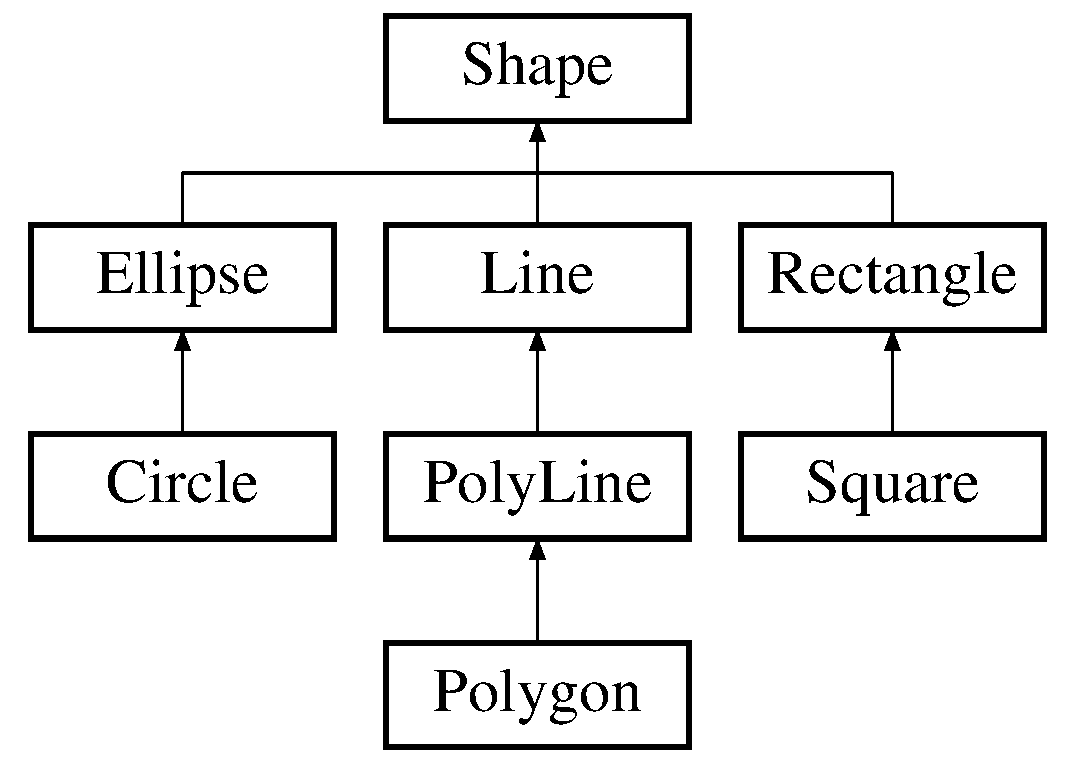
\includegraphics[height=4.000000cm]{class_shape}
\end{center}
\end{figure}
\subsection*{Public Member Functions}
\begin{DoxyCompactItemize}
\item 
\mbox{\Hypertarget{class_shape_ab41921d0dd6e4480d9232e2556991863}\label{class_shape_ab41921d0dd6e4480d9232e2556991863}} 
{\bfseries Shape} (Q\+String id\+In, bool is\+Render, Qt\+::\+Brush\+Style brush\+In, Qt\+::\+Global\+Color pencolor\+In, double width, Qt\+::\+Pen\+Cap\+Style pen\+Cap\+In, Qt\+::\+Pen\+Join\+Style pen\+Join\+In, Qt\+::\+Global\+Color brush\+Color\+In, Qt\+::\+Pen\+Style pen\+Style\+In)
\item 
\mbox{\Hypertarget{class_shape_ae7a27992cf927eb09b31ac38b11f1d8d}\label{class_shape_ae7a27992cf927eb09b31ac38b11f1d8d}} 
{\bfseries Shape} (Q\+String id\+In, bool is\+Render, Q\+String brush\+In, Q\+String pen\+Color\+In, double width, Q\+String pen\+Cap\+In, Q\+String Pen\+Join\+In, Q\+String Brush\+Color\+In, Q\+String Pen\+Style\+In)
\item 
\mbox{\Hypertarget{class_shape_a14489e501cf05219c32ee79e6331d3ef}\label{class_shape_a14489e501cf05219c32ee79e6331d3ef}} 
{\bfseries Shape} (Q\+String id\+In, bool is\+Render, int brush\+In, int pen\+Color\+In, double width, int pen\+Cap\+In, int Pen\+Join\+In, int Brush\+Color\+In, int Pen\+Style\+In)
\item 
\mbox{\Hypertarget{class_shape_a51e4f98296596a66ed673690267f9849}\label{class_shape_a51e4f98296596a66ed673690267f9849}} 
Qt\+::\+Brush\+Style {\bfseries int\+To\+Brush\+Style} (int index)
\item 
\mbox{\Hypertarget{class_shape_a63318b91c48c0184a7cc99567768f6eb}\label{class_shape_a63318b91c48c0184a7cc99567768f6eb}} 
Qt\+::\+Global\+Color {\bfseries int\+To\+Color} (int index)
\item 
\mbox{\Hypertarget{class_shape_ab9a6d3653678500542c6ef83cbf8b68c}\label{class_shape_ab9a6d3653678500542c6ef83cbf8b68c}} 
Qt\+::\+Pen\+Cap\+Style {\bfseries int\+To\+Pen\+Cap} (int index)
\item 
\mbox{\Hypertarget{class_shape_a06bbdbf344d0ecdc764ce59b6a95368d}\label{class_shape_a06bbdbf344d0ecdc764ce59b6a95368d}} 
Qt\+::\+Pen\+Join\+Style {\bfseries int\+To\+Pen\+Join} (int index)
\item 
\mbox{\Hypertarget{class_shape_ad4c0545fbc55a595504dedb0f9d6f6e4}\label{class_shape_ad4c0545fbc55a595504dedb0f9d6f6e4}} 
Qt\+::\+Pen\+Style {\bfseries int\+To\+Pen\+Style} (int index)
\item 
\mbox{\Hypertarget{class_shape_a219c9f9c30588dd10462d7c0a634fad3}\label{class_shape_a219c9f9c30588dd10462d7c0a634fad3}} 
bool {\bfseries is\+Rendered} ()
\item 
\mbox{\Hypertarget{class_shape_a41fd467475c084321064a35e1fdd983f}\label{class_shape_a41fd467475c084321064a35e1fdd983f}} 
void {\bfseries configure\+Painter} (Q\+Painter \&p)
\item 
\mbox{\Hypertarget{class_shape_ab94f8b25d05839c7227c6deddcc48b9f}\label{class_shape_ab94f8b25d05839c7227c6deddcc48b9f}} 
Q\+String {\bfseries Get\+ID} ()
\item 
\mbox{\Hypertarget{class_shape_a9bbe42c30c0393922840703a97016f88}\label{class_shape_a9bbe42c30c0393922840703a97016f88}} 
Q\+String {\bfseries Get\+Pen\+Color} ()
\item 
\mbox{\Hypertarget{class_shape_a936495776867dbfdd5eb7575a13c844d}\label{class_shape_a936495776867dbfdd5eb7575a13c844d}} 
Q\+String {\bfseries Get\+Pen\+Width} ()
\item 
\mbox{\Hypertarget{class_shape_af533bf51d240c2015123b3ea37e21464}\label{class_shape_af533bf51d240c2015123b3ea37e21464}} 
Q\+String {\bfseries Get\+Pen\+Style} ()
\item 
\mbox{\Hypertarget{class_shape_a7273d75f1aa60eab01ee49830ccc4c81}\label{class_shape_a7273d75f1aa60eab01ee49830ccc4c81}} 
Q\+String {\bfseries Get\+Pen\+Cap\+Style} ()
\item 
\mbox{\Hypertarget{class_shape_a3850dedfd2b83302510ba817209ab40f}\label{class_shape_a3850dedfd2b83302510ba817209ab40f}} 
Q\+String {\bfseries Get\+Pen\+Join\+Style} ()
\item 
\mbox{\Hypertarget{class_shape_ace50307bf23aa364eab8f52531a9d35d}\label{class_shape_ace50307bf23aa364eab8f52531a9d35d}} 
Q\+String {\bfseries Get\+Brush\+Color} ()
\item 
\mbox{\Hypertarget{class_shape_a9ff424ba6bc200c826be8a71e6d2727b}\label{class_shape_a9ff424ba6bc200c826be8a71e6d2727b}} 
Q\+String {\bfseries Get\+Brush\+Style} ()
\item 
virtual void \hyperlink{class_shape_a26d57a0589b0fd7ff03a4b5ad8dc530a}{move} (Q\+Point xy)
\begin{DoxyCompactList}\small\item\em move -\/ handles moving the shape and recieves in mouse input \end{DoxyCompactList}\item 
\mbox{\Hypertarget{class_shape_aff9e910aba74bd21a349d358b4aec86a}\label{class_shape_aff9e910aba74bd21a349d358b4aec86a}} 
virtual void {\bfseries move} (int x, int y)
\item 
\mbox{\Hypertarget{class_shape_ab5523ae50b25161b3a64c7728de99e1f}\label{class_shape_ab5523ae50b25161b3a64c7728de99e1f}} 
virtual void {\bfseries resize} (double x)
\item 
virtual void \hyperlink{class_shape_ad7cc6a5e97b0971d50999bce4396127a}{Draw} (\hyperlink{class_canvas}{Canvas} $\ast$paint\+Area)
\begin{DoxyCompactList}\small\item\em Draw -\/ draws the shape\+: virtual. \end{DoxyCompactList}\item 
virtual bool \hyperlink{class_shape_ab2d47c913eb287843e61b2d48e422ced}{is\+\_\+\+Left\+\_\+\+Clicked} (Q\+Point e)
\begin{DoxyCompactList}\small\item\em is\+\_\+\+Left\+\_\+\+Clicked -\/ mouse input \end{DoxyCompactList}\end{DoxyCompactItemize}


\subsection{Detailed Description}
The \hyperlink{class_shape}{Shape} class -\/ base abstract class-\/parent to all other shape classes-\/holds all of the private data types that change or access pen/brush attributes; is also what is held in the shape vector class. 

\subsection{Member Function Documentation}
\mbox{\Hypertarget{class_shape_ad7cc6a5e97b0971d50999bce4396127a}\label{class_shape_ad7cc6a5e97b0971d50999bce4396127a}} 
\index{Shape@{Shape}!Draw@{Draw}}
\index{Draw@{Draw}!Shape@{Shape}}
\subsubsection{\texorpdfstring{Draw()}{Draw()}}
{\footnotesize\ttfamily virtual void Shape\+::\+Draw (\begin{DoxyParamCaption}\item[{\hyperlink{class_canvas}{Canvas} $\ast$}]{paint\+Area }\end{DoxyParamCaption})\hspace{0.3cm}{\ttfamily [inline]}, {\ttfamily [virtual]}}



Draw -\/ draws the shape\+: virtual. 


\begin{DoxyParams}{Parameters}
{\em paint\+Area} & \\
\hline
\end{DoxyParams}


Reimplemented in \hyperlink{class_line_ae645f8a7f03439fa3428f81b1ddb4ffc}{Line}, \hyperlink{class_rectangle_afe989f9ae3ceffd9825b4f1492d764f3}{Rectangle}, \hyperlink{class_circle_a5bebd94955572edce0ad10208a449772}{Circle}, \hyperlink{class_polygon_a9271921d96331c203efcdb50e0ebd64c}{Polygon}, \hyperlink{class_ellipse_aaf9524151dc799501327f72c75e0f010}{Ellipse}, \hyperlink{class_poly_line_ac42ca364849f33b899a929bf57163730}{Poly\+Line}, and \hyperlink{class_square_a30b97f9d3fbd7d226a887ac157b827a0}{Square}.

\mbox{\Hypertarget{class_shape_ab2d47c913eb287843e61b2d48e422ced}\label{class_shape_ab2d47c913eb287843e61b2d48e422ced}} 
\index{Shape@{Shape}!is\+\_\+\+Left\+\_\+\+Clicked@{is\+\_\+\+Left\+\_\+\+Clicked}}
\index{is\+\_\+\+Left\+\_\+\+Clicked@{is\+\_\+\+Left\+\_\+\+Clicked}!Shape@{Shape}}
\subsubsection{\texorpdfstring{is\+\_\+\+Left\+\_\+\+Clicked()}{is\_Left\_Clicked()}}
{\footnotesize\ttfamily virtual bool Shape\+::is\+\_\+\+Left\+\_\+\+Clicked (\begin{DoxyParamCaption}\item[{Q\+Point}]{e }\end{DoxyParamCaption})\hspace{0.3cm}{\ttfamily [inline]}, {\ttfamily [virtual]}}



is\+\_\+\+Left\+\_\+\+Clicked -\/ mouse input 


\begin{DoxyParams}{Parameters}
{\em e} & \\
\hline
\end{DoxyParams}
\begin{DoxyReturn}{Returns}

\end{DoxyReturn}


Reimplemented in \hyperlink{class_line_a79c3891fefd740e6a3cfcdb57a105995}{Line}, \hyperlink{class_rectangle_ade126ee824e394b9c38d2e67a30d1a7d}{Rectangle}, \hyperlink{class_polygon_ab17f2f8ae9489fba4030fbb4a99e7ea6}{Polygon}, \hyperlink{class_circle_a1661bb4e324cce0196a6aa1195c26c73}{Circle}, \hyperlink{class_ellipse_ab3ba6c9f068fc37808778c74f1273f69}{Ellipse}, \hyperlink{class_poly_line_a349f5b14d3ab568ae6776a3d5fd6f956}{Poly\+Line}, and \hyperlink{class_square_aaf0989a3dba67b2502f3a306e0136e69}{Square}.

\mbox{\Hypertarget{class_shape_a26d57a0589b0fd7ff03a4b5ad8dc530a}\label{class_shape_a26d57a0589b0fd7ff03a4b5ad8dc530a}} 
\index{Shape@{Shape}!move@{move}}
\index{move@{move}!Shape@{Shape}}
\subsubsection{\texorpdfstring{move()}{move()}}
{\footnotesize\ttfamily virtual void Shape\+::move (\begin{DoxyParamCaption}\item[{Q\+Point}]{xy }\end{DoxyParamCaption})\hspace{0.3cm}{\ttfamily [inline]}, {\ttfamily [virtual]}}



move -\/ handles moving the shape and recieves in mouse input 


\begin{DoxyParams}{Parameters}
{\em xy} & \\
\hline
\end{DoxyParams}


Reimplemented in \hyperlink{class_circle_a5f02de3ad7e992a689b9f9e88643076c}{Circle}, \hyperlink{class_rectangle_abeeafbc4d44bf241cf655e850f3ce3f3}{Rectangle}, \hyperlink{class_ellipse_a8f5c5a4d8051009fee6d861f163c96dd}{Ellipse}, and \hyperlink{class_square_a49d1e790212e18cb43d7647385cafa20}{Square}.



The documentation for this class was generated from the following files\+:\begin{DoxyCompactItemize}
\item 
shape.\+h\item 
shape.\+cpp\end{DoxyCompactItemize}

\hypertarget{structsingle_user}{}\section{single\+User Struct Reference}
\label{structsingle_user}\index{single\+User@{single\+User}}


The \hyperlink{structsingle_user}{single\+User} struct -\/ user information held in a struct.  




{\ttfamily \#include $<$users.\+h$>$}

\subsection*{Public Attributes}
\begin{DoxyCompactItemize}
\item 
\mbox{\Hypertarget{structsingle_user_a0cab0883de8f6f08c785f96faa0268e6}\label{structsingle_user_a0cab0883de8f6f08c785f96faa0268e6}} 
Q\+String {\bfseries user\+Name}
\item 
\mbox{\Hypertarget{structsingle_user_a155ccd8267749274236b1748066383dc}\label{structsingle_user_a155ccd8267749274236b1748066383dc}} 
Q\+String {\bfseries password}
\item 
\mbox{\Hypertarget{structsingle_user_a2b3b79b107ddc525b1dcd260c1901673}\label{structsingle_user_a2b3b79b107ddc525b1dcd260c1901673}} 
status {\bfseries user\+Status}
\end{DoxyCompactItemize}


\subsection{Detailed Description}
The \hyperlink{structsingle_user}{single\+User} struct -\/ user information held in a struct. 

The documentation for this struct was generated from the following file\+:\begin{DoxyCompactItemize}
\item 
users.\+h\end{DoxyCompactItemize}

\hypertarget{class_square}{}\section{Square Class Reference}
\label{class_square}\index{Square@{Square}}
Inheritance diagram for Square\+:\begin{figure}[H]
\begin{center}
\leavevmode
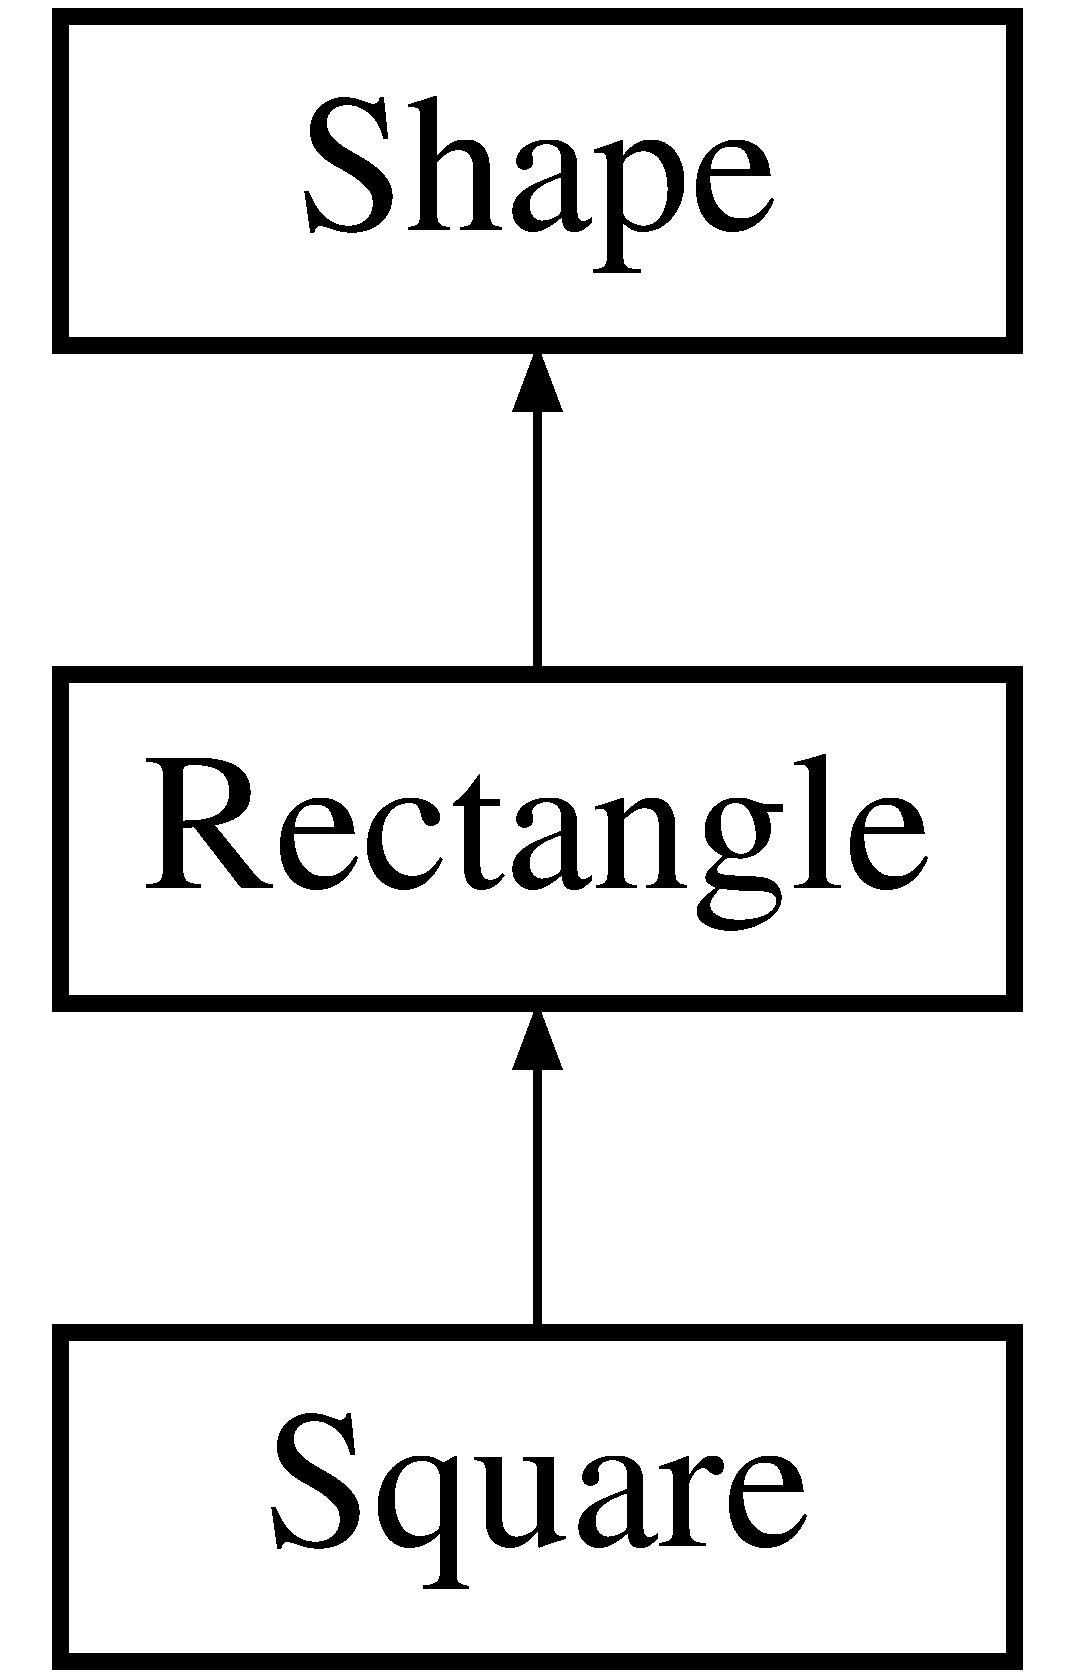
\includegraphics[height=3.000000cm]{class_square}
\end{center}
\end{figure}
\subsection*{Public Member Functions}
\begin{DoxyCompactItemize}
\item 
\mbox{\Hypertarget{class_square_a5f961462240a582c0435860b84b49aa7}\label{class_square_a5f961462240a582c0435860b84b49aa7}} 
{\bfseries Square} (int x, int y, double s)
\item 
\mbox{\Hypertarget{class_square_a467ac8214b403ae54eb70c632710e591}\label{class_square_a467ac8214b403ae54eb70c632710e591}} 
{\bfseries Square} (Q\+String id\+In, Qt\+::\+Brush\+Style brush\+Style\+In, Qt\+::\+Global\+Color brush\+Color\+In, double pen\+Width\+In, Qt\+::\+Global\+Color pen\+Color\+In, Qt\+::\+Pen\+Cap\+Style pen\+Cap\+In, Qt\+::\+Pen\+Join\+Style pen\+Join\+In, Qt\+::\+Pen\+Style pen\+Style\+In, double xR)
\item 
\mbox{\Hypertarget{class_square_a47e8c3e52b0cee679b9d2e3b53ad4da6}\label{class_square_a47e8c3e52b0cee679b9d2e3b53ad4da6}} 
{\bfseries Square} (\hyperlink{class_square}{Square} \&copy)
\item 
\mbox{\Hypertarget{class_square_aa18cd8139b5b19cf95852d4c0801705c}\label{class_square_aa18cd8139b5b19cf95852d4c0801705c}} 
{\bfseries Square} (\hyperlink{class_square}{Square} \&\&copy)
\item 
\mbox{\Hypertarget{class_square_a5f6ea125b5218b4abd87b591d4d3a3b8}\label{class_square_a5f6ea125b5218b4abd87b591d4d3a3b8}} 
void {\bfseries set\+Size} (double s)
\item 
\mbox{\Hypertarget{class_square_a81ac7c0d1056d92aa8e380948f58b76c}\label{class_square_a81ac7c0d1056d92aa8e380948f58b76c}} 
virtual double {\bfseries get\+Area} ()
\item 
\mbox{\Hypertarget{class_square_a7f112541e11aca59b90fa866b3104718}\label{class_square_a7f112541e11aca59b90fa866b3104718}} 
virtual double {\bfseries get\+Perimeter} ()
\item 
virtual void \hyperlink{class_square_a49d1e790212e18cb43d7647385cafa20}{move} (Q\+Point xy)
\begin{DoxyCompactList}\small\item\em move -\/ handles moving the shape and recieves in mouse input \end{DoxyCompactList}\item 
virtual void \hyperlink{class_square_a30b97f9d3fbd7d226a887ac157b827a0}{Draw} (\hyperlink{class_canvas}{Canvas} $\ast$draw\+Area)
\begin{DoxyCompactList}\small\item\em Draw -\/ draws the shape\+: virtual. \end{DoxyCompactList}\item 
virtual bool \hyperlink{class_square_aaf0989a3dba67b2502f3a306e0136e69}{is\+\_\+\+Left\+\_\+\+Clicked} (Q\+Point e)
\begin{DoxyCompactList}\small\item\em is\+\_\+\+Left\+\_\+\+Clicked -\/ mouse input \end{DoxyCompactList}\end{DoxyCompactItemize}


\subsection{Member Function Documentation}
\mbox{\Hypertarget{class_square_a30b97f9d3fbd7d226a887ac157b827a0}\label{class_square_a30b97f9d3fbd7d226a887ac157b827a0}} 
\index{Square@{Square}!Draw@{Draw}}
\index{Draw@{Draw}!Square@{Square}}
\subsubsection{\texorpdfstring{Draw()}{Draw()}}
{\footnotesize\ttfamily void Square\+::\+Draw (\begin{DoxyParamCaption}\item[{\hyperlink{class_canvas}{Canvas} $\ast$}]{paint\+Area }\end{DoxyParamCaption})\hspace{0.3cm}{\ttfamily [virtual]}}



Draw -\/ draws the shape\+: virtual. 


\begin{DoxyParams}{Parameters}
{\em paint\+Area} & \\
\hline
\end{DoxyParams}


Reimplemented from \hyperlink{class_rectangle_afe989f9ae3ceffd9825b4f1492d764f3}{Rectangle}.

\mbox{\Hypertarget{class_square_aaf0989a3dba67b2502f3a306e0136e69}\label{class_square_aaf0989a3dba67b2502f3a306e0136e69}} 
\index{Square@{Square}!is\+\_\+\+Left\+\_\+\+Clicked@{is\+\_\+\+Left\+\_\+\+Clicked}}
\index{is\+\_\+\+Left\+\_\+\+Clicked@{is\+\_\+\+Left\+\_\+\+Clicked}!Square@{Square}}
\subsubsection{\texorpdfstring{is\+\_\+\+Left\+\_\+\+Clicked()}{is\_Left\_Clicked()}}
{\footnotesize\ttfamily bool Square\+::is\+\_\+\+Left\+\_\+\+Clicked (\begin{DoxyParamCaption}\item[{Q\+Point}]{e }\end{DoxyParamCaption})\hspace{0.3cm}{\ttfamily [virtual]}}



is\+\_\+\+Left\+\_\+\+Clicked -\/ mouse input 


\begin{DoxyParams}{Parameters}
{\em e} & \\
\hline
\end{DoxyParams}
\begin{DoxyReturn}{Returns}

\end{DoxyReturn}


Reimplemented from \hyperlink{class_rectangle_ade126ee824e394b9c38d2e67a30d1a7d}{Rectangle}.

\mbox{\Hypertarget{class_square_a49d1e790212e18cb43d7647385cafa20}\label{class_square_a49d1e790212e18cb43d7647385cafa20}} 
\index{Square@{Square}!move@{move}}
\index{move@{move}!Square@{Square}}
\subsubsection{\texorpdfstring{move()}{move()}}
{\footnotesize\ttfamily void Square\+::move (\begin{DoxyParamCaption}\item[{Q\+Point}]{xy }\end{DoxyParamCaption})\hspace{0.3cm}{\ttfamily [virtual]}}



move -\/ handles moving the shape and recieves in mouse input 


\begin{DoxyParams}{Parameters}
{\em xy} & \\
\hline
\end{DoxyParams}


Reimplemented from \hyperlink{class_rectangle_abeeafbc4d44bf241cf655e850f3ce3f3}{Rectangle}.



The documentation for this class was generated from the following files\+:\begin{DoxyCompactItemize}
\item 
Square.\+h\item 
Square.\+cpp\end{DoxyCompactItemize}

\hypertarget{class_ui_1_1_testimonials}{}\section{Ui\+:\+:Testimonials Class Reference}
\label{class_ui_1_1_testimonials}\index{Ui\+::\+Testimonials@{Ui\+::\+Testimonials}}
Inheritance diagram for Ui\+:\+:Testimonials\+:\begin{figure}[H]
\begin{center}
\leavevmode
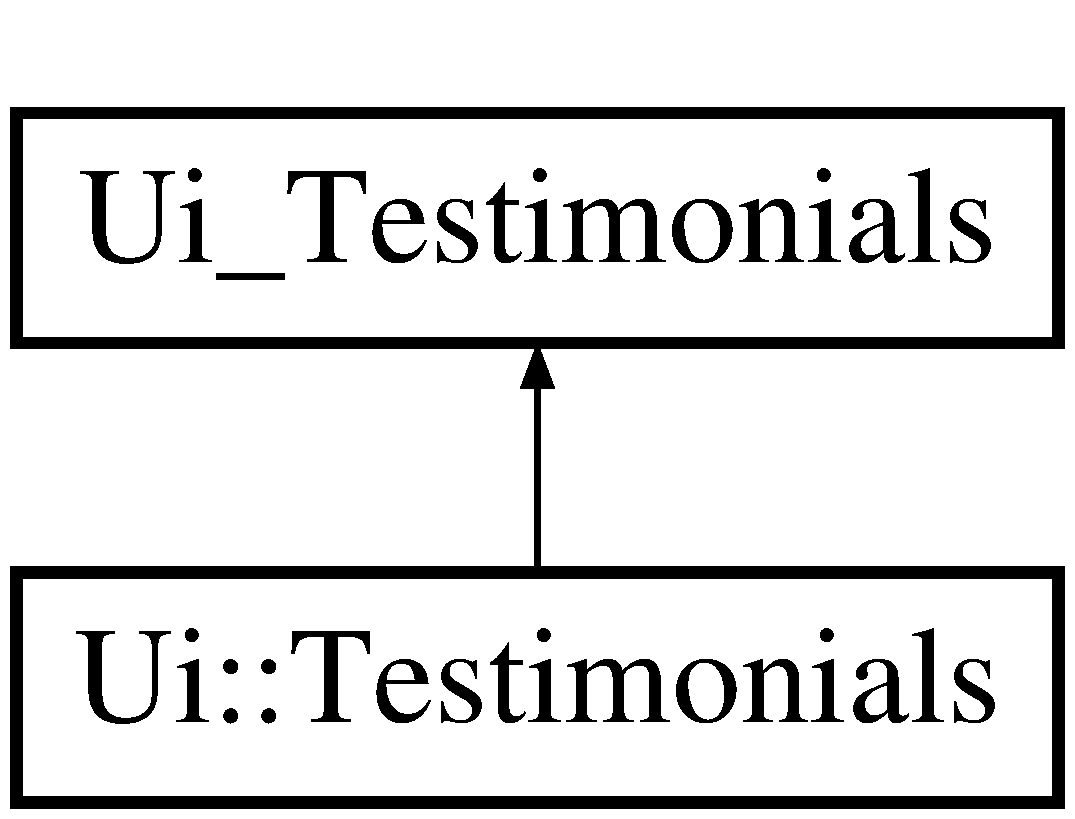
\includegraphics[height=2.000000cm]{class_ui_1_1_testimonials}
\end{center}
\end{figure}
\subsection*{Additional Inherited Members}


The documentation for this class was generated from the following file\+:\begin{DoxyCompactItemize}
\item 
ui\+\_\+testimonials.\+h\end{DoxyCompactItemize}

\hypertarget{class_testimonials}{}\section{Testimonials Class Reference}
\label{class_testimonials}\index{Testimonials@{Testimonials}}
Inheritance diagram for Testimonials\+:\begin{figure}[H]
\begin{center}
\leavevmode
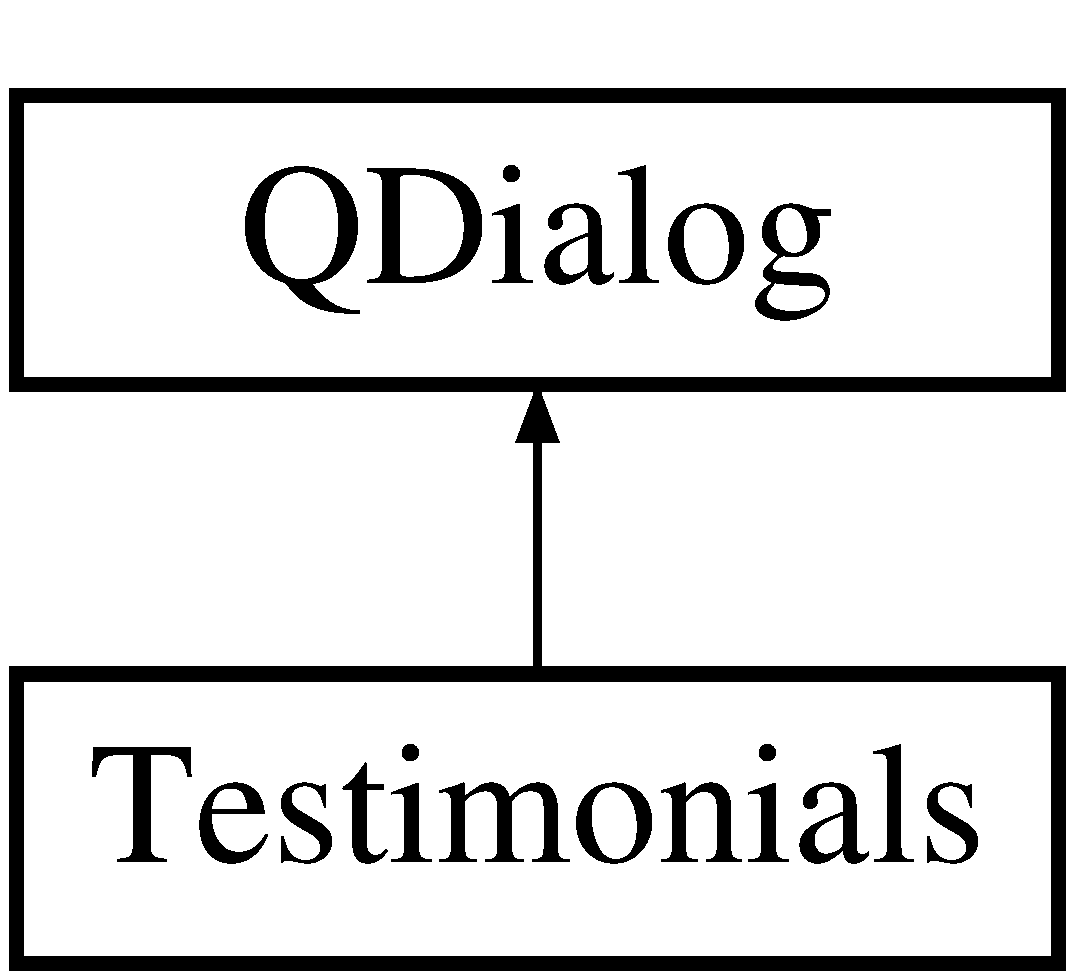
\includegraphics[height=2.000000cm]{class_testimonials}
\end{center}
\end{figure}
\subsection*{Public Member Functions}
\begin{DoxyCompactItemize}
\item 
\mbox{\Hypertarget{class_testimonials_a7fd3351a059293a49dc50907b1e1ab04}\label{class_testimonials_a7fd3351a059293a49dc50907b1e1ab04}} 
{\bfseries Testimonials} (Q\+Widget $\ast$parent=0)
\end{DoxyCompactItemize}


The documentation for this class was generated from the following files\+:\begin{DoxyCompactItemize}
\item 
testimonials.\+h\item 
testimonials.\+cpp\end{DoxyCompactItemize}

\hypertarget{class_ui___contact}{}\section{Ui\+\_\+\+Contact Class Reference}
\label{class_ui___contact}\index{Ui\+\_\+\+Contact@{Ui\+\_\+\+Contact}}
Inheritance diagram for Ui\+\_\+\+Contact\+:\begin{figure}[H]
\begin{center}
\leavevmode
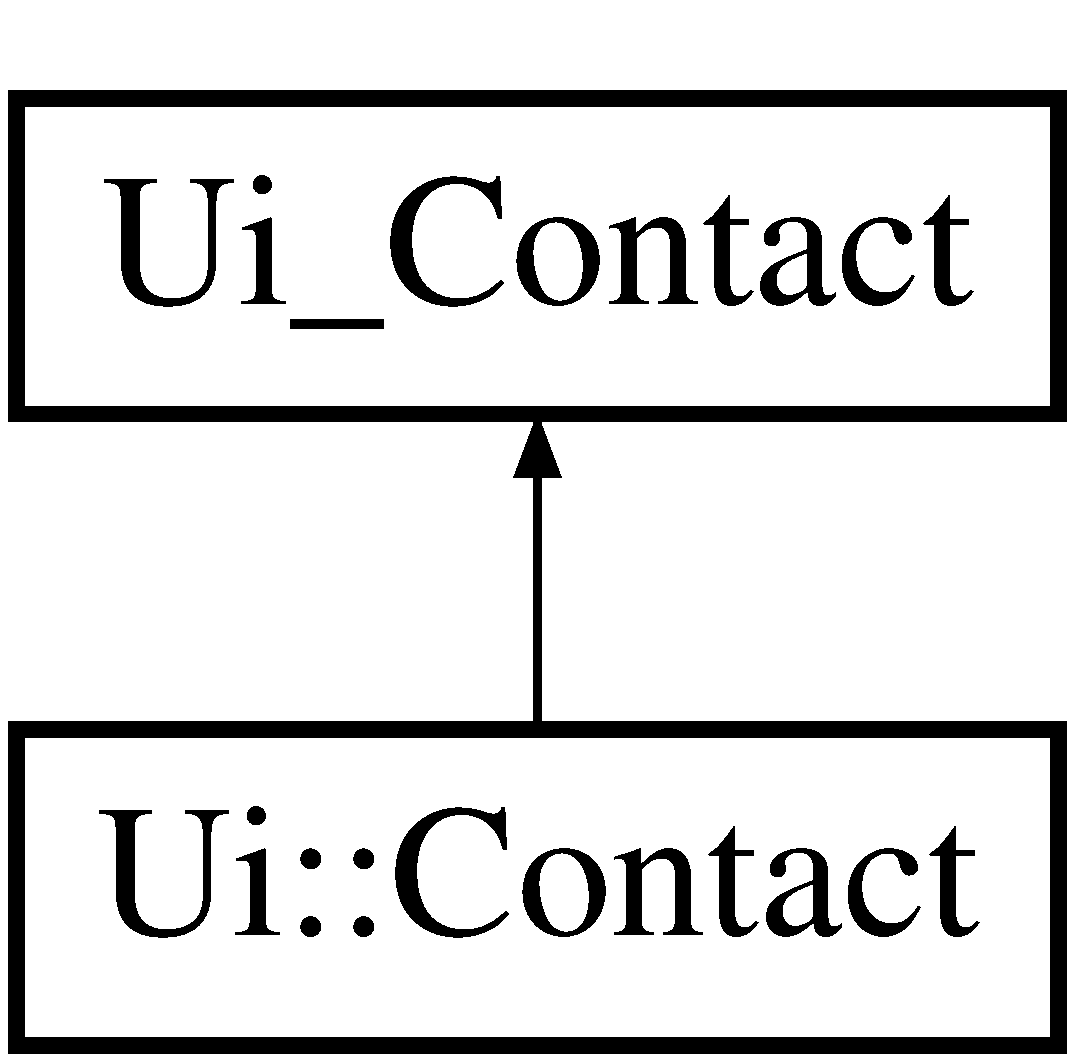
\includegraphics[height=2.000000cm]{class_ui___contact}
\end{center}
\end{figure}
\subsection*{Public Member Functions}
\begin{DoxyCompactItemize}
\item 
\mbox{\Hypertarget{class_ui___contact_ac731f4f9be5756a93ce6e2020d6bb103}\label{class_ui___contact_ac731f4f9be5756a93ce6e2020d6bb103}} 
void {\bfseries setup\+Ui} (Q\+Dialog $\ast$\hyperlink{class_contact}{Contact})
\item 
\mbox{\Hypertarget{class_ui___contact_a733b9a62964ac18185c9eb9097f689f4}\label{class_ui___contact_a733b9a62964ac18185c9eb9097f689f4}} 
void {\bfseries retranslate\+Ui} (Q\+Dialog $\ast$\hyperlink{class_contact}{Contact})
\end{DoxyCompactItemize}
\subsection*{Public Attributes}
\begin{DoxyCompactItemize}
\item 
\mbox{\Hypertarget{class_ui___contact_a5aae395305d53fdcb3ed259d9dc6e317}\label{class_ui___contact_a5aae395305d53fdcb3ed259d9dc6e317}} 
Q\+Label $\ast$ {\bfseries Contact\+Us\+Image}
\end{DoxyCompactItemize}


The documentation for this class was generated from the following file\+:\begin{DoxyCompactItemize}
\item 
ui\+\_\+contact.\+h\end{DoxyCompactItemize}

\hypertarget{class_ui___dialog}{}\section{Ui\+\_\+\+Dialog Class Reference}
\label{class_ui___dialog}\index{Ui\+\_\+\+Dialog@{Ui\+\_\+\+Dialog}}
Inheritance diagram for Ui\+\_\+\+Dialog\+:\begin{figure}[H]
\begin{center}
\leavevmode
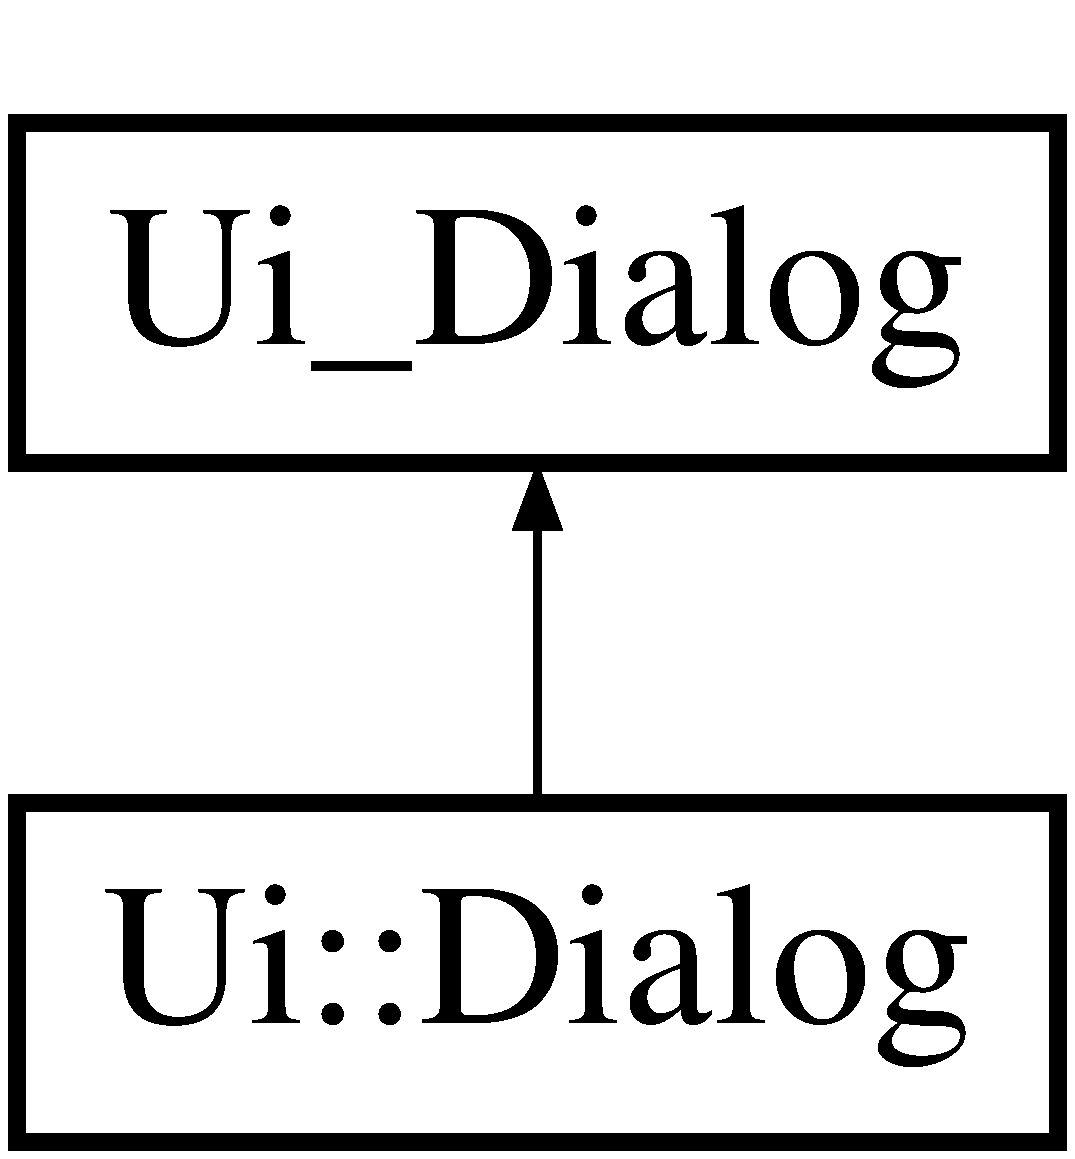
\includegraphics[height=2.000000cm]{class_ui___dialog}
\end{center}
\end{figure}
\subsection*{Public Member Functions}
\begin{DoxyCompactItemize}
\item 
\mbox{\Hypertarget{class_ui___dialog_a4f6a478c3ecdafabffb17b39cb26444a}\label{class_ui___dialog_a4f6a478c3ecdafabffb17b39cb26444a}} 
void {\bfseries setup\+Ui} (Q\+Dialog $\ast$Dialog)
\item 
\mbox{\Hypertarget{class_ui___dialog_afa0ccb6f716ca6178260522a193c250e}\label{class_ui___dialog_afa0ccb6f716ca6178260522a193c250e}} 
void {\bfseries retranslate\+Ui} (Q\+Dialog $\ast$Dialog)
\end{DoxyCompactItemize}
\subsection*{Public Attributes}
\begin{DoxyCompactItemize}
\item 
\mbox{\Hypertarget{class_ui___dialog_aaf3cec313cf0b690af7c430773fe3c72}\label{class_ui___dialog_aaf3cec313cf0b690af7c430773fe3c72}} 
Q\+Tab\+Widget $\ast$ {\bfseries Tabs}
\item 
\mbox{\Hypertarget{class_ui___dialog_a4d635d50856f18798cb5cf08e1d29cdb}\label{class_ui___dialog_a4d635d50856f18798cb5cf08e1d29cdb}} 
Q\+Widget $\ast$ {\bfseries Canvas}
\item 
\mbox{\Hypertarget{class_ui___dialog_ac29d40a685ece2dc888a3e37594dbc15}\label{class_ui___dialog_ac29d40a685ece2dc888a3e37594dbc15}} 
Q\+Widget $\ast$ {\bfseries widget}
\item 
\mbox{\Hypertarget{class_ui___dialog_ae66a1da203f045e33d71ed5abd46d2a1}\label{class_ui___dialog_ae66a1da203f045e33d71ed5abd46d2a1}} 
Q\+H\+Box\+Layout $\ast$ {\bfseries horizontal\+Layout}
\item 
\mbox{\Hypertarget{class_ui___dialog_afe391e90b26eb23a2b08f0b51dc288b9}\label{class_ui___dialog_afe391e90b26eb23a2b08f0b51dc288b9}} 
Q\+Splitter $\ast$ {\bfseries Canvas\+Info\+Splitter}
\item 
\mbox{\Hypertarget{class_ui___dialog_a05a3e0ba3f3d95c4531c4c2854d2b3f9}\label{class_ui___dialog_a05a3e0ba3f3d95c4531c4c2854d2b3f9}} 
Q\+Splitter $\ast$ {\bfseries Mod\+Splitter}
\item 
\mbox{\Hypertarget{class_ui___dialog_a2ddd3ee48dcfafec3c95f63646adcbb0}\label{class_ui___dialog_a2ddd3ee48dcfafec3c95f63646adcbb0}} 
Q\+Widget $\ast$ {\bfseries widget1}
\item 
\mbox{\Hypertarget{class_ui___dialog_a4fb6d1c8d4780f0d513f4a48af4a2b10}\label{class_ui___dialog_a4fb6d1c8d4780f0d513f4a48af4a2b10}} 
Q\+V\+Box\+Layout $\ast$ {\bfseries vertical\+Layout\+\_\+2}
\item 
\mbox{\Hypertarget{class_ui___dialog_a1ef2dfac27a834aebbc5bef21d7cba90}\label{class_ui___dialog_a1ef2dfac27a834aebbc5bef21d7cba90}} 
Q\+Label $\ast$ {\bfseries shape\+Id\+Label}
\item 
\mbox{\Hypertarget{class_ui___dialog_a0b42046688bafe558289042b4cd523fd}\label{class_ui___dialog_a0b42046688bafe558289042b4cd523fd}} 
Q\+Label $\ast$ {\bfseries pen\+Color\+Label}
\item 
\mbox{\Hypertarget{class_ui___dialog_a0489922a5c4636c122a51a72748aba31}\label{class_ui___dialog_a0489922a5c4636c122a51a72748aba31}} 
Q\+Label $\ast$ {\bfseries pen\+Width\+Label}
\item 
\mbox{\Hypertarget{class_ui___dialog_a7ea8c521963f4e57020c785a3496487b}\label{class_ui___dialog_a7ea8c521963f4e57020c785a3496487b}} 
Q\+Label $\ast$ {\bfseries pen\+Style\+Label}
\item 
\mbox{\Hypertarget{class_ui___dialog_aee9cf4313d578a68c044121db4922546}\label{class_ui___dialog_aee9cf4313d578a68c044121db4922546}} 
Q\+Label $\ast$ {\bfseries pen\+Cap\+Style\+Label}
\item 
\mbox{\Hypertarget{class_ui___dialog_a26b119be9cb3883db5eebb6e504d4b68}\label{class_ui___dialog_a26b119be9cb3883db5eebb6e504d4b68}} 
Q\+Label $\ast$ {\bfseries Pen\+Join\+Label}
\item 
\mbox{\Hypertarget{class_ui___dialog_a03fad8997ac8dd2e1dcbda128a2bae77}\label{class_ui___dialog_a03fad8997ac8dd2e1dcbda128a2bae77}} 
Q\+Label $\ast$ {\bfseries Brush\+Color\+Label}
\item 
\mbox{\Hypertarget{class_ui___dialog_a78b67fc4feacfa6ab4cf420c7701f247}\label{class_ui___dialog_a78b67fc4feacfa6ab4cf420c7701f247}} 
Q\+Label $\ast$ {\bfseries brush\+Style\+Label}
\item 
\mbox{\Hypertarget{class_ui___dialog_acb48eea35355758b711f08dac127a9e1}\label{class_ui___dialog_acb48eea35355758b711f08dac127a9e1}} 
Q\+Widget $\ast$ {\bfseries widget2}
\item 
\mbox{\Hypertarget{class_ui___dialog_aa9f412da1b6a4d0aa29766400870b8fa}\label{class_ui___dialog_aa9f412da1b6a4d0aa29766400870b8fa}} 
Q\+V\+Box\+Layout $\ast$ {\bfseries Input\+Layout}
\item 
\mbox{\Hypertarget{class_ui___dialog_a72b66b075a78a59b299da234c845fc6f}\label{class_ui___dialog_a72b66b075a78a59b299da234c845fc6f}} 
Q\+Line\+Edit $\ast$ {\bfseries shape\+Id\+Edit}
\item 
\mbox{\Hypertarget{class_ui___dialog_ad1bb04253a4c38c13b5fc473806413cd}\label{class_ui___dialog_ad1bb04253a4c38c13b5fc473806413cd}} 
Q\+Combo\+Box $\ast$ {\bfseries pen\+Color\+Edit}
\item 
\mbox{\Hypertarget{class_ui___dialog_a2b72410577bab765668edd17761d0a16}\label{class_ui___dialog_a2b72410577bab765668edd17761d0a16}} 
Q\+Slider $\ast$ {\bfseries pen\+Width\+Edit}
\item 
\mbox{\Hypertarget{class_ui___dialog_a10803aefb72747c9aa55a67e9e744167}\label{class_ui___dialog_a10803aefb72747c9aa55a67e9e744167}} 
Q\+Combo\+Box $\ast$ {\bfseries pen\+Style\+Edit}
\item 
\mbox{\Hypertarget{class_ui___dialog_a43f9148f84a766ec36822004a430e51d}\label{class_ui___dialog_a43f9148f84a766ec36822004a430e51d}} 
Q\+Combo\+Box $\ast$ {\bfseries Pen\+Cap\+Edit}
\item 
\mbox{\Hypertarget{class_ui___dialog_ac589d33c987fb9a7ecc6b6de683f2882}\label{class_ui___dialog_ac589d33c987fb9a7ecc6b6de683f2882}} 
Q\+Combo\+Box $\ast$ {\bfseries Pen\+Join\+Edit}
\item 
\mbox{\Hypertarget{class_ui___dialog_a624f6731f87db942d68eca53f0c06e25}\label{class_ui___dialog_a624f6731f87db942d68eca53f0c06e25}} 
Q\+Combo\+Box $\ast$ {\bfseries brush\+Color\+Edit}
\item 
\mbox{\Hypertarget{class_ui___dialog_afd29a2d70334893b6d177c9a57f33b6b}\label{class_ui___dialog_afd29a2d70334893b6d177c9a57f33b6b}} 
Q\+Combo\+Box $\ast$ {\bfseries brush\+Style\+Edit}
\item 
\mbox{\Hypertarget{class_ui___dialog_af2ecd6be4b8d7b0f0c7685a608d13656}\label{class_ui___dialog_af2ecd6be4b8d7b0f0c7685a608d13656}} 
Q\+Table\+Widget $\ast$ {\bfseries layer\+Table}
\item 
\mbox{\Hypertarget{class_ui___dialog_a95e25d36a940c3e3e4a684c7dea1dece}\label{class_ui___dialog_a95e25d36a940c3e3e4a684c7dea1dece}} 
Q\+Graphics\+View $\ast$ {\bfseries graphics\+View}
\item 
\mbox{\Hypertarget{class_ui___dialog_a9c68cd2b3268c177e82f4a7ad317009d}\label{class_ui___dialog_a9c68cd2b3268c177e82f4a7ad317009d}} 
Q\+Widget $\ast$ {\bfseries Table}
\item 
\mbox{\Hypertarget{class_ui___dialog_a87b7964eb92867741cdb514cfbbbddbb}\label{class_ui___dialog_a87b7964eb92867741cdb514cfbbbddbb}} 
Q\+Table\+Widget $\ast$ {\bfseries table\+Widget}
\item 
\mbox{\Hypertarget{class_ui___dialog_aa53861d342d8fc315ddb095541f9115f}\label{class_ui___dialog_aa53861d342d8fc315ddb095541f9115f}} 
Q\+Widget $\ast$ {\bfseries About}
\item 
\mbox{\Hypertarget{class_ui___dialog_ada792e4089e6aa0034786baecfe27854}\label{class_ui___dialog_ada792e4089e6aa0034786baecfe27854}} 
Q\+Label $\ast$ {\bfseries contact\+Us\+Label}
\item 
\mbox{\Hypertarget{class_ui___dialog_a6502473db1f2a5c6a1f3f8a1415ee404}\label{class_ui___dialog_a6502473db1f2a5c6a1f3f8a1415ee404}} 
Q\+Label $\ast$ {\bfseries mainenance\+Plan\+Label}
\item 
\mbox{\Hypertarget{class_ui___dialog_aa47dad1533d0a5db4aca7c604378210c}\label{class_ui___dialog_aa47dad1533d0a5db4aca7c604378210c}} 
Q\+Label $\ast$ {\bfseries testimonials\+Label}
\end{DoxyCompactItemize}


The documentation for this class was generated from the following file\+:\begin{DoxyCompactItemize}
\item 
ui\+\_\+dialog.\+h\end{DoxyCompactItemize}

\hypertarget{class_ui___help}{}\section{Ui\+\_\+\+Help Class Reference}
\label{class_ui___help}\index{Ui\+\_\+\+Help@{Ui\+\_\+\+Help}}
Inheritance diagram for Ui\+\_\+\+Help\+:\begin{figure}[H]
\begin{center}
\leavevmode
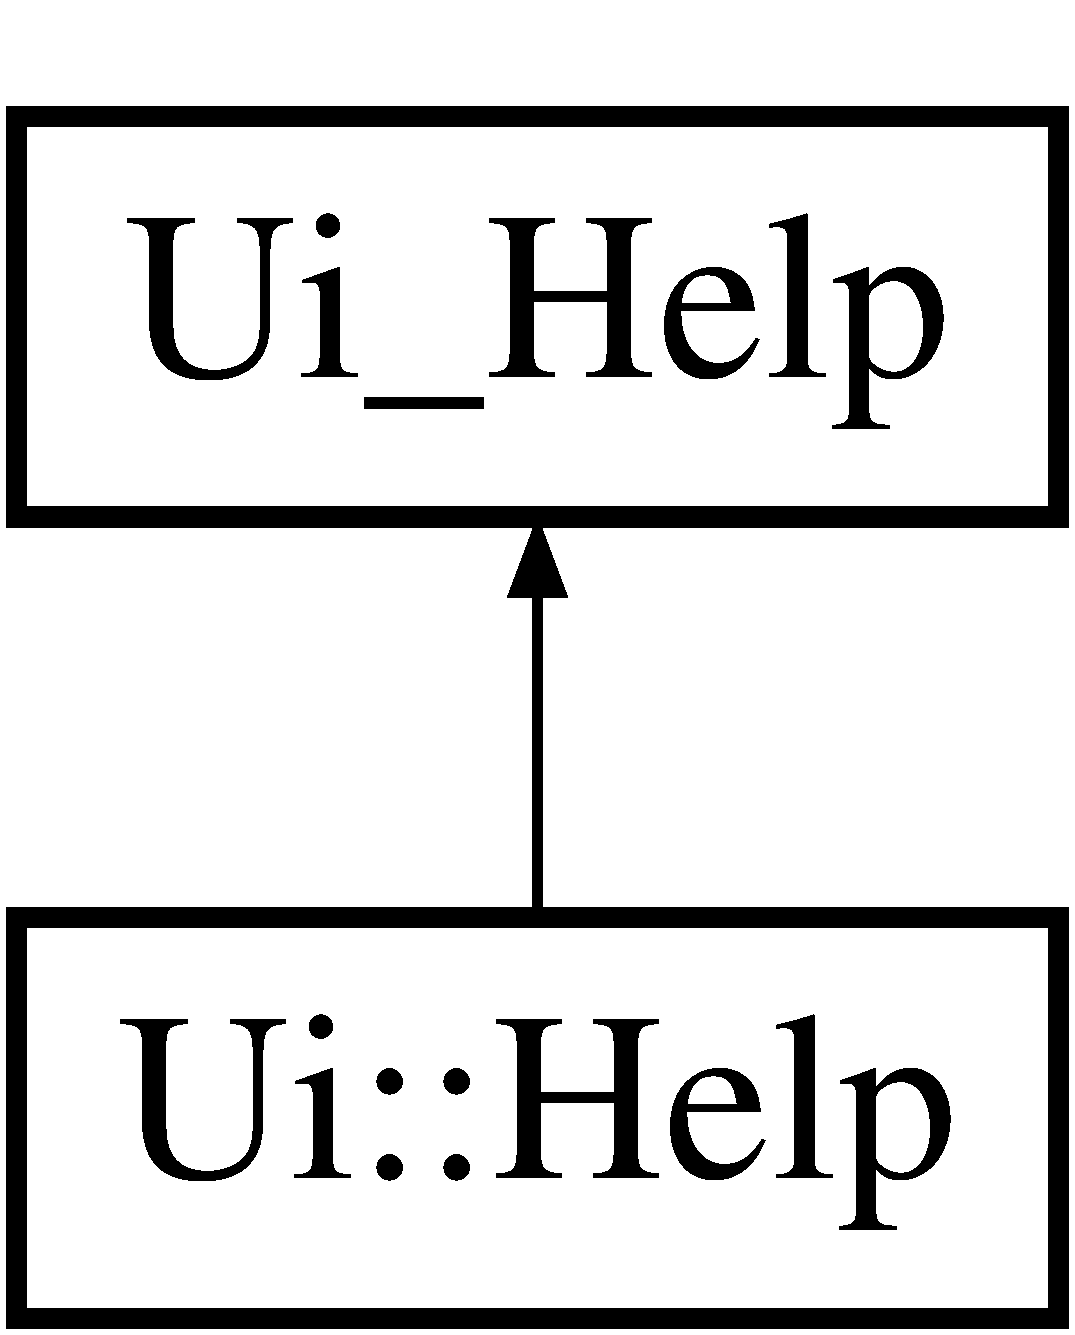
\includegraphics[height=2.000000cm]{class_ui___help}
\end{center}
\end{figure}
\subsection*{Public Member Functions}
\begin{DoxyCompactItemize}
\item 
\mbox{\Hypertarget{class_ui___help_acd2c60ca2345d1ab4c5c9c770071a024}\label{class_ui___help_acd2c60ca2345d1ab4c5c9c770071a024}} 
void {\bfseries setup\+Ui} (Q\+Dialog $\ast$\hyperlink{class_help}{Help})
\item 
\mbox{\Hypertarget{class_ui___help_a7d7ecfed16238fc52df88526d132281a}\label{class_ui___help_a7d7ecfed16238fc52df88526d132281a}} 
void {\bfseries retranslate\+Ui} (Q\+Dialog $\ast$\hyperlink{class_help}{Help})
\end{DoxyCompactItemize}


The documentation for this class was generated from the following file\+:\begin{DoxyCompactItemize}
\item 
ui\+\_\+help.\+h\end{DoxyCompactItemize}

\hypertarget{class_ui___login_screen}{}\section{Ui\+\_\+\+Login\+Screen Class Reference}
\label{class_ui___login_screen}\index{Ui\+\_\+\+Login\+Screen@{Ui\+\_\+\+Login\+Screen}}
Inheritance diagram for Ui\+\_\+\+Login\+Screen\+:\begin{figure}[H]
\begin{center}
\leavevmode
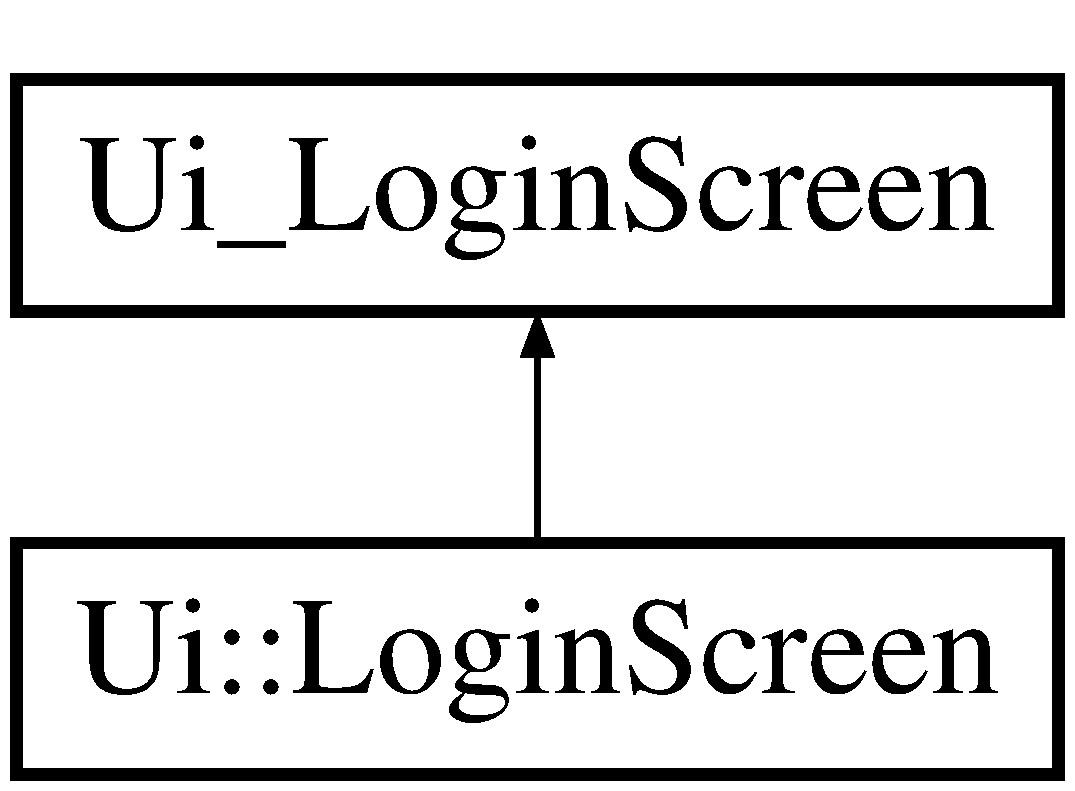
\includegraphics[height=2.000000cm]{class_ui___login_screen}
\end{center}
\end{figure}
\subsection*{Public Member Functions}
\begin{DoxyCompactItemize}
\item 
\mbox{\Hypertarget{class_ui___login_screen_a7ee8dae8b1e23e9bc066986d70b4e777}\label{class_ui___login_screen_a7ee8dae8b1e23e9bc066986d70b4e777}} 
void {\bfseries setup\+Ui} (Q\+Main\+Window $\ast$\hyperlink{class_login_screen}{Login\+Screen})
\item 
\mbox{\Hypertarget{class_ui___login_screen_a7eaabd72044e6593d91fed48e64ef8ee}\label{class_ui___login_screen_a7eaabd72044e6593d91fed48e64ef8ee}} 
void {\bfseries retranslate\+Ui} (Q\+Main\+Window $\ast$\hyperlink{class_login_screen}{Login\+Screen})
\end{DoxyCompactItemize}
\subsection*{Public Attributes}
\begin{DoxyCompactItemize}
\item 
\mbox{\Hypertarget{class_ui___login_screen_a40462e252ed1ffc7c9e7e812aa290a0f}\label{class_ui___login_screen_a40462e252ed1ffc7c9e7e812aa290a0f}} 
Q\+Widget $\ast$ {\bfseries centralwidget}
\item 
\mbox{\Hypertarget{class_ui___login_screen_a4eb43808b9b135ae663749e77efa2eb5}\label{class_ui___login_screen_a4eb43808b9b135ae663749e77efa2eb5}} 
Q\+V\+Box\+Layout $\ast$ {\bfseries vertical\+Layout\+\_\+2}
\item 
\mbox{\Hypertarget{class_ui___login_screen_a38c2ed52ed08bf30ea0f3695227a7f83}\label{class_ui___login_screen_a38c2ed52ed08bf30ea0f3695227a7f83}} 
Q\+Label $\ast$ {\bfseries Logo}
\item 
\mbox{\Hypertarget{class_ui___login_screen_ac304fd0baf53ebc2795ddd481bbff9a1}\label{class_ui___login_screen_ac304fd0baf53ebc2795ddd481bbff9a1}} 
Q\+V\+Box\+Layout $\ast$ {\bfseries vertical\+Layout}
\item 
\mbox{\Hypertarget{class_ui___login_screen_a91a1b61acdf08f7abefc866281620491}\label{class_ui___login_screen_a91a1b61acdf08f7abefc866281620491}} 
Q\+Label $\ast$ {\bfseries name\+\_\+\+Label}
\item 
\mbox{\Hypertarget{class_ui___login_screen_a2a2cdcf7345e76672a0aa5de02981731}\label{class_ui___login_screen_a2a2cdcf7345e76672a0aa5de02981731}} 
Q\+Line\+Edit $\ast$ {\bfseries user\+Name\+Edit}
\item 
\mbox{\Hypertarget{class_ui___login_screen_a22dee7a85929e77bfdaac058da69d39f}\label{class_ui___login_screen_a22dee7a85929e77bfdaac058da69d39f}} 
Q\+Label $\ast$ {\bfseries pass\+\_\+\+Label}
\item 
\mbox{\Hypertarget{class_ui___login_screen_abf63695109a7c991b04d3448fb4a2540}\label{class_ui___login_screen_abf63695109a7c991b04d3448fb4a2540}} 
Q\+Line\+Edit $\ast$ {\bfseries password\+Edit}
\item 
\mbox{\Hypertarget{class_ui___login_screen_aec3646d4f5a8890284ab4c259d6fc196}\label{class_ui___login_screen_aec3646d4f5a8890284ab4c259d6fc196}} 
Q\+V\+Box\+Layout $\ast$ {\bfseries Button\+Layout}
\item 
\mbox{\Hypertarget{class_ui___login_screen_a832a50176fa16cf14569a0ce8a14235c}\label{class_ui___login_screen_a832a50176fa16cf14569a0ce8a14235c}} 
Q\+Push\+Button $\ast$ {\bfseries push\+Button}
\item 
\mbox{\Hypertarget{class_ui___login_screen_afdae720dc03ff1676db9f1ccf399db73}\label{class_ui___login_screen_afdae720dc03ff1676db9f1ccf399db73}} 
Q\+Push\+Button $\ast$ {\bfseries login\+Button}
\item 
\mbox{\Hypertarget{class_ui___login_screen_a202e5d280c74f83c73128f2baaabbbd4}\label{class_ui___login_screen_a202e5d280c74f83c73128f2baaabbbd4}} 
Q\+Menu\+Bar $\ast$ {\bfseries menubar}
\item 
\mbox{\Hypertarget{class_ui___login_screen_abf4c2a355b73009684a94574f58db42b}\label{class_ui___login_screen_abf4c2a355b73009684a94574f58db42b}} 
Q\+Status\+Bar $\ast$ {\bfseries statusbar}
\end{DoxyCompactItemize}


The documentation for this class was generated from the following file\+:\begin{DoxyCompactItemize}
\item 
ui\+\_\+loginscreen.\+h\end{DoxyCompactItemize}

\hypertarget{class_ui___main_interface}{}\section{Ui\+\_\+\+Main\+Interface Class Reference}
\label{class_ui___main_interface}\index{Ui\+\_\+\+Main\+Interface@{Ui\+\_\+\+Main\+Interface}}
Inheritance diagram for Ui\+\_\+\+Main\+Interface\+:\begin{figure}[H]
\begin{center}
\leavevmode
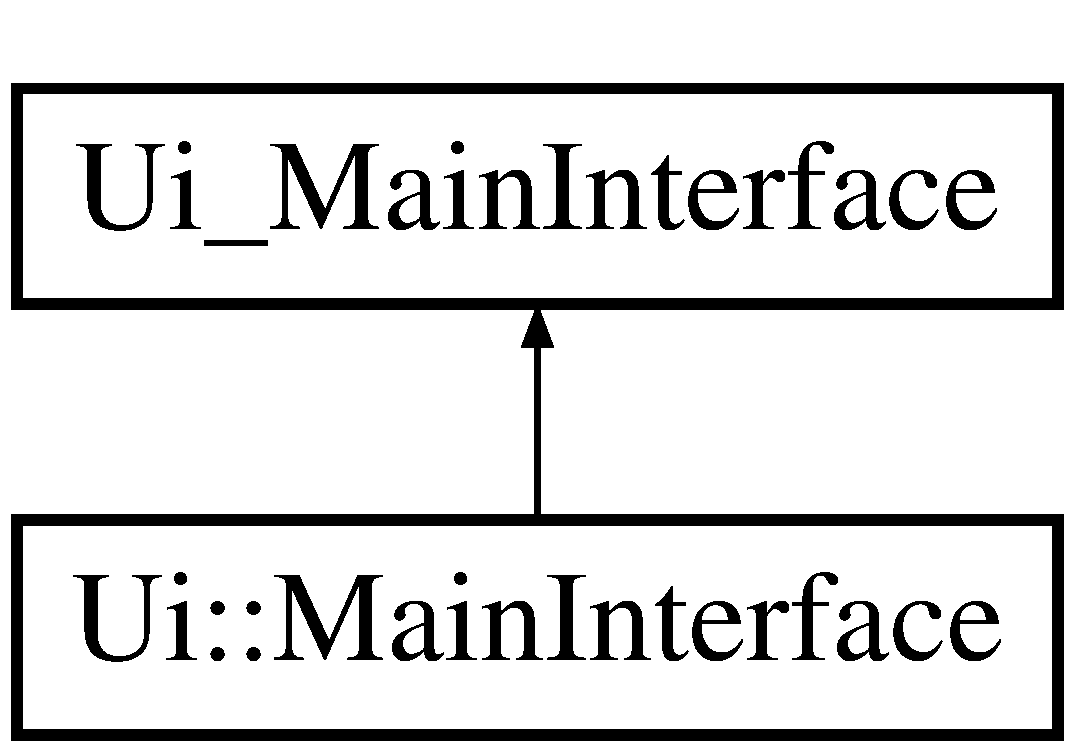
\includegraphics[height=2.000000cm]{class_ui___main_interface}
\end{center}
\end{figure}
\subsection*{Public Member Functions}
\begin{DoxyCompactItemize}
\item 
\mbox{\Hypertarget{class_ui___main_interface_aa8c09ad8ab5464eed7fe57eb946de29e}\label{class_ui___main_interface_aa8c09ad8ab5464eed7fe57eb946de29e}} 
void {\bfseries setup\+Ui} (Q\+Main\+Window $\ast$\hyperlink{class_main_interface}{Main\+Interface})
\item 
\mbox{\Hypertarget{class_ui___main_interface_a6650721ee7cf20dc3178cd34048985ad}\label{class_ui___main_interface_a6650721ee7cf20dc3178cd34048985ad}} 
void {\bfseries retranslate\+Ui} (Q\+Main\+Window $\ast$\hyperlink{class_main_interface}{Main\+Interface})
\end{DoxyCompactItemize}
\subsection*{Public Attributes}
\begin{DoxyCompactItemize}
\item 
\mbox{\Hypertarget{class_ui___main_interface_a9d2b6c149b5fada39615c21aa3399441}\label{class_ui___main_interface_a9d2b6c149b5fada39615c21aa3399441}} 
Q\+Action $\ast$ {\bfseries action\+Maintenance\+\_\+\+Notes}
\item 
\mbox{\Hypertarget{class_ui___main_interface_a1a299a21f63ae8ede45dfe62b197947b}\label{class_ui___main_interface_a1a299a21f63ae8ede45dfe62b197947b}} 
Q\+Action $\ast$ {\bfseries action\+Testimonials}
\item 
\mbox{\Hypertarget{class_ui___main_interface_a7291a03e18714f2fa43e96e0a9d97a28}\label{class_ui___main_interface_a7291a03e18714f2fa43e96e0a9d97a28}} 
Q\+Action $\ast$ {\bfseries action\+Contact\+\_\+\+Us}
\item 
\mbox{\Hypertarget{class_ui___main_interface_a35fd4e52d3fc3d7dfd571528a093b99d}\label{class_ui___main_interface_a35fd4e52d3fc3d7dfd571528a093b99d}} 
Q\+Action $\ast$ {\bfseries action\+T\+BD}
\item 
\mbox{\Hypertarget{class_ui___main_interface_ac4581fec61d5eb396493d874e7ce7bca}\label{class_ui___main_interface_ac4581fec61d5eb396493d874e7ce7bca}} 
Q\+Action $\ast$ {\bfseries action\+Save}
\item 
\mbox{\Hypertarget{class_ui___main_interface_a21261b4111b9df207ac7e1fc06c554a4}\label{class_ui___main_interface_a21261b4111b9df207ac7e1fc06c554a4}} 
Q\+Action $\ast$ {\bfseries action\+Save\+\_\+\+As}
\item 
\mbox{\Hypertarget{class_ui___main_interface_a970cb160ac8300579b41f327155ace58}\label{class_ui___main_interface_a970cb160ac8300579b41f327155ace58}} 
Q\+Action $\ast$ {\bfseries action\+Open}
\item 
\mbox{\Hypertarget{class_ui___main_interface_af9c554128be9d43ecb955bf66006bbaa}\label{class_ui___main_interface_af9c554128be9d43ecb955bf66006bbaa}} 
Q\+Action $\ast$ {\bfseries action\+Exit}
\item 
\mbox{\Hypertarget{class_ui___main_interface_ad3f91fce3e9da85932f448e18b272d2e}\label{class_ui___main_interface_ad3f91fce3e9da85932f448e18b272d2e}} 
Q\+Action $\ast$ {\bfseries action\+New}
\item 
\mbox{\Hypertarget{class_ui___main_interface_a92227c99b807fe7e987806e3458743c1}\label{class_ui___main_interface_a92227c99b807fe7e987806e3458743c1}} 
Q\+Action $\ast$ {\bfseries action\+Load}
\item 
\mbox{\Hypertarget{class_ui___main_interface_aa2910d4702b7976335afb2c6a6a0b4ed}\label{class_ui___main_interface_aa2910d4702b7976335afb2c6a6a0b4ed}} 
Q\+Action $\ast$ {\bfseries action\+Help}
\item 
\mbox{\Hypertarget{class_ui___main_interface_a427794f590f735442562b53f5a8a275b}\label{class_ui___main_interface_a427794f590f735442562b53f5a8a275b}} 
Q\+Widget $\ast$ {\bfseries centralwidget}
\item 
\mbox{\Hypertarget{class_ui___main_interface_a8a2047e9244f59660e7d1040d94dbbd0}\label{class_ui___main_interface_a8a2047e9244f59660e7d1040d94dbbd0}} 
Q\+Grid\+Layout $\ast$ {\bfseries grid\+Layout}
\item 
\mbox{\Hypertarget{class_ui___main_interface_ad0047f23a850a8d9aa54cedfc7745857}\label{class_ui___main_interface_ad0047f23a850a8d9aa54cedfc7745857}} 
Q\+Tab\+Widget $\ast$ {\bfseries Tabs}
\item 
\mbox{\Hypertarget{class_ui___main_interface_a826226ec83002a54e467fd3d5098ece4}\label{class_ui___main_interface_a826226ec83002a54e467fd3d5098ece4}} 
Q\+Widget $\ast$ {\bfseries Canvas}
\item 
\mbox{\Hypertarget{class_ui___main_interface_a92d9a932e0e7ef084c5394ffa8037644}\label{class_ui___main_interface_a92d9a932e0e7ef084c5394ffa8037644}} 
Q\+Grid\+Layout $\ast$ {\bfseries grid\+Layout\+\_\+2}
\item 
\mbox{\Hypertarget{class_ui___main_interface_a7f97af21c94ab5340c3aa31d49c774cb}\label{class_ui___main_interface_a7f97af21c94ab5340c3aa31d49c774cb}} 
Q\+H\+Box\+Layout $\ast$ {\bfseries horizontal\+Layout}
\item 
\mbox{\Hypertarget{class_ui___main_interface_a2c94eb5146228a6395384cf73e7a8740}\label{class_ui___main_interface_a2c94eb5146228a6395384cf73e7a8740}} 
Q\+Splitter $\ast$ {\bfseries Canvas\+Info\+Splitter}
\item 
\mbox{\Hypertarget{class_ui___main_interface_aeb38be4850488fa731f119dd7a46fa15}\label{class_ui___main_interface_aeb38be4850488fa731f119dd7a46fa15}} 
Q\+Splitter $\ast$ {\bfseries Input\+Splitter}
\item 
\mbox{\Hypertarget{class_ui___main_interface_a0c07542affee0711e3b679d968874692}\label{class_ui___main_interface_a0c07542affee0711e3b679d968874692}} 
Q\+Widget $\ast$ {\bfseries layout\+Widget\+\_\+2}
\item 
\mbox{\Hypertarget{class_ui___main_interface_a4ae5edf9b29fcaf3aaa902ead9020806}\label{class_ui___main_interface_a4ae5edf9b29fcaf3aaa902ead9020806}} 
Q\+V\+Box\+Layout $\ast$ {\bfseries Label\+Layout}
\item 
\mbox{\Hypertarget{class_ui___main_interface_a4d18b76849905faed5a2e80c3f5e4934}\label{class_ui___main_interface_a4d18b76849905faed5a2e80c3f5e4934}} 
Q\+Label $\ast$ {\bfseries Shape\+Type\+Label}
\item 
\mbox{\Hypertarget{class_ui___main_interface_aa7bf8c7526a3132045898f1e257d3342}\label{class_ui___main_interface_aa7bf8c7526a3132045898f1e257d3342}} 
Q\+Label $\ast$ {\bfseries shape\+Id\+Label}
\item 
\mbox{\Hypertarget{class_ui___main_interface_a76f973853d7b1e0654a8927183b6d2b5}\label{class_ui___main_interface_a76f973853d7b1e0654a8927183b6d2b5}} 
Q\+Label $\ast$ {\bfseries pen\+Color\+Label}
\item 
\mbox{\Hypertarget{class_ui___main_interface_a510184a8c60e0c82979d35ac73105b81}\label{class_ui___main_interface_a510184a8c60e0c82979d35ac73105b81}} 
Q\+Label $\ast$ {\bfseries pen\+Width\+Label}
\item 
\mbox{\Hypertarget{class_ui___main_interface_ad6f2791d1d2f247bcabf91b7b4d59566}\label{class_ui___main_interface_ad6f2791d1d2f247bcabf91b7b4d59566}} 
Q\+Label $\ast$ {\bfseries pen\+Style\+Label}
\item 
\mbox{\Hypertarget{class_ui___main_interface_a8261c8da306c837fbcdb0ea553cd2367}\label{class_ui___main_interface_a8261c8da306c837fbcdb0ea553cd2367}} 
Q\+Label $\ast$ {\bfseries pen\+Cap\+Style\+Label}
\item 
\mbox{\Hypertarget{class_ui___main_interface_a228b07374b991c64f06883c58cb34abc}\label{class_ui___main_interface_a228b07374b991c64f06883c58cb34abc}} 
Q\+Label $\ast$ {\bfseries Pen\+Join\+Label}
\item 
\mbox{\Hypertarget{class_ui___main_interface_a9e427bd0281450c17418929aa6f77a90}\label{class_ui___main_interface_a9e427bd0281450c17418929aa6f77a90}} 
Q\+Label $\ast$ {\bfseries Brush\+Color\+Label}
\item 
\mbox{\Hypertarget{class_ui___main_interface_a810fd897db3ac1b0c92b7eabb2d70376}\label{class_ui___main_interface_a810fd897db3ac1b0c92b7eabb2d70376}} 
Q\+Label $\ast$ {\bfseries brush\+Style\+Label}
\item 
\mbox{\Hypertarget{class_ui___main_interface_aae32d7127cd337f70d49042fb3d19e45}\label{class_ui___main_interface_aae32d7127cd337f70d49042fb3d19e45}} 
Q\+Widget $\ast$ {\bfseries layout\+Widget\+\_\+3}
\item 
\mbox{\Hypertarget{class_ui___main_interface_a39440541e354ca3f1b111d2092cfc402}\label{class_ui___main_interface_a39440541e354ca3f1b111d2092cfc402}} 
Q\+V\+Box\+Layout $\ast$ {\bfseries Input\+Layout}
\item 
\mbox{\Hypertarget{class_ui___main_interface_a5b8fed532e94c4bfda1683c6a51cb820}\label{class_ui___main_interface_a5b8fed532e94c4bfda1683c6a51cb820}} 
Q\+Combo\+Box $\ast$ {\bfseries Shape\+Type\+Edit}
\item 
\mbox{\Hypertarget{class_ui___main_interface_a292689079afffd59c6aa86b167929d6a}\label{class_ui___main_interface_a292689079afffd59c6aa86b167929d6a}} 
Q\+Line\+Edit $\ast$ {\bfseries shape\+Id\+Edit}
\item 
\mbox{\Hypertarget{class_ui___main_interface_a66a3edad34bef81f6a82ba653960b5b9}\label{class_ui___main_interface_a66a3edad34bef81f6a82ba653960b5b9}} 
Q\+Combo\+Box $\ast$ {\bfseries pen\+Color\+Edit}
\item 
\mbox{\Hypertarget{class_ui___main_interface_a029dff9f50fda29d6bad1d0b54998beb}\label{class_ui___main_interface_a029dff9f50fda29d6bad1d0b54998beb}} 
Q\+Slider $\ast$ {\bfseries pen\+Width\+Edit}
\item 
\mbox{\Hypertarget{class_ui___main_interface_a2bb8e27d12d0ebc4fa4376ff90dad7cd}\label{class_ui___main_interface_a2bb8e27d12d0ebc4fa4376ff90dad7cd}} 
Q\+Combo\+Box $\ast$ {\bfseries pen\+Style\+Edit}
\item 
\mbox{\Hypertarget{class_ui___main_interface_a8caba9f031e7a73d1031328afcd35a55}\label{class_ui___main_interface_a8caba9f031e7a73d1031328afcd35a55}} 
Q\+Combo\+Box $\ast$ {\bfseries Pen\+Cap\+Edit}
\item 
\mbox{\Hypertarget{class_ui___main_interface_ab692071ce28853e5875b5515fda97aa2}\label{class_ui___main_interface_ab692071ce28853e5875b5515fda97aa2}} 
Q\+Combo\+Box $\ast$ {\bfseries Pen\+Join\+Edit}
\item 
\mbox{\Hypertarget{class_ui___main_interface_a75878ccc635206fcc0cde576e51e7e63}\label{class_ui___main_interface_a75878ccc635206fcc0cde576e51e7e63}} 
Q\+Combo\+Box $\ast$ {\bfseries brush\+Color\+Edit}
\item 
\mbox{\Hypertarget{class_ui___main_interface_aa2030ed0e9b85492a3afb56ac24ab10e}\label{class_ui___main_interface_aa2030ed0e9b85492a3afb56ac24ab10e}} 
Q\+Combo\+Box $\ast$ {\bfseries brush\+Style\+Edit}
\item 
\mbox{\Hypertarget{class_ui___main_interface_aed605e639115671a01999984dd21d6cf}\label{class_ui___main_interface_aed605e639115671a01999984dd21d6cf}} 
Q\+Table\+Widget $\ast$ {\bfseries layer\+Table}
\item 
\mbox{\Hypertarget{class_ui___main_interface_ad153f0dc85231cd431989ba7cab02684}\label{class_ui___main_interface_ad153f0dc85231cd431989ba7cab02684}} 
Q\+Widget $\ast$ {\bfseries layout\+Widget\+\_\+4}
\item 
\mbox{\Hypertarget{class_ui___main_interface_a21984c2641de74143ebad07adb603c79}\label{class_ui___main_interface_a21984c2641de74143ebad07adb603c79}} 
Q\+H\+Box\+Layout $\ast$ {\bfseries Adddelete}
\item 
\mbox{\Hypertarget{class_ui___main_interface_aec5bd8c56e8840fb10f827e258c12f34}\label{class_ui___main_interface_aec5bd8c56e8840fb10f827e258c12f34}} 
Q\+Push\+Button $\ast$ {\bfseries Add\+Object}
\item 
\mbox{\Hypertarget{class_ui___main_interface_a235916110874432dcd221084a5d6ec4d}\label{class_ui___main_interface_a235916110874432dcd221084a5d6ec4d}} 
Q\+Push\+Button $\ast$ {\bfseries Delete\+Obj}
\item 
\mbox{\Hypertarget{class_ui___main_interface_aaf75c3c0d3532989acc07ad4a0aa7d03}\label{class_ui___main_interface_aaf75c3c0d3532989acc07ad4a0aa7d03}} 
Q\+Widget $\ast$ {\bfseries Table}
\item 
\mbox{\Hypertarget{class_ui___main_interface_a7eb5fee6d25e0cd1459c4b087242a783}\label{class_ui___main_interface_a7eb5fee6d25e0cd1459c4b087242a783}} 
Q\+Table\+Widget $\ast$ {\bfseries table\+Widget}
\item 
\mbox{\Hypertarget{class_ui___main_interface_ad95b18637ae0409d57410f2f64373d63}\label{class_ui___main_interface_ad95b18637ae0409d57410f2f64373d63}} 
Q\+Widget $\ast$ {\bfseries layout\+Widget}
\item 
\mbox{\Hypertarget{class_ui___main_interface_a783f5d81f18424098ffe30cf5c2552f9}\label{class_ui___main_interface_a783f5d81f18424098ffe30cf5c2552f9}} 
Q\+V\+Box\+Layout $\ast$ {\bfseries vertical\+Layout}
\item 
\mbox{\Hypertarget{class_ui___main_interface_ae66ffc1eaee37bdcec91d38d74b3e6ad}\label{class_ui___main_interface_ae66ffc1eaee37bdcec91d38d74b3e6ad}} 
Q\+Push\+Button $\ast$ {\bfseries button\+\_\+\+Sort\+ID}
\item 
\mbox{\Hypertarget{class_ui___main_interface_a82085dbbaa19f909dc9c49857f80f40c}\label{class_ui___main_interface_a82085dbbaa19f909dc9c49857f80f40c}} 
Q\+Push\+Button $\ast$ {\bfseries button\+\_\+\+Sort\+Area}
\item 
\mbox{\Hypertarget{class_ui___main_interface_a91670497d79c56d1cdbbc539077759af}\label{class_ui___main_interface_a91670497d79c56d1cdbbc539077759af}} 
Q\+Push\+Button $\ast$ {\bfseries button\+\_\+\+Sort\+Perimeter}
\item 
\mbox{\Hypertarget{class_ui___main_interface_a7af9f8c13b6d3614981e98ee4756dc41}\label{class_ui___main_interface_a7af9f8c13b6d3614981e98ee4756dc41}} 
Q\+Menu\+Bar $\ast$ {\bfseries menubar}
\item 
\mbox{\Hypertarget{class_ui___main_interface_a3a53115e5bf5177498eec50383ded88e}\label{class_ui___main_interface_a3a53115e5bf5177498eec50383ded88e}} 
Q\+Menu $\ast$ {\bfseries menu\+File}
\item 
\mbox{\Hypertarget{class_ui___main_interface_ae4d4faf77dabdbca081a63a391064f5d}\label{class_ui___main_interface_ae4d4faf77dabdbca081a63a391064f5d}} 
Q\+Menu $\ast$ {\bfseries menu\+Edit}
\item 
\mbox{\Hypertarget{class_ui___main_interface_ae92e5df68d19536cbcee393c3e0f8e3e}\label{class_ui___main_interface_ae92e5df68d19536cbcee393c3e0f8e3e}} 
Q\+Menu $\ast$ {\bfseries menu\+About}
\item 
\mbox{\Hypertarget{class_ui___main_interface_aa4df7b043497b32bab6d8ec963c51f0c}\label{class_ui___main_interface_aa4df7b043497b32bab6d8ec963c51f0c}} 
Q\+Menu $\ast$ {\bfseries menu\+Help}
\item 
\mbox{\Hypertarget{class_ui___main_interface_ad362fbb2901be56c9a961d0ffbfc7932}\label{class_ui___main_interface_ad362fbb2901be56c9a961d0ffbfc7932}} 
Q\+Status\+Bar $\ast$ {\bfseries statusbar}
\end{DoxyCompactItemize}


The documentation for this class was generated from the following file\+:\begin{DoxyCompactItemize}
\item 
ui\+\_\+maininterface.\+h\end{DoxyCompactItemize}

\hypertarget{class_ui___maintenance_notes}{}\section{Ui\+\_\+\+Maintenance\+Notes Class Reference}
\label{class_ui___maintenance_notes}\index{Ui\+\_\+\+Maintenance\+Notes@{Ui\+\_\+\+Maintenance\+Notes}}
Inheritance diagram for Ui\+\_\+\+Maintenance\+Notes\+:\begin{figure}[H]
\begin{center}
\leavevmode
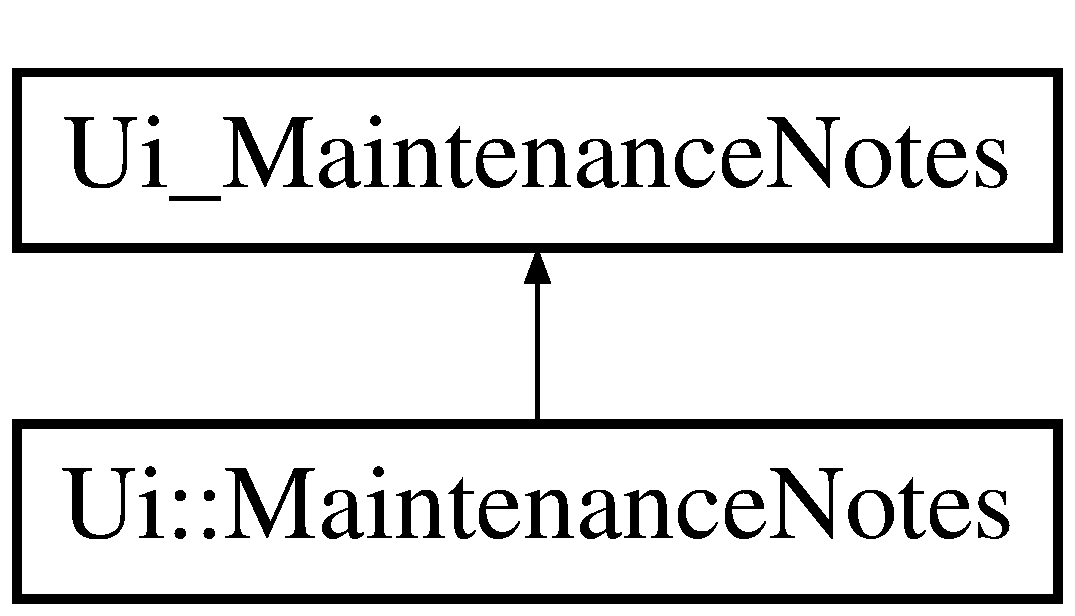
\includegraphics[height=2.000000cm]{class_ui___maintenance_notes}
\end{center}
\end{figure}
\subsection*{Public Member Functions}
\begin{DoxyCompactItemize}
\item 
\mbox{\Hypertarget{class_ui___maintenance_notes_a05be7c3c091edef3f10969a06c28b109}\label{class_ui___maintenance_notes_a05be7c3c091edef3f10969a06c28b109}} 
void {\bfseries setup\+Ui} (Q\+Dialog $\ast$\hyperlink{class_maintenance_notes}{Maintenance\+Notes})
\item 
\mbox{\Hypertarget{class_ui___maintenance_notes_ab09730e8b6fe6dda8dab7d217fb40b23}\label{class_ui___maintenance_notes_ab09730e8b6fe6dda8dab7d217fb40b23}} 
void {\bfseries retranslate\+Ui} (Q\+Dialog $\ast$\hyperlink{class_maintenance_notes}{Maintenance\+Notes})
\end{DoxyCompactItemize}
\subsection*{Public Attributes}
\begin{DoxyCompactItemize}
\item 
\mbox{\Hypertarget{class_ui___maintenance_notes_a5e89beac4a9f7461bb764220c875fe7b}\label{class_ui___maintenance_notes_a5e89beac4a9f7461bb764220c875fe7b}} 
Q\+Label $\ast$ {\bfseries Maintenance\+Notes\+Image}
\end{DoxyCompactItemize}


The documentation for this class was generated from the following file\+:\begin{DoxyCompactItemize}
\item 
ui\+\_\+maintenancenotes.\+h\end{DoxyCompactItemize}

\hypertarget{class_ui__newnew}{}\section{Ui\+\_\+newnew Class Reference}
\label{class_ui__newnew}\index{Ui\+\_\+newnew@{Ui\+\_\+newnew}}
Inheritance diagram for Ui\+\_\+newnew\+:\begin{figure}[H]
\begin{center}
\leavevmode
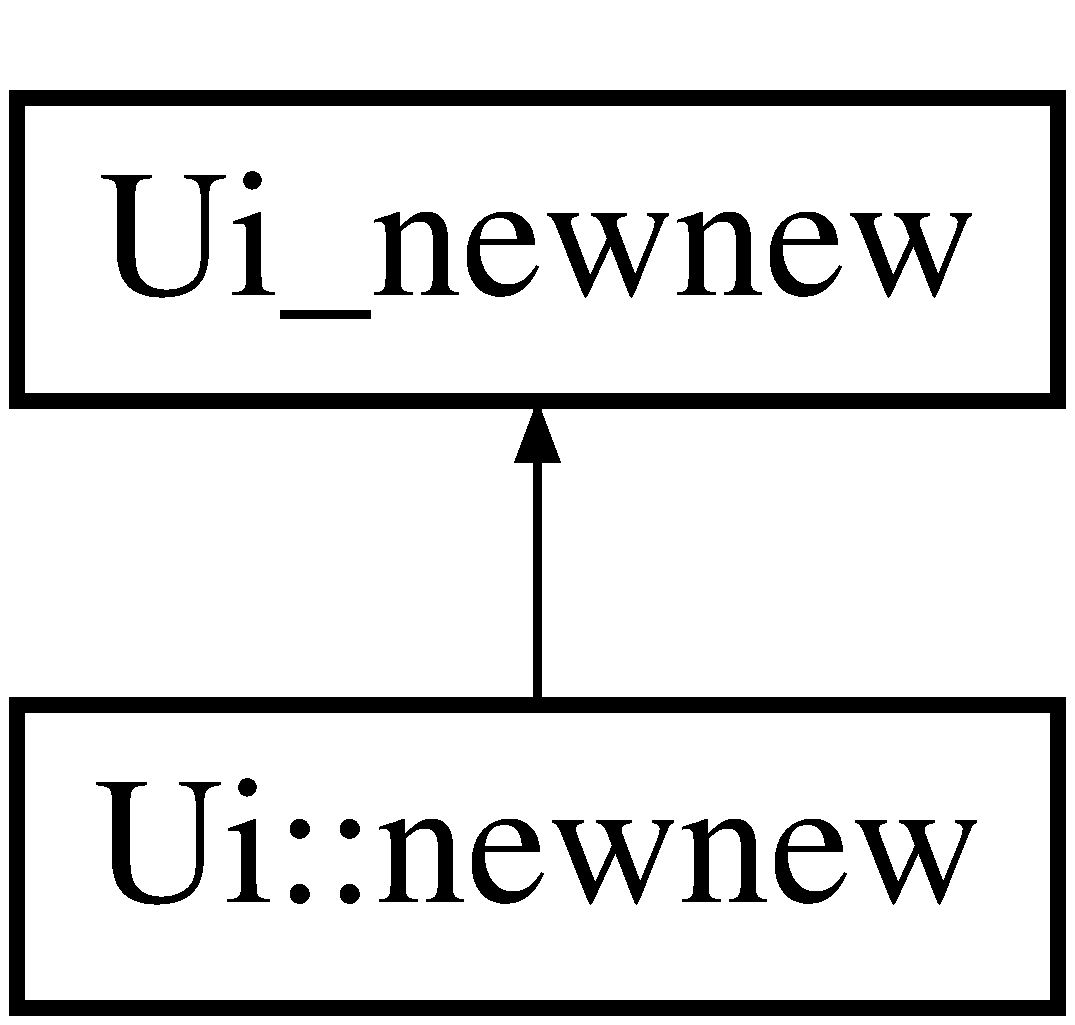
\includegraphics[height=2.000000cm]{class_ui__newnew}
\end{center}
\end{figure}
\subsection*{Public Member Functions}
\begin{DoxyCompactItemize}
\item 
\mbox{\Hypertarget{class_ui__newnew_ac0f6019b30691827488a3fd1cb21cd9b}\label{class_ui__newnew_ac0f6019b30691827488a3fd1cb21cd9b}} 
void {\bfseries setup\+Ui} (Q\+Dialog $\ast$\hyperlink{classnewnew}{newnew})
\item 
\mbox{\Hypertarget{class_ui__newnew_a7200366219e1e80993c05065825cf5c2}\label{class_ui__newnew_a7200366219e1e80993c05065825cf5c2}} 
void {\bfseries retranslate\+Ui} (Q\+Dialog $\ast$\hyperlink{classnewnew}{newnew})
\end{DoxyCompactItemize}
\subsection*{Public Attributes}
\begin{DoxyCompactItemize}
\item 
\mbox{\Hypertarget{class_ui__newnew_aac437dd2f79df915f8a3d1d3fe85738f}\label{class_ui__newnew_aac437dd2f79df915f8a3d1d3fe85738f}} 
Q\+Label $\ast$ {\bfseries label}
\item 
\mbox{\Hypertarget{class_ui__newnew_a8448fba94abfcadeb66ab4e26f25d745}\label{class_ui__newnew_a8448fba94abfcadeb66ab4e26f25d745}} 
Q\+Line\+Edit $\ast$ {\bfseries name\+Edit}
\item 
\mbox{\Hypertarget{class_ui__newnew_a941d10128eaaa55bc2cfec69d6084004}\label{class_ui__newnew_a941d10128eaaa55bc2cfec69d6084004}} 
Q\+Line\+Edit $\ast$ {\bfseries password\+Edit}
\item 
\mbox{\Hypertarget{class_ui__newnew_af579f06f624b73de7e9414c0dc865d36}\label{class_ui__newnew_af579f06f624b73de7e9414c0dc865d36}} 
Q\+Label $\ast$ {\bfseries label\+\_\+2}
\item 
\mbox{\Hypertarget{class_ui__newnew_ae01a09899032b3bdc826e49b1747551c}\label{class_ui__newnew_ae01a09899032b3bdc826e49b1747551c}} 
Q\+Label $\ast$ {\bfseries label\+\_\+3}
\item 
\mbox{\Hypertarget{class_ui__newnew_a738952f3681e7bbef5545989fac39c82}\label{class_ui__newnew_a738952f3681e7bbef5545989fac39c82}} 
Q\+Push\+Button $\ast$ {\bfseries create\+Button}
\item 
\mbox{\Hypertarget{class_ui__newnew_a575f16ae22c20108df4db3d1a47b9306}\label{class_ui__newnew_a575f16ae22c20108df4db3d1a47b9306}} 
Q\+Push\+Button $\ast$ {\bfseries login\+Button}
\item 
\mbox{\Hypertarget{class_ui__newnew_af02297af48d3cd65c21a9c257dbacca1}\label{class_ui__newnew_af02297af48d3cd65c21a9c257dbacca1}} 
Q\+Push\+Button $\ast$ {\bfseries push\+Button\+\_\+3}
\item 
\mbox{\Hypertarget{class_ui__newnew_ada3eeeb081226b3af059f4cdd4835924}\label{class_ui__newnew_ada3eeeb081226b3af059f4cdd4835924}} 
Q\+Label $\ast$ {\bfseries falling}
\item 
\mbox{\Hypertarget{class_ui__newnew_ae3af1e8c4c748cdd68e175504ea016c2}\label{class_ui__newnew_ae3af1e8c4c748cdd68e175504ea016c2}} 
Q\+Check\+Box $\ast$ {\bfseries userswitch}
\item 
\mbox{\Hypertarget{class_ui__newnew_af7424d1afed61b9406208be0ada76fa8}\label{class_ui__newnew_af7424d1afed61b9406208be0ada76fa8}} 
Q\+Combo\+Box $\ast$ {\bfseries user\+Combo}
\item 
\mbox{\Hypertarget{class_ui__newnew_a97a89aa3853e66320a6589dcc2b83dba}\label{class_ui__newnew_a97a89aa3853e66320a6589dcc2b83dba}} 
Q\+Line\+Edit $\ast$ {\bfseries admin\+Code}
\item 
\mbox{\Hypertarget{class_ui__newnew_af470042deee74a435ca20d2e492b8dbb}\label{class_ui__newnew_af470042deee74a435ca20d2e492b8dbb}} 
Q\+Label $\ast$ {\bfseries code\+Label}
\item 
\mbox{\Hypertarget{class_ui__newnew_a089c24248904c815077d88eb74be977a}\label{class_ui__newnew_a089c24248904c815077d88eb74be977a}} 
Q\+Label $\ast$ {\bfseries E\+R\+R\+O\+R\+A\+D\+M\+I\+N\+C\+O\+DE}
\end{DoxyCompactItemize}


The documentation for this class was generated from the following file\+:\begin{DoxyCompactItemize}
\item 
ui\+\_\+newnew.\+h\end{DoxyCompactItemize}

\hypertarget{class_ui___testimonials}{}\section{Ui\+\_\+\+Testimonials Class Reference}
\label{class_ui___testimonials}\index{Ui\+\_\+\+Testimonials@{Ui\+\_\+\+Testimonials}}
Inheritance diagram for Ui\+\_\+\+Testimonials\+:\begin{figure}[H]
\begin{center}
\leavevmode
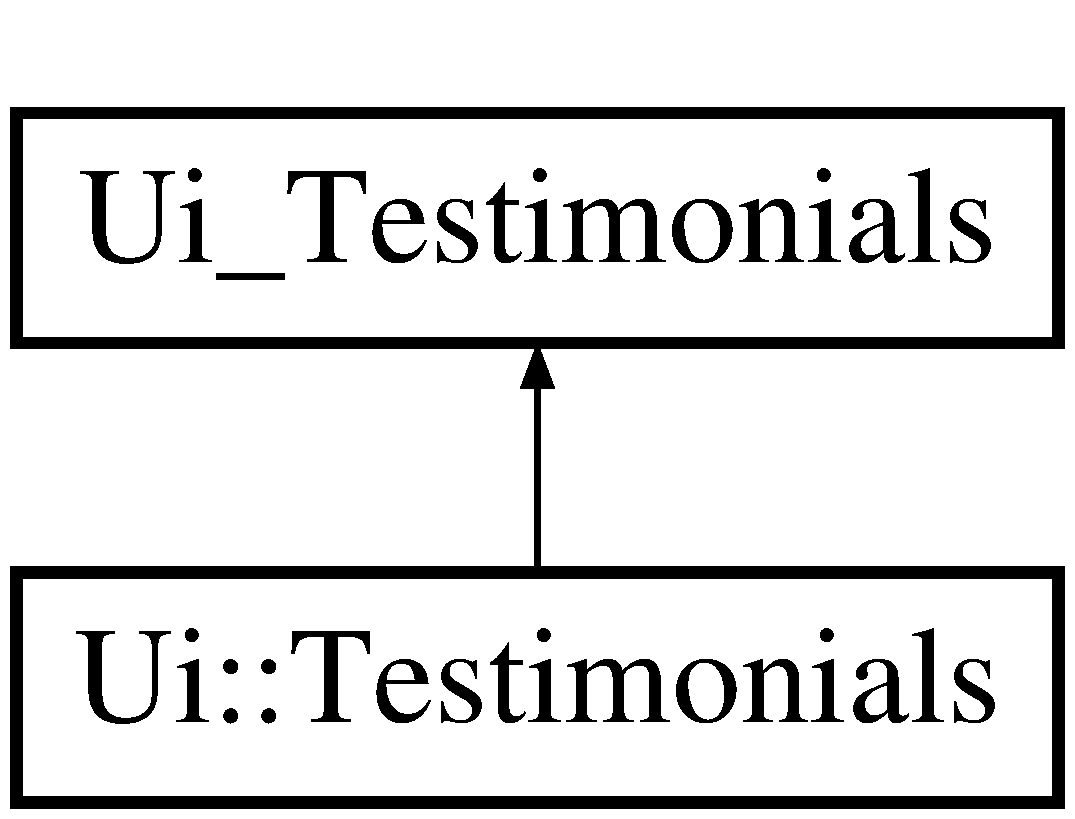
\includegraphics[height=2.000000cm]{class_ui___testimonials}
\end{center}
\end{figure}
\subsection*{Public Member Functions}
\begin{DoxyCompactItemize}
\item 
\mbox{\Hypertarget{class_ui___testimonials_a5318933ddce45cf803fce20c7931528b}\label{class_ui___testimonials_a5318933ddce45cf803fce20c7931528b}} 
void {\bfseries setup\+Ui} (Q\+Dialog $\ast$\hyperlink{class_testimonials}{Testimonials})
\item 
\mbox{\Hypertarget{class_ui___testimonials_a3d78b15bd8d7baf11793bdfcef983264}\label{class_ui___testimonials_a3d78b15bd8d7baf11793bdfcef983264}} 
void {\bfseries retranslate\+Ui} (Q\+Dialog $\ast$\hyperlink{class_testimonials}{Testimonials})
\end{DoxyCompactItemize}
\subsection*{Public Attributes}
\begin{DoxyCompactItemize}
\item 
\mbox{\Hypertarget{class_ui___testimonials_a6a8510aa73ee31fdcd18e098deea983e}\label{class_ui___testimonials_a6a8510aa73ee31fdcd18e098deea983e}} 
Q\+Text\+Browser $\ast$ {\bfseries text\+Inter\+Protocol}
\item 
\mbox{\Hypertarget{class_ui___testimonials_a0d9afd0e2c5c24e1e9bfa4fdf2700b8b}\label{class_ui___testimonials_a0d9afd0e2c5c24e1e9bfa4fdf2700b8b}} 
Q\+Text\+Browser $\ast$ {\bfseries text\+Increment\+Systems}
\item 
\mbox{\Hypertarget{class_ui___testimonials_ad3a83293eb0c1f2e53b0a3e7ddc612e0}\label{class_ui___testimonials_ad3a83293eb0c1f2e53b0a3e7ddc612e0}} 
Q\+Text\+Browser $\ast$ {\bfseries text\+Picstagram}
\item 
\mbox{\Hypertarget{class_ui___testimonials_a9ad43e8c04d09af9f37d85c278fba6c8}\label{class_ui___testimonials_a9ad43e8c04d09af9f37d85c278fba6c8}} 
Q\+Text\+Browser $\ast$ {\bfseries text\+Cloud\+Based\+Software}
\item 
\mbox{\Hypertarget{class_ui___testimonials_a09e34c99fd34c2c9ff2177295fcbead7}\label{class_ui___testimonials_a09e34c99fd34c2c9ff2177295fcbead7}} 
Q\+Text\+Browser $\ast$ {\bfseries text\+News\+Prints}
\item 
\mbox{\Hypertarget{class_ui___testimonials_a2238641b22301829a2ee62915353a226}\label{class_ui___testimonials_a2238641b22301829a2ee62915353a226}} 
Q\+Text\+Browser $\ast$ {\bfseries text\+On\+Play}
\item 
\mbox{\Hypertarget{class_ui___testimonials_ae77badabbf08c2897ac3c556fa7788ad}\label{class_ui___testimonials_ae77badabbf08c2897ac3c556fa7788ad}} 
Q\+Label $\ast$ {\bfseries On\+Play}
\item 
\mbox{\Hypertarget{class_ui___testimonials_a12ccdd81c7703cd9cc6970665895f016}\label{class_ui___testimonials_a12ccdd81c7703cd9cc6970665895f016}} 
Q\+Label $\ast$ {\bfseries Inter\+Protocol}
\item 
\mbox{\Hypertarget{class_ui___testimonials_a6f8774aa4b8e2e54e924cf40644e65ef}\label{class_ui___testimonials_a6f8774aa4b8e2e54e924cf40644e65ef}} 
Q\+Label $\ast$ {\bfseries Cloud\+Based\+Software}
\item 
\mbox{\Hypertarget{class_ui___testimonials_ae0a9f12226b6ecf914580b4e2ffbd6a2}\label{class_ui___testimonials_ae0a9f12226b6ecf914580b4e2ffbd6a2}} 
Q\+Label $\ast$ {\bfseries Picstagram}
\item 
\mbox{\Hypertarget{class_ui___testimonials_aa6ebbaa0de42607555751f586c8c8958}\label{class_ui___testimonials_aa6ebbaa0de42607555751f586c8c8958}} 
Q\+Label $\ast$ {\bfseries Increment\+Systems}
\item 
\mbox{\Hypertarget{class_ui___testimonials_a80d6ac00817cc66f1f9cc72d86e507d1}\label{class_ui___testimonials_a80d6ac00817cc66f1f9cc72d86e507d1}} 
Q\+Label $\ast$ {\bfseries News\+Prints}
\item 
\mbox{\Hypertarget{class_ui___testimonials_ae050c5064f71fc3cc8721cd2f49c93b9}\label{class_ui___testimonials_ae050c5064f71fc3cc8721cd2f49c93b9}} 
Q\+Label $\ast$ {\bfseries Guest\+Testimonial}
\item 
\mbox{\Hypertarget{class_ui___testimonials_ab91a41865930bc68a3c05c2d2eaf6c07}\label{class_ui___testimonials_ab91a41865930bc68a3c05c2d2eaf6c07}} 
Q\+Push\+Button $\ast$ {\bfseries push\+Button}
\item 
\mbox{\Hypertarget{class_ui___testimonials_acb6414bff1f9596631e267f7e59c42fb}\label{class_ui___testimonials_acb6414bff1f9596631e267f7e59c42fb}} 
Q\+Text\+Edit $\ast$ {\bfseries Testimonial\+Input}
\end{DoxyCompactItemize}


The documentation for this class was generated from the following file\+:\begin{DoxyCompactItemize}
\item 
ui\+\_\+testimonials.\+h\end{DoxyCompactItemize}

\hypertarget{class_user_list}{}\section{User\+List Class Reference}
\label{class_user_list}\index{User\+List@{User\+List}}


The \hyperlink{class_user_list}{User\+List} class -\/ holds a vector of all the users that are registered within our program; has public methods to manipulate and access all of the said users inside of the vector.  




{\ttfamily \#include $<$users.\+h$>$}

\subsection*{Public Member Functions}
\begin{DoxyCompactItemize}
\item 
\mbox{\Hypertarget{class_user_list_a29ccf809d370161ad09cb368f5f86225}\label{class_user_list_a29ccf809d370161ad09cb368f5f86225}} 
bool {\bfseries add\+User} (Q\+String name, Q\+String password, status type)
\item 
\mbox{\Hypertarget{class_user_list_a0f4aa37cd9e092f3340230d23c05351c}\label{class_user_list_a0f4aa37cd9e092f3340230d23c05351c}} 
status {\bfseries is\+User} (Q\+String name, Q\+String password)
\item 
\mbox{\Hypertarget{class_user_list_a672e71d7b506af38fac426e1a89bac12}\label{class_user_list_a672e71d7b506af38fac426e1a89bac12}} 
bool {\bfseries is\+Name\+Taken} (Q\+String name)
\item 
\mbox{\Hypertarget{class_user_list_adfeaf3c0124c4be06a3aee5ca1a13787}\label{class_user_list_adfeaf3c0124c4be06a3aee5ca1a13787}} 
Q\+String {\bfseries get\+Name} ()
\item 
\mbox{\Hypertarget{class_user_list_af9efb44315d50bd6e9cb9543864aad93}\label{class_user_list_af9efb44315d50bd6e9cb9543864aad93}} 
void {\bfseries clear} ()
\item 
\mbox{\Hypertarget{class_user_list_a8cf28059858132227f105018325d20fd}\label{class_user_list_a8cf28059858132227f105018325d20fd}} 
bool {\bfseries is\+Admin} ()
\item 
\mbox{\Hypertarget{class_user_list_ac6d715a9fe6550170cf08473e98fe31a}\label{class_user_list_ac6d715a9fe6550170cf08473e98fe31a}} 
void {\bfseries operator=} (\hyperlink{class_user_list}{User\+List} object)
\end{DoxyCompactItemize}


\subsection{Detailed Description}
The \hyperlink{class_user_list}{User\+List} class -\/ holds a vector of all the users that are registered within our program; has public methods to manipulate and access all of the said users inside of the vector. 

The documentation for this class was generated from the following files\+:\begin{DoxyCompactItemize}
\item 
users.\+h\item 
users.\+cpp\end{DoxyCompactItemize}

\hypertarget{class_vector}{}\section{Vector$<$ Type $>$ Class Template Reference}
\label{class_vector}\index{Vector$<$ Type $>$@{Vector$<$ Type $>$}}


The \hyperlink{class_vector}{Vector} class -\/ the templated vector class that is used mainly as a way to store all of the shape pointers that will be drawn on the canvas this was given to us in class; with little modification to some of the functions works very similar to the S\+TL vector.  




{\ttfamily \#include $<$Vector.\+h$>$}

\subsection*{Public Types}
\begin{DoxyCompactItemize}
\item 
\mbox{\Hypertarget{class_vector_a192547a2a73f8cfafc6bbf8bad4484bc}\label{class_vector_a192547a2a73f8cfafc6bbf8bad4484bc}} 
using {\bfseries iterator} = Type $\ast$
\item 
\mbox{\Hypertarget{class_vector_ac26885176589bc18e98f69b6917aee51}\label{class_vector_ac26885176589bc18e98f69b6917aee51}} 
using {\bfseries const\+\_\+iterator} = const Type $\ast$
\end{DoxyCompactItemize}
\subsection*{Public Member Functions}
\begin{DoxyCompactItemize}
\item 
\mbox{\Hypertarget{class_vector_a8ca8eb892b0cd3f738434dff339d5d5d}\label{class_vector_a8ca8eb892b0cd3f738434dff339d5d5d}} 
{\bfseries Vector} (int s)
\item 
\mbox{\Hypertarget{class_vector_a59fa44181957a5149face8088a516932}\label{class_vector_a59fa44181957a5149face8088a516932}} 
{\bfseries Vector} (const \hyperlink{class_vector}{Vector}$<$ Type $>$ \&src)
\item 
\mbox{\Hypertarget{class_vector_a24626edee91fdf5f8ea79c20a127c77d}\label{class_vector_a24626edee91fdf5f8ea79c20a127c77d}} 
void {\bfseries resize} (int newsize)
\item 
\mbox{\Hypertarget{class_vector_a4e0731a1b33a932943f57869acc622fd}\label{class_vector_a4e0731a1b33a932943f57869acc622fd}} 
void {\bfseries push\+\_\+back} (Type element)
\item 
\mbox{\Hypertarget{class_vector_abb56dece0fc435cfeb4da8a469606e59}\label{class_vector_abb56dece0fc435cfeb4da8a469606e59}} 
void {\bfseries reserve} (int newalloc)
\item 
\mbox{\Hypertarget{class_vector_aa2cd243dd27f6e21b4d240929fb96878}\label{class_vector_aa2cd243dd27f6e21b4d240929fb96878}} 
int {\bfseries size} () const
\item 
\mbox{\Hypertarget{class_vector_ae0c31c5131b18b6e5a1e24c31fc38fca}\label{class_vector_ae0c31c5131b18b6e5a1e24c31fc38fca}} 
int {\bfseries capacity} () const
\item 
\mbox{\Hypertarget{class_vector_a7e9dcb119d679a109ef0fe34d884451c}\label{class_vector_a7e9dcb119d679a109ef0fe34d884451c}} 
\hyperlink{class_vector}{Vector}$<$ Type $>$ \& {\bfseries operator=} (const \hyperlink{class_vector}{Vector}$<$ Type $>$ \&src)
\item 
\mbox{\Hypertarget{class_vector_a1858c8faef5af17ad87eacede83ef0d8}\label{class_vector_a1858c8faef5af17ad87eacede83ef0d8}} 
Type \& {\bfseries operator\mbox{[}$\,$\mbox{]}} (int n)
\item 
\mbox{\Hypertarget{class_vector_afcf679a0343376f9cc44e31b9d51338c}\label{class_vector_afcf679a0343376f9cc44e31b9d51338c}} 
const Type \& {\bfseries operator\mbox{[}$\,$\mbox{]}} (int n) const
\item 
\mbox{\Hypertarget{class_vector_a679da56b02db310bbe560567749a38af}\label{class_vector_a679da56b02db310bbe560567749a38af}} 
iterator {\bfseries begin} ()
\item 
\mbox{\Hypertarget{class_vector_a81f211393ac5acf7ea0a021d81456b60}\label{class_vector_a81f211393ac5acf7ea0a021d81456b60}} 
const\+\_\+iterator {\bfseries begin} () const
\item 
\mbox{\Hypertarget{class_vector_ab4384e8d78cc67530edcff225becb88b}\label{class_vector_ab4384e8d78cc67530edcff225becb88b}} 
iterator {\bfseries end} ()
\item 
\mbox{\Hypertarget{class_vector_a90af5eec59b6d5252dfb6139c43dcead}\label{class_vector_a90af5eec59b6d5252dfb6139c43dcead}} 
const\+\_\+iterator {\bfseries end} () const
\item 
\mbox{\Hypertarget{class_vector_aec5c8c190b418825e31204d26a13b923}\label{class_vector_aec5c8c190b418825e31204d26a13b923}} 
iterator {\bfseries insert} (iterator p, const Type \&val)
\item 
\mbox{\Hypertarget{class_vector_a77c26be8457ea5786f01da40e59c0404}\label{class_vector_a77c26be8457ea5786f01da40e59c0404}} 
iterator {\bfseries erase} (iterator p)
\end{DoxyCompactItemize}


\subsection{Detailed Description}
\subsubsection*{template$<$class Type$>$\newline
class Vector$<$ Type $>$}

The \hyperlink{class_vector}{Vector} class -\/ the templated vector class that is used mainly as a way to store all of the shape pointers that will be drawn on the canvas this was given to us in class; with little modification to some of the functions works very similar to the S\+TL vector. 

The documentation for this class was generated from the following file\+:\begin{DoxyCompactItemize}
\item 
Vector.\+h\end{DoxyCompactItemize}

%--- End generated contents ---

% Index
\backmatter
\newpage
\phantomsection
\clearemptydoublepage
\addcontentsline{toc}{chapter}{Index}
\printindex

\end{document}
